\pdfminorversion=4
\pdfobjcompresslevel=0

\newif\ifpaperonly
\paperonlyfalse
%% \paperonlytrue

\newif\iftestonly
\testonlyfalse
\testonlytrue

\documentclass[
draft,
fontsize=11pt,
a4paper,
twoside,
german,
headsepline=true,
footsepline=false,
automark,
headings=normal,
appendixprefix,
open=any,
cleardoublepage=plain,
abstract=true,
index=totoc,
listof=totoc,
bibliography=totoc,
BCOR9mm,
]{scrreprt}

\usepackage{ifdraft}

\usepackage[ngerman]{babel}
\usepackage[utf8]{inputenc}
\usepackage[]{geometry} % Seitenraender
\usepackage[final]{graphicx}
\usepackage{acronym}
\usepackage{bibgerm}
\usepackage{calc}
\usepackage[table]{xcolor}
\usepackage{scrpage2}
\usepackage{tabularx}
\usepackage{threeparttable}
\usepackage{booktabs}
\usepackage{ngerman}
\usepackage{capt-of}
\usepackage{longtable}
\usepackage{amsmath}
\usepackage{pdfpages}
\usepackage{todonotes}
\usepackage{listings}
\usepackage[rightcaption]{sidecap}

\setkomafont{disposition}{\normalcolor\bfseries}
\lstloadlanguages{[LaTeX]TeX}

%% \usepackage[plainpages=false,pdfpagelabels]{hyperref}
\ifpaperonly
  \usepackage[plainpages=false, pdfpagelabels, hidelinks, colorlinks=false, pdfpagelayout=TwoPageRight]{hyperref}
\else
  \definecolor{url}{rgb}{0.7 0 0.2}
  \definecolor{link}{rgb}{0.0 0.0 0.8}
  \definecolor{cite}{rgb}{0.0 0.5 0}
  \usepackage[plainpages=false, pdfpagelabels, hidelinks, colorlinks=true, linkcolor=link, citecolor=cite, urlcolor=url, pdfpagelayout=TwoPageRight]{hyperref}
\fi

\usepackage{amssymb}
\usepackage[font=normal]{subcaption}
\usepackage{scrhack}

\usepackage{graphicx}
\usepackage{transparent}

% Times New
\usepackage{newtxtext}
\usepackage{newtxmath}
\usepackage{pifont}

% Overflows und Fehlkerning reduzieren
\usepackage[
        activate={true,nocompatibility},
        final,
        tracking=true,
        kerning=true,
%%        spacing=true,
        factor=1100,
        stretch=10,
        shrink=10
]{microtype}
\usepackage[range-phrase={\,bis\,},binary-units,retain-explicit-plus]{siunitx}

\usepackage[version=3]{mhchem}
\usepackage{cite}
\usepackage{verbatim}
\usepackage[percent]{overpic}


\graphicspath{{img/},{img-results/}}

\pagestyle{scrheadings} % Standart Kopf- und Fußzeile
\setkomafont{pageheadfoot}{\small\scshape} % for new Koma Script

% ---------------------------------------------------------------------
%\setcounter{secnumdepth}{2}
%\setcounter{chapter}{-1}
\setcounter{tocdepth}{2}

% ---------------------------------------------------------------------
%\sloppy % weniger Worttrennungen, größere Wortabstände
\fussy % viele Worttrennungen, "schönere" Wortabstände

% ---------------------------------------------------------------------
%\flushbottom % Ausrichtung der Seitenenden jeweils auf
% gleicher Höhe

% ---------------------------------------------------------------------
%\sloppypar % Das hier relaxt die Einstellungen zum Wortabstand
% extrem. Damit ragen keine Worte über den rechten
% Zeilenabstand hinaus. Dafür muß stärker auf
% Wortabstand geachtet werden, der kann dann ziemlich
% groß werden. Man erhält aber keine Meldung mehr
% über underfull boxes.

%Hiermit kann man das gleiche mit weniger Holzhammer erreichen:
%\setlength{\tolerance}{2000} % Strafpunkt für Zeilenumbruch
%\setlength{\emergencystretch}{3pt} % Soweit dürfen einzelne Worte mehr
% auseinandergezogen werden
%\setlength{\hfuzz}{1pt} % Macht den rechten Rand um bis zu 1pt
% flatterig.

% ---------------------------------------------------------------------
%Vermeiden einzelner Zeilen am Ende einer Seite oder oben auf einer neuen Seite
\clubpenalty10000
\widowpenalty10000

% eigene Definitionen
\newcommand{\BigO}[1]{$\mathcal{O}(#1)$}
\newcommand{\mergedcell}[2][l]{\begin{tabular}[#1]{@{}l@{}}#2\end{tabular}}
\newcommand{\cmark}{\ding{51}}
\newcommand{\ccross}{\ding{55}}

\definecolor{Green}{rgb}{0.0 1.0 0.0}
\definecolor{Yellow}{rgb}{1.0 1.0 0.0}
\definecolor{Red}{rgb}{1.0 0.0 0.0}
\definecolor{lightgray}{gray}{0.9}

\newcolumntype{C}{>{\centering\arraybackslash}X}
\newcolumntype{R}{>{\hsize=0.15\textwidth}X}

\newcommand{\cG}[1]{\transparent{5.0}\cellcolor{Green}#1}
\newcommand{\cY}[1]{\transparent{5.0}\cellcolor{Yellow}#1}
\newcommand{\cR}[1]{\transparent{5.0}\cellcolor{Red}#1}

\DeclareSIUnit\gpcc{\gram\per\cubic\centi\meter}
\def\oddrowcolors{\rowcolors{1}{}{black}}
\def\evenrowcolors{\rowcolors{1}{black}{}}

%% rowcolors fix: This makes the rowcolors boxes transparent, so they won't overwrite hline and vline commands (i.e. table borders)
\makeatletter
\def\CT@@do@color{%
  \global\let\CT@do@color\relax
        \@tempdima\wd\z@
        \advance\@tempdima\@tempdimb
        \advance\@tempdima\@tempdimc
        \kern-\@tempdimb
\transparent{0.2}%
        \leaders\vrule
                \hskip\@tempdima\@plus 1fill
        \kern-\@tempdimc
        \hskip-\wd\z@ \@plus -1fill }
\makeatother
\setlength{\arrayrulewidth}{0.6pt}

%threeparttable textwidth
\renewcommand{\TPTminimum}{\textwidth}

%% avoid the [inline] option of todo
\newcommand{\todoline}[1]{\todo[inline]{#1}{}}
\newcommand{\continuehere}{\todoline{continuehere}{}}

\newcommand{\ignore}[1]{}

%% disable todo
\ifdraft{
  \newcommand{\Si}[2]{\todo{Tippfehler: \\Si statt \\SI}\SI{#1}{#2}}
}{
  \renewcommand{\todoline}[1]{}
  \renewcommand{\todo}[1]{}
}

\newcommand{\qqquad}[0]{\qquad\quad}
\newcommand{\pot}[1]{\texttt{#1}}

\newcommand{\chemlegend}[1]{\begin{minipage}[c]{0.7cm}\includegraphics[width=\textwidth]{#1}\end{minipage}}
\newcommand{\chemlegendce}[1]{\chemlegend{#1}\ce{#1}}

% asd 
%% \renewcommand{\oddrowcolors}{}
%% \renewcommand{\evenrowcolors}{}

%======================================================================
%	Metadaten
%======================================================================
%	$Id$
%	Original template: Matthias Kupfer
%======================================================================

\newcommand{\dcsubject}{Masterarbeit}
\newcommand{\dctitle}{Atomistische Modellierung und Simulation des Filmwachstums bei Gasphasenabscheidungen}
%% \newcommand{\dctitle}{Modellierung und Simulation von Schichtabscheidungen aus der Gasphase}
\newcommand{\dcsubtitle}{} % Untertitel, falls erforderlich

\newcommand{\dcauthortitle}{B.Sc.}
\newcommand{\dcauthorlastname}{Lorenz}
\newcommand{\dcauthorfirstname}{Erik E.}
\newcommand{\dcauthoremail}{erik.e.lorenz@gmail.com} 
\newcommand{\dcdate}{\today}

\newcommand{\dcplace}{Chemnitz} % Ort, kann an der TU meist so bleiben
\newcommand{\dcuni}{Technische Universität \dcplace}
\newcommand{\dcdepart}{Fakultät für Naturwissenschaften} % Fakultätsangabe
\newcommand{\dcinstitute}{Institut für Physik}

\newcommand{\dcinstituteext}{Fraunhofer-Institut für Elektronische Nanosysteme}
\newcommand{\dcdepartext}{Abteilung Back-End of Line} % Fakultätsangabe

\newcommand{\dcexaminerfirst}{Prof. Dr. Stefan E. Schulz}
\newcommand{\dcdepartfirst}{Fakultät für Elektrotechnik und Informationstechnik} % Fakultätsangabe
\newcommand{\dcproffirst}{Technologien der Nanoelektronik} % Angabe der Professur

\newcommand{\dcexaminersecond}{N.N.}
\newcommand{\dcdepartsecond}{\dcdepart} % Fakultätsangabe
\newcommand{\dcprofsecond}{N.N.} % Angabe der Professur
\newcommand{\dcinstitutesecond}{\dcinstitute}

\newcommand{\dcadvisor}{Dr. Jörg Schuster}
\newcommand{\dcinstituteadvisor}{\dcinstituteext}
\newcommand{\dcdepartadvisor}{\dcdepartext}
\newcommand{\dcgroupadvisor}{Simulationsgruppe}

\newcommand{\dckeywords}{Enter Keywords Here}

%%======================================================================
% Einstellungen des Hyperref-Paketes
\hypersetup{%    
	pdftitle	= {\dctitle}, %
	pdfsubject	= {\dcsubject, \dcdate}, %
	pdfauthor	= {\dcauthorfirstname~\dcauthorlastname, \dcauthoremail}, %
	pdfkeywords	= {\dckeywords}, %
	pdfcreator	= {pdfTeX with Hyperref and Thumbpdf}, %
	pdfproducer	= {LaTeX, hyperref, thumbpdf}, %
	% weitere PDF-Einstellungen in hyperref.cfg
}
%%======================================================================


\begin{document}

\iftestonly
  \section{Laufzeitmaße für das Parsivald}

Wie für Laufzeitanalysen üblich, werden die Laufzeiten mit $T$ bezeichnet und sollten nicht mit den ähnlich bezeichneten Temperaturwerten verwechselt werden.
\todoline{Hinweis auf ISO80000-1:2009 oder die äquivalente DIN?}

\subsection{Ereignis-Laufzeit $T_\text{E}$}

Die Auswahl und Verarbeitung eines Ereignisses in KMC-Algorithmen ist mit einer Laufzeit~$T_\text{E}$ verbunden, die sich aus der Laufzeit von Suchoperationen $T_\text{KMC}$, der Laufzeit von Serialisierungen und Deserialisierungen zur Datenübertragung zwischen Host und Worker $T_\text{Ser.}$ und $T_\text{Des.}$ sowie der Laufzeit für die Konnektivitätsprüfung $T_\text{Konn.}$ zusammen setzt:

\begin{equation}
T_\text{E} = T_\text{KMC} + T_\text{Ser.} + T_\text{Des.} + T_\text{Konn.}
\end{equation}
\todo{bessere Variable als $n$ für die Zahl der lokalen Atome finden}Die Laufzeiten zur Serialisierung $T_\text{Ser.}$ und zur Deserialisierung $T_\text{Des.}$ der Atompositionen sind mit \BigO{n} dabei gegenüber der Konnektivitätsprüfung (\BigO{n^2}) verschwindend gering.
$T_\text{KMC}$ hängt von der genutzten Datenstruktur ab und ist unter Verwendung eines Octrees mit Access Caching in der aktuellen Implementierung mit einer Laufzeit von \BigO{n} verbunden.
\todo{Aus den in Kapitel~\ref{results} vorgestellten Simulationen gehen Laufzeiten von $T_\text{E} \approx \SI{30}{\milli\second}$ hervor. ?}

\subsection{Ereignis-Durchsatz $R_\text{E}$}

Als Ereignis-Durchsatz wird nachfolgend die Zahl der vom Host zur MD-Berechnung bereit gestellten Ereignisse pro Zeiteinheit bezeichnet.
Damit handelt es sich eigentlich um eine Rate von Ereignissen, die jedoch nicht mit der Ereignisrate aus dem KMC-Formalismus verwechselt werden sollte.
Der Wert des Ereignis-Durchsatzes beschreibt in diesem Kontext die maximal mögliche Zahl von ausgewählten Ereignissen pro Zeiteinheit und ist unabhängig von den Eigenschaften der MD-Berechnungen.
In der aktuellen Implementierung führt ein serieller Host-Prozess alle Vor- und Nachbereitungen von Ereignissen durch, weshalb sich der Ereignis-Durchsatz als reziproker Wert der Ereignis-Laufzeit $T_\text{E}$ ergibt:

\begin{equation}
  R_\text{E} = \frac{1}{T_\text{E}}
\end{equation}

\subsection{MD-Laufzeit $T_\text{MD}$}

Die Zeit von der Übertragung eines Ereignisses an einen Worker bis zur Vollendung der molekulardynamischen Simulationen wird im Folgenden als MD-Laufzeit $T_\text{MD}$ bezeichnet.
Sie ist hauptsächlich von den benutzten Kraftfeldern abhängig, wird jedoch auch durch die durchgeführten MD-Operationen, die Relaxationszeit, sowie die Größe der MD-Box und die damit verbundene Zahl der Atome beeinflusst.
Vom KMC-Algorithmus ist sie hingegen unabhängig, wodurch sie sich als elementarer Wert der Laufzeiteigenschaften von Parsivald-Simulationen ergibt.

\subsection{Worker-Laufzeit $T_\text{worker}$}

Ähnlich zur Ereignis-Laufzeit ergibt sich die Worker-Laufzeit, wobei die Serialisierungs- und Deserialisierungs-Operationen gegenüber den MD-Berechnungen verschwindend sind, weshalb nachfolgend die MD-Laufzeit an Stelle der Worker-Laufzeit genutzt werden soll.
\begin{align}
  T_\text{worker} & = T_\text{Ser.} + T_\text{Des.} + T_\text{MD} \\
                  & \approx T_\text{MD}
\end{align}

\subsection{Serielle Laufzeit $T_1$}

Die serielle Laufzeit $T_1$ bezeichnet die Laufzeit eines Programmes unter Nutzung eines einzigen Prozesses.
Damit ist sie von der Laufzeit zur Vorbereitung der Simulation $T_\text{start}$, der Laufzeit zum Abschluss der Simulation $T_\text{end}$ und den eben vorgestellten Ereignis- und MD-Laufzeiten $T_\text{E}$ und $T_\text{MD}$ sowie der Zahl der Ereignisse $N_\text{E}$ abhängig.
Die Laufzeiten zur Vorbereitung und zum Abschluss der Simulation sind dabei verschwindend gering.

\begin{align}
  T_1 & = T_\text{start} + N_\text{E} \cdot (T_\text{E} + T_\text{MD}) + T_\text{end} \\
      & \approx N_\text{E} T_\text{E} + N_\text{E} T_\text{MD}
\end{align}

\subsection{Anzahl der parallelen Prozesse $p$}

Ein wichtiges Maß für die Effizienz eines parallelen Prozess ist die Zahl der aktiven parallelen Prozesse $p$.
Aufgrund der variablen Zahl der gleichzeitig aktiven Prozesse in Parsivald-Simulationen wird nachfolgend mit $p$ die mittlere Zahl der aktiven MD-Prozesse bezeichnet.
Für die Zahl der Parallelen Prozesse ergeben sich zwei obere Schranken in der maximalen Bedeckung der Oberfläche mit MD-Boxen einerseits und dem Ereignis-Durchsatz andererseits.
Diese Schranken werden erreicht, wenn der Parsivald-Simulation eine praktisch unbegrenzte Zahl an Worker-Prozessen zur Verfügung steht, von denen aber nur $p_\text{max}$ Prozesse parallel genutzt werden können.

Für kleine Simulationsräume lässt sich die maximale Anzahl von Ereignissen $p_\text{max,1}$ aus der dichtesten Packung von MD-Boxen der Breite $w_\text{MD}$, Tiefe $d_\text{MD}$ und Fläche $A_\text{MD} = w_\text{MD} \cdot d_\text{MD}$ auf der Oberfläche (gleichartige Symbole) abschätzen:
\begin{align}
  p_\text{max,1} & = \left\lfloor\frac{w_\text{sim}}{w_\text{MD}}\right\rfloor \cdot \left\lfloor\frac{d_\text{sim}}{d_\text{MD}}\right\rfloor \\
  & \approx \left\lfloor\frac{A_\text{sim}}{A_\text{MD}}\right\rfloor
\end{align}
\todoline{Abbildung aus Vortrag}
Bei großen Simulationsräumen ergibt sich die Grenze im Ereignis-Durchsatz des Hauptprozesses in Verbindung mit der Laufzeit von MD-Simulationen:
\begin{align}
  p_\text{max,2} & = R_\text{E} \cdot T_\text{MD} \\
                 & = \frac{T_\text{MD}}{T_\text{E}}
\end{align}

Somit lässt sich die obere Schranke der Anzahl paralleler Prozesse als Minimum der beiden Werte abschätzen.
\begin{align}
  p_\text{max} & = \min(p_\text{max,1}, p_\text{max,2}) \\
  & = \min\left(\left\lfloor\frac{A_\text{sim}}{A_\text{MD}}\right\rfloor, \frac{T_\text{MD}}{T_\text{E}}\right)
\end{align}

\subsection{Workerdichte $\rho_\text{worker}$}

Ein Parsivald-spezifisches Leistungsmaß ergibt sich mit der Workerdichte, welche das Verhältnis der mittleren Anzahl der parallelen Prozesse $p$ zur maximalen Zahl gleichzeitiger Ereignisse für kleine Räume $p_\text{max,1}$ beschreibt und somit auch für verschiedene Kraftfelder und Substratgrößen vergleichbar ist.
\begin{equation}
  \rho_\text{worker} = \frac{p}{p_\text{max,1}}
\end{equation}
Aufgrund der stochastischen Verteilung der Ereignisorte in Parsivald-Simulationen werden im Schnitt nur ca. \todo{woher kommt der Wert?}\SI{40}{\percent} Workerdichte erreicht.

\subsection{Parallele Laufzeit $T_p$}

Die parallele Laufzeit $T_p$ bezeichnet die Laufzeit eines Programmes unter Nutzung mehrerer paralleler Prozesse.
Sämtliche KMC-Operationen werden in Parsivald vom Hauptprozess verarbeitet, während die MD-Simulationen von unabhängigen MD-Prozessen durchgeführt werden:

\begin{align}
  T_p & = T_\text{start} + N_\text{E} \cdot (T_\text{E} + \frac{T_\text{MD}}{p}) + T_\text{end} \\
      & \approx N_\text{E} T_\text{E} + \frac{N_\text{E} T_\text{MD}}{p}
\end{align}

\subsection{Speedup $S_p$}

Beim Speedup handelt es sich um das Verhältnis der linearen Laufzeit zur parallelen Laufzeit.
Damit ist er ein in der Laufzeitanalyse übliches Maß für die Effizienz paralleler Prozesse.
\begin{align}
  S_p & = \frac{T_1}{T_p}                                                     \\
      & = \frac{T_\text{E} + T_\text{MD}}{T_\text{E} + \frac{T_\text{MD}}{p}} \\
      & = 1 + \frac{T_\text{MD} (p - 1)}{p T_\text{E} + T_\text{MD}}
\end{align}
Für serielle Parsivald-Läufe ($p=1$) liegen praktisch keine Leistungseinbußen ($S_1=1$) vor, während der Speedup $S_\text{max}$ für große Simulationen, welche eine große Zahl von paralleler MD-Rechnungen $p_\text{max,2}$ zulassen, durch den Ereignis-Durchsatz und die MD-Laufzeiten determiniert wird.
Dabei ist nicht $S_\text{max}$ selbst maximal, sondern die Zahl der parallelen Prozesse.
\begin{align}
  S_\text{max} & = 1 + \frac{T_\text{MD}^2 R_\text{E} - T_\text{MD}}{T_\text{MD} R_\text{E} T_\text{E} + T_\text{MD}} \\
  & = \frac{1}{2} + \frac{1}{2}\frac{T_\text{MD}}{T_\text{E}} \\
  & > 1 \qquad(T_\text{MD} > T_\text{E})
\end{align}

\todoline{Kann ich aus den Formeln einen Speedup-Plot erstellen? Denke, schon.}

\subsection{Parallele Effizienz $E_p$}

Die parallele Effizienz $E_p$ ist als Verhältnis aus dem Speedup $S_p$ zur Zahl der Prozesse $p$ definiert.
Somit ergibt sich 
\begin{align}
  E_p & = \frac{S_p}{p} \\
  & = \frac{1}{p} + \frac{p T_\text{MD} - T_\text{MD}}{p^2 T_\text{E} + p T_\text{MD}} \\
  E_\text{max} & = \frac{1}{2} + \frac{T_\text{E}}{2 T_\text{MD}}
\end{align}
Bei einer unbegrenzten Anzahl an Worker-Prozessen steigt somit der Speedup mit der MD-Laufzeit, während die parallele Effizienz sinkt.
Einerseits lassen sich mit längerer MD-Laufzeit mehr parallele Worker mit Ereignissen versorgen, andererseits sinkt die parallele Effizienz mit der Zahl der Prozesse.
Weder der Speedup noch die parallele Effizienz treffen dabei eine Aussage über die eigentliche Laufzeit $T_p$ der Simulation, welche für $p = p_\text{max,1}$ linear mit der MD-Laufzeit $T_\text{MD}$ steigt.
Somit ist die Laufzeit von Parsivald-Simulationen theoretisch unabhängig von der Größe des Substrates, solang eine ausreichende Zahl von Worker-Prozessen zur Verfügung steht, der Ereignis-Durchsatz des Host-Prozesses aber noch nicht erreicht wurde.

\subsection{Abschätzung des parallelen Anteils $P$ (Parallelisierbarkeit)}

Aus den oben gegebenen Formeln lässt sich der serielle Anteil $S$ der Laufzeit anhand der maximalen Zahl der Worker $p = p_\text{max,1}$ abschätzen:
\begin{align}
  S & = \frac{T_\text{E}}{T_\text{MD} + T_\text{E}} \\
    & = \frac{1}{p + 1}
\end{align}
Aus der Beziehung $S + P = 1$ ergibt sich eine Parallelisierbarkeit $P$ von Parsivald aus der Zahl der Worker $p$ wie folgt:
\begin{equation}
  P = \frac{p}{p+1}
\end{equation}

\else
  %======================================================================
%	Titelseite 
%======================================================================

% Wir setzten hier die Seitennummerierung auf Großrömisch, auch wenn diese
% nicht auf dem "Papier" erscheint. Es dient nur der internen Zählung der
% Seiten im hyperref-Paket, welches für die Seitennummerierung in den PDFs
% zuständig ist. Ohne diesen Trick kommen ein paar sinnlose Warnungen und
% die Seiten-Navigation im Adobe Reader kann durcheinander geraten.
\pagenumbering{Roman}


%%======================================================================
%% Schmutztitel
%%======================================================================
%\extratitle{
%	\usekomafont{disposition}\mdseries 
%	\begin{center}
%		\Huge \dcsubject\\[1.5ex]
%		\hrule
%		\vspace*{\fill}
%		\includegraphics{TUC_deutsch_einzeile_CMYK}
%	\end{center}
%}

%%======================================================================
%% Titelkopf
%%======================================================================
\titlehead{
	\vspace*{-1.5cm}
	\begin{center}
		\raisebox{-1ex}{\includegraphics[scale=1.1]{img/logo_tu_tailored}}\\
		\hrulefill \\[1em]
		{\Large\dcdepartsecond}\\[0.2em] 
		\dcinstitutesecond\\[0.5em]
%		{\Large\dcdepartsecond}\\[0.5em] 
%		\dcprofsecond
	\end{center}
	\vspace*{0.1cm}
	\begin{center}
		\raisebox{-1ex}{\includegraphics[scale=1.2]{img/logo_fhg_tailored}}\\
		\hrulefill \\[1em]
		{\Large\dcdepartthird}\\[0.2em] 
		\dcprofthird\\[0.5em]
	\end{center}
	\vspace*{0.5cm}
}



%%======================================================================
%% Subjekt
%%======================================================================
\subject{\huge\textnormal{\textsc{\dcsubject}}}


%%======================================================================
%% Titel
%%======================================================================
\title{\huge
	\dctitle
	\\
	\dcsubtitle
	\vspace*{-0.4em}
}

%%======================================================================
%% Autor des Dokumentes
%%======================================================================
\author{\dcauthortitle~\dcauthorfirstname~\dcauthorlastname}
	
%%======================================================================
%% Ort, Datum
%%======================================================================
\date{\dcplace, den \dcdate
}


%%======================================================================
%% Publishers
%%======================================================================
\publishers{
		\begin{tabbing}
			\hspace*{10.1em}\=\kill
			\hspace*{4.8em}{Gutachter:}\>\dcexaminerfirst\\[-0.2em]
								  \>{\small\dcproffirst}\\[0.2em]
								  \>\dcexaminersecond\\[-0.2em]
								  \>{\small\dcprofsecond}\\
		\end{tabbing}	
	\vspace*{-7em}
}

%%======================================================================
%% bibliografische Angaben
%%======================================================================
\lowertitleback{
\textbf{\dcauthorlastname, \dcauthorfirstname}\\
\textit{\dctitle}\\
%\dcsubject,~\dcdepart\\
\dcsubject\\
\dcuni,~\ifcase\month\or
  Januar\or Februar\or März\or April\or Mai\or Juni\or
    Juli\or August\or September\or Oktober\or November\or Dezember\fi
    ~\number\year\\
Stichworte: \dckeywords
}

%%======================================================================
%% maketitle
%%======================================================================

\maketitle

%%======================================================================
%% Danksagung
%%======================================================================
%\thispagestyle{empty}
%\null\vfil
%\begin{center}
%\usekomafont{disposition}\textbf{Danksagung}
%\vspace{-.5em}\vspace{\parsep}
%%
%% Hier steht der Text für die Danksagung
%%
%\end{center}
%\par\vfil\null
%\cleardoubleemptypage
  
%%======================================================================
%%      Kurzfassung / Abstract
%%======================================================================
%\def\abstractname{Abstract} 	% Wenn der Text "Zusammenfassung" erscheinen 
								% soll, dann muß dies auskommentiert werden
				
\pagenumbering{roman}
\begin{abstract}

\end{abstract}

%%======================================================================
%%      Inhaltsverzeichnis
%%======================================================================
%\clearpage

%\cleardoubleemptypage

%\pdfbookmark{Inhaltsverzeichnis}{Inhaltsverzeichnis}
\tableofcontents
%\setcounter{tocdepth}{2}

%%======================================================================
%%      Abbildungsverzeichnis
%%======================================================================
%\cleardoublepage
\markboth{Abbildungsverzeichnis}{Abbildungsverzeichnis}
\listoffigures

%%======================================================================
%%      Tabellenverzeichnis
%%======================================================================
%\cleardoublepage
\markboth{Tabellenverzeichnis}{Tabellenverzeichnis}
\listoftables

%======================================================================
%  Literaturverzeichnis
%======================================================================
%\cleardoublepage
%\manualmark
%\markboth{Literaturverzeichnis}{Literaturverzeichnis}
%\bibliographystyle{unsrt}
%\bibliographystyle{own}
%\bibliography{literatur}

%%======================================================================
%%      Algorithmenverzeichnis
%%======================================================================
%\renewcommand{\listalgorithmname}{Algorithmenverzeichnis}
%\cleardoublepage
%\addcontentsline{toc}{chapter}{Algorithmenverzeichnis}
%\listofalgorithms

%%======================================================================
%%      Abkuerzungsverzeichnis
%%======================================================================
%\cleardoublepage
\chapter*{Abkürzungsverzeichnis}
\addcontentsline{toc}{chapter}{Abkürzungsverzeichnis}
\markboth{Abkürzungsverzeichnis}{Abkürzungsverzeichnis}
\def\listacronymname{Abkürzungsverzeichnis}

\newcolumntype{Y}{>{\flushleft\arraybackslash}X}

%\begin{acronym}[SQL]
% \acro{CNTs}{Kohlenstoffnanoröhrchen (engl. Carbon Nanotubes, CNTs)}
% \acro{DFT}{Dichtefunktionaltheorie}
%\end{acronym}

\def\arraystretch{1.5}
\begin{tabularx}{\linewidth}{lll}
ALD	&	Atomic Layer Deposition	&	Atomlagenabscheidung	\\
CVD	&	Chemical Vapor Deposition	&	Chemische Gasphasenabscheidung	\\
PVD	&	Physical Vapor Deposition	&	Physikalische Gasphasenabscheidung	\\
RDF	&	Radial Distribution Function	&	Radiale Verteilungsfunktion	\\
Parsivald	&	\multicolumn{2}{X}{Parallel Atomistic Reaction Simulator for Vapor and Atomic Layer Depositions}	\\
\end{tabularx}

%\begin{longtable}{lll}
%
%MOSFET & Metall-Oxid-Halbleiter-Feldeffekttransistor & metal-oxid-semiconductor field-effect transistor \\
%
%\end{longtable}


\chapter*{Symbolverzeichnis}
\addcontentsline{toc}{chapter}{Symbolverzeichnis}
\markboth{Abkürzungsverzeichnis}{Symbolverzeichnis}
\def\listacronymname{Symbolverzeichnis}

\begin{tabularx}{\linewidth}{ll}
\end{tabularx}

%\printglosstex(acr)

%%======================================================================
%%      Ende
%%======================================================================
\cleardoublepage
\pagenumbering{arabic} % Fäng erneut bei 1 an.

  \pagenumbering{roman}
  \begin{abstract}
Gasphasenabscheidungen werden zur Produktion dünner Schichten in der Mikro- und Nanoelektronik benutzt, um eine präzise Kontrolle der Schichtdicke im Sub-Nanometer-Bereich zu erreichen.
Elektronische Eigenschaften der Schichten werden dabei von strukturellen Eigenschaften determiniert, deren Bestimmung mit hohem experimentellem Aufwand verbunden ist.

Die vorliegende Arbeit erweitert ein hochparalleles Modell zur atomistischen Simulation des Wachstums und der Struktur von Dünnschichten, welches Molekulardynamik (MD) und Kinetic Monte Carlo-Methoden (KMC) kombiniert, um die Beschreibung beliebiger Gasphasenabscheidungen.
KMC-Methoden erlauben dabei die effiziente Betrachtung der Größenordnung ganzer Nano-Bauelemente, während MD für atomistische Genauigkeit sorgt.

Erste Ergebnisse zeigen, dass das \textit{Parsivald} genannte Modell Abscheidungen in Simulationsräumen mit einer Breite von \SI{0.1x0.1}{\micro\meter} effizient berechnet, aber auch bis zu \SI{1x1}{\micro\meter} große Räume mit \num{1e9} Atomen beschreiben kann.
Somit lassen sich innerhalb weniger Tage Schichtabscheidungen mit einer Dicke von \SI{100}{\angstrom} simulieren.
Die kristallinen und amorphen Schichten zeigen glatte Oberflächen, wobei auch mehrlagige Systeme auf die jeweilige Lagenrauheit untersucht werden.
Die Struktur der Schicht wird hauptsächlich durch die verwendeten molekulardynamischen Kraftfelder bestimmt, wie Untersuchungen der physikalischen Gasphasenabscheidung von Gold, Kupfer, Silizium und einem Kupfer-Nickel-Multilagensystem zeigen.
Stark strukturierte Substrate führen hingegen zu Artefakten in Form von Nanoporen und Hohlräumen aufgrund der verwendeten KMC-Methode.
Zur Simulation von chemischen Gasphasenabscheidungen werden die Precursor-Reaktionen von Silan mit Sauerstoff sowie Oberflächen-Reaktionen von Wasser mit $\alpha$-\ce{Al2O3} mit reaktiven Kraftfeldern (ReaxFF) berechnet, allerdings ist weitere Arbeit notwendig, um komplette Abscheidungen auf diese Weise zu simulieren.

Mit Parsivald wird somit die Erweiterung einer Software präsentiert, die Gasphasenabscheidungen auf großen Substraten effizient simulieren kann, dabei aber auf aussagekräftige molekulardynamische Kraftfelder angewiesen ist.

\end{abstract}

  %%======================================================================
%%      Inhaltsverzeichnis
%%======================================================================
%\clearpage

%\cleardoubleemptypage

%\pdfbookmark{Inhaltsverzeichnis}{Inhaltsverzeichnis}
\tableofcontents
%\setcounter{tocdepth}{2}

%%======================================================================
%%      Abbildungsverzeichnis
%%======================================================================
%\cleardoublepage
\markboth{Abbildungsverzeichnis}{Abbildungsverzeichnis}
\listoffigures

%%======================================================================
%%      Tabellenverzeichnis
%%======================================================================
%\cleardoublepage
\markboth{Tabellenverzeichnis}{Tabellenverzeichnis}
\listoftables

%======================================================================
%  Literaturverzeichnis
%======================================================================
%\cleardoublepage
%\manualmark
%\markboth{Literaturverzeichnis}{Literaturverzeichnis}
%\bibliographystyle{unsrt}
%\bibliographystyle{own}
%\bibliography{literatur}

%%======================================================================
%%      Algorithmenverzeichnis
%%======================================================================
%\renewcommand{\listalgorithmname}{Algorithmenverzeichnis}
\addcontentsline{toc}{chapter}{Algorithmenverzeichnis}
\listofalgorithms

%%======================================================================
%%      Abkuerzungsverzeichnis
%%======================================================================
%\cleardoublepage
\chapter*{Abkürzungsverzeichnis}
\addcontentsline{toc}{chapter}{Abkürzungsverzeichnis}
\markboth{Abkürzungsverzeichnis}{Abkürzungsverzeichnis}
\def\listacronymname{Abkürzungsverzeichnis}

\newcolumntype{Y}{>{\flushleft\arraybackslash}X}

%\begin{acronym}[SQL]
% \acro{CNTs}{Kohlenstoffnanoröhrchen (engl. Carbon Nanotubes, CNTs)}
% \acro{DFT}{Dichtefunktionaltheorie}
%\end{acronym}

\def\arraystretch{1.5}
\begin{tabularx}{\linewidth}{lll}
ALD	&	Atomic Layer Deposition	&	Atomlagenabscheidung	\\
CVD	&	Chemical Vapor Deposition	&	Chemische Gasphasenabscheidung	\\
PVD	&	Physical Vapor Deposition	&	Physikalische Gasphasenabscheidung	\\
RDF	&	Radial Distribution Function	&	Radiale Verteilungsfunktion	\\
Parsivald	&	\multicolumn{2}{X}{Parallel Atomistic Reaction Simulator for Vapor and Atomic Layer Depositions}	\\
\end{tabularx}

%\begin{longtable}{lll}
%
%MOSFET & Metall-Oxid-Halbleiter-Feldeffekttransistor & metal-oxid-semiconductor field-effect transistor \\
%
%\end{longtable}


\chapter*{Symbolverzeichnis}
\addcontentsline{toc}{chapter}{Symbolverzeichnis}
\markboth{Abkürzungsverzeichnis}{Symbolverzeichnis}
\def\listacronymname{Symbolverzeichnis}

\begin{tabularx}{\linewidth}{ll}
\end{tabularx}

%\printglosstex(acr)

%%======================================================================
%%      Ende
%%======================================================================
\cleardoublepage
\pagenumbering{arabic} % Fäng erneut bei 1 an.


  \pagenumbering{arabic}

  \cleardoublepage
  \chapter{Einleitung}
\label{intro}

%% {Aktueller Stand der Technologien und damit verbundene Herausforderungen}
Gasphasenabscheidungen werden zur Produktion konformer, dünner Schichten auf strukturierten und glatten Substraten genutzt, wobei besonders die Erzeugung ultradünner, hoch reiner, homogener Schichten eine Schlüsselstellung bei der Fertigung von Bauelementen in der Nanoelektronik einnimmt\todo{Ref}.
Mit ihnen werden beispielsweise dünne Dielektrika und Diffusionsbarrieren hergestellt, für die besonders präzise Abscheidungsmethoden notwendig sind.
%% {weitere Anwendungen von Gasphasenabscheidung}
Gasphasenabscheidungen werden auch für eine Vielzahl anderer Anwendungen verwendet, wie beispielsweise für die Produktion von passivierenden und protektiven Beschichtungen\todo{Ref}.
Weiterhin erlauben sie die Herstellung vielschichtiger Materialien mit besonderen strukturellen (erhöhte Festigkeit)\todo{Ref}, magnetischen (Riesenmagnetowiderstand, magnetischer Tunnelwiderstand)\todo{Ref} und optischen (Röntgenspiegel)\todo{Ref} Eigenschaften.
Doch auch größere Oberflächen werden per Gasphasenabscheidung mit Dünnschichten versehen, etwa zur Erhöhung der Witterungs- und Wärmebeständigkeit von Oberflächen\todo{Ref}.

%% {Kandidat zur Lösung von Herausforderungen}
Bei Gasphasenabscheidungen adsorbieren einzelne Atome oder Moleküle aus der Gasphase auf der Oberfläche und bilden so eine dünne Schicht, deren Dicke präzise im Sub-Nanometer-Bereich kontrolliert werden kann.
Mit Physikalischer Gasphasenabscheidung (PVD, Physical Vapor Deposition), Chemischer Gasphasenabscheidung (CVD, Chemical Vapor Deposition) und Atomlagenabscheidung (ALD, Atomic Layer Deposition) stehen Methoden zur Verfügung, die das Wachstum verschiedener Materialien mit unterschiedlichen Graden der Prozesskontrolle erlauben.

%% {Mein Gebiet}
Atomistische Simulationen können Stelle helfen, unter verschiedenen Bedingungen die strukturellen Eigenschaften der abgeschiedenen Schicht zu beschreiben, anhand derer auch Rückschlüsse auf elektronische oder mechanische Eigenschaften gezogen werden können.
Dafür ist eine Modellierung chemischer Reaktionen und amorpher Strukturen ebenso notwendig wie die Beschreibung von Simulationsräumen auf der Größenordnung kompletter Nano-Bauelemente, um ebenfalls Aussagen über das Wachstum auf strukturierten und gemischten Substraten treffen zu können.
Zur Simulation von Abscheidungen auf kompletten Nano-Bauelementen sind große Simulationsräume bis \SI{1x1}{\micro\meter} mit bis zu \num{1e9} Atomen notwendig, die mit rein atomistischen Simulationen bisher aufgrund des hohen Rechenaufwandes nicht möglich sind oder keine strukturellen Aussagen ermöglichen.

%% {Möglichkeiten zur Optimierung}
Ansatzpunkte für die Simulation von Gasphasenabscheidungen bestehen in Kinetischen Monte Carlo-Methoden (KMC) einerseits und in Molekulardynamik (MD) andererseits.
KMC kann die Reaktionskinetik komplizierter Prozesse in großen Simulationsräumen zufriedenstellend beschreiben, ermöglicht allerdings keine detaillierte strukturelle Beschreibung der simulierten Materialien.
MD hingegen simuliert effizient atomistische Strukturen, lässt sich aber nur unzureichend zur Beschreibung von großen Simulationsräumen nutzen.
Mit der Einführung reaktiver Kraftfelder haben molekulardynamische Simulationen zudem die Möglichkeit gewonnen, chemische Reaktionen effizient zu simulieren, doch sind diese rechenaufwendiger als herkömmliche Kraftfelder und erlauben nur die Simulation weniger tausend Atome.
Eine mögliche Lösung dieser Probleme stellt eine Kombination der beiden Methoden dar, durch die atomistische Simulationen von vollständigen Beschichtungen kompletter Nano-Bauelemente ermöglicht werden.

%% {Anknüpfungspunkte und Fokus der Arbeit}

Das Ziel der vorliegenden Arbeit ist, ein bestehendes Multiskalen-Modell zur Simulation von Atomlagenabscheidungen per KMC und MD auf allgemeine Gasphasenabscheidungen zu erweitern und die Simulation von Gasphasenabscheidungen, insbesondere der physikalischen Gasphasenabscheidung, damit zu realisieren.
Dabei soll auch die Präparation neuer Abscheidungsprozesse sowie die Möglichkeit, die Oberflächen-Reaktionen bei chemischen Gasphasenabscheidungen durch reaktive Kraftfelder molekulardynamisch zu beschreiben, untersucht werden.
Die vorliegende Implementierung dieses Modelles soll dafür außerdem zugunsten der schnellen Prozesspräparation um Konfigurationsdateien, zentrale Datenbanken der Substrate und Prozesskonfigurationen sowie um eine einfache Kontrolle der Prozessparallelisierung ergänzt werden.

%% {Struktur der Arbeit}
\subsubsection{Struktur der Arbeit}

Im Anschluss an diese Einleitung wird zuerst in Kapitel~\ref{theory} ein Überblick über die Arten und Funktionsweisen von Gasphasenabscheidungen, sowie die Simulationsmethoden der Molekulardynamik und Kinetischen Monte Carlo-Methoden gegeben.

Danach stellt Kapitel~\ref{models} den aktuellen Stand der Simulationen von Gasphasenabscheidungen mit KMC und MD vor, präsentiert die Erweiterungen des kombinierten KMC/MD-Modells und gibt einen Überblick über allgemeine molekulardynamische Methoden zur Präparation von Prozessen und Substraten sowie über die Analyse von Ergebnissen.

Der Hauptteil der Arbeit beschäftigt sich danach in Kapitel~\ref{results} mit den Ergebnissen der Simulation von Gasphasenabscheidungen und den notwendigen Voruntersuchungen der molekulardynamischen Potentialparametrisierungen.
Dafür wird zuerst eine Gold-PVD-Simulation als Beispielprozess für nichtreaktive Abscheidungen präpariert und damit das Wachstumsverhalten auf strukturierten Substraten sowie die Skalierbarkeit des kombinierten Modelles überprüft.
Anhand von Kupfer-PVD werden danach Unterschiede zwischen verschiedenen Parametersätzen des selben Kraftfeldes untersucht und die Bildung und Schließung von Oberflächendefekten beobachtet.
Die Simulation gemischter Systeme wird anhand der Multilagen-Abscheidung durch Kupfer-Nickel-PVD untersucht und die entstandenen Strukturen mit den Ergebnissen einer reinen MD-Simulation verglichen.
Anschließend wird die Präparation und Abscheidung amorpher Strukturen am Silizium-PVD-System untersucht, wobei auch Betrachtungen der Gasphasen-Reaktionen für Siliziumoxid-CVD durchgeführt werden.
Zuletzt wird die reaktive Hydroxylierung einer Aluminiumoxid-Oberfläche mit Wassermolekülen simuliert.

Zum Abschluss wird die Arbeit mit Kapitel~\ref{summary} zusammen gefasst, bevor interessante Fragestellungen und Anknüpfungspunkte für künftige Untersuchungen gegeben werden.

Im Anhang der Arbeit sind experimentelle Referenzwerte, ergänzende Informationen zu den verwendeten Datenstrukturen und dem Laufzeitverhalten sowie ergänzende Ergebnisse der simulierten Gasphasenabscheidungen zu finden.

  \cleardoublepage
  \chapter{Theorie}

\section{Gasphasenabscheidungen}

Gasphasenabscheidungen sind eine Klasse von Verfahren, bei denen dünne Schichten durch physikalische oder chemische Prozesse aus der Gasphase auf eine Oberfläche aufgetragen werden.
Sie teilen sich in \textbf{Physikalische Gasphasenabscheidung} (PVD, Physical Vapor Deposition), \textbf{Chemische Gasphasenabscheidung} (CVD, Chemical Vapor Deposition) und \textbf{Atomlagenabscheidung} (ALD, Atomic Layer Deposition) auf, die im folgenden betrachtet werden.

Ihnen ist allgemein, dass einzelne Atome oder Moleküle auf der Oberfläche aufkommen, dort physikalisch oder chemisch adsorbiert werden und eventuelle Nebenprodukte aus dem Reaktor gespült werden, wodurch mit vorhersehbarer Rate eine dünne Schicht des Zielmateriales aufwächst.
Tabellen \ref{tab:deposition-comparison} und \ref{tab:deposition-materials} stellen jeweils Charakteristiken und mögliche Materialien für die drei Prozesse dar.

\missingfigure{Reaktoren}

\begin{table}
  \centering
  \begin{tabularx}{\textwidth}{|X|ccc|}
    \hline
    Prozesscharakteristiken & \textbf{PVD} & \textbf{CVD} & \textbf{ALD} \\
    \hline
    reaktiv &  & \cmark & \cmark \\
    kontinuierlich & \cmark & \cmark & zyklisch \\
    Gas-Edukte & Atome, Moleküle & Precursor-Moleküle & Precursor-Moleküle \\
    \# Edukte & 1 & 1+ & 2+ \\
    Nebenprodukte & & \cmark & \cmark \\
    Wachstumsrate & $\sim t$ & $\sim t$ & $\sim n_\text{cyc.}$ \\
    \hline
  \end{tabularx}
  \caption[Prozesscharakteristiken der Abscheidungsarten]{Vergleich der Abscheidungsarten}
  \label{tab:deposition-comparison}
\end{table}

\begin{table}
  \centering
  \begin{tabularx}{\textwidth}{XXXXXXXXX}
    & \angled{Metalle} & \angled{Legierungen} & \angled{Metalloxide} & \angled{Nitride} & \angled{Chloride} & \angled{Silizium}  & \angled{Siliziumoxid} & \angled{Diamant} \\
    \hline
    \textbf{PVD} &\cmark&\cmark&&&&\cmark&&?\\
    \textbf{CVD} &\cmark&?&\cmark&\cmark&\cmark&\cmark&?&?\\
    \textbf{ALD} &\cmark&?&\cmark&\cmark&\cmark&\cmark&\cmark&\cmark\\
  \end{tabularx}
  \caption[Mögliche Produkte der Abscheidungsarten]{Mögliche Produkte der Abscheidungsarten. Weitergehende Informationen finden sich in der Literatur für PVD\cite{asd}, CVD\cite{asd} und ALD\cite{puurunen_surface_2005}.}
  \todo[inline]{Referenzen für abgeschiedene Systeme}
  \label{tab:deposition-materials}
\end{table}

\subsection{Physikalische Gasphasenabscheidung}

PVD ist kontinuierlich und nicht reaktiv, arbeitet also mit Atomen oder Molekülen, die physikalisch auf der Oberfläche adsorbieren.
Beispielsweise werden beim Sputtering durch energiereiche Partikel (Argon-Plasma) einzelne Atome aus dem sogenannten Target geschlagen, die dann auf dem Substrat eine homogene, dünne Schicht bilden.
Durch die Nutzung mehrerer Targets (Cosputtering) oder mehrerer Atomsorten in einem Target lassen sich auch Legierungen und andere mehrelementige Materialien abscheiden.
\todo{Referenzen für alles}

\subsection{Chemische Gasphasenabscheidung}

CVD wächst durch chemische Adsorption eines oder mehrerer Precursor-Moleküles eine dünne Schicht auf dem Substrat auf.
Dazu werden die Precursorgase zeitgleich in den Reaktor geleitet, wo sie über die Substratoberfläche strömen und Reaktionen ermöglichen.
Die dabei entstehenden Nebenprodukte werden mit dem Gasstrom aus dem Reaktor geführt, um die aufwachsende Schicht nicht zu verunreinigen.
\todo{zu abrupter Übergang}

Passende Precursor-Kombinationen zu finden, gestaltet sich oft schwierig, da sie idealerweise erst auf der Oberfläche und nicht in der Gasphase reagieren und dabei inerte Nebenprodukte erzeugen sollen.
Weitere Kriterien wie Prozesstemperaturen, Energiebarrieren und komplizierte Reaktionspfade erschweren die Suche zusätzlich.
Im Gegensatz zu PVD kann CVD dafür auf allen Substraten, über deren Oberfläche ein kontinuierlicher Gasfluss möglich ist, eine dünne Schicht abscheiden.
Dies beinhaltet Stufen, Rillen und anderweitig strukturierte Substrate ebenso wie Poren durch das Substrat.

\subsection{Atomlagenabscheidung}

ALD entstand als Abwandlung der CVD, bei der zwei Precursorgase wechselweise in den Reaktor geleitet werden.
So werden einerseits Gasphasenreaktionen vermieden, andererseits wächst die Schicht nicht mehr kontinuierlich, sondern zyklisch mit einer Höhe pro Zyklus (GPC, Growth per Cycle), die von der Wahl des Precursorpaares abhängt.

\begin{figure}
  \def\svgwidth{\textwidth}
  \input{img/ald-schema.pdf_tex}
  \caption[ALD-Schema]{ALD-Schema: dsa ald}
  \label{fig:ald-schema}
\end{figure}

\clearpage
\section{Molekulardynamik}
\label{md}

Ursprünglich mit dem Ziel der klassischen Simulation idealer Gase entwickelt, wurde die Molekulardynamik seither um die Fähigkeit zur Simulation von Festkörpern, organischen Molekülen und Reaktionen erweitert.
Dadurch findet sie Anwendung in Simulationen von Materialien und chemischen Stoffen bei beliebigen Temperaturen und Drücken, um deren Verhalten vorhersagen und auf reale Prozesse zurückführen zu können.

Nachfolgend möchte ich einen kurzen Überblick über die Formulierung molekulardynamischer Methoden geben (Abschnitt \ref{mdformulation}) und im Anschluss auf die Unterschiede und Möglichkeiten der Kraftfelder eingehen (Abschnitt \ref{mdforcefields}).

\subsection{Formulierung}
\label{mdformulation}

Molekulardynamik ist eine klassische Vielteilchenmethode, die jedem Teilchen des Systemes \todo{wieso $R$?}$R$ eine Masse $m$, eine Position $\vec r$, einen Impuls $\vec p$ und Kräfte entsprechend eines lokalen Kraftfeldes $\vec{F}(R)$ oder eventuellen Randbedingungen zuweist.
Entsprechend der Born-Oppenheimer-Näherung, nach der die Elektronen eines chemischen Systemes an ihre Atomkerne gebunden sind und schnell genug auf Änderungen des Systemes reagieren, genügt es, die Atome als Punktmassen an der Position ihres Atomkernes zu betrachten.
Elektronische und sonstige Interaktionen werden dann durch die verwendeten Kraftfelder beschrieben, die ihrerseits Annäherungen vornehmen können, um die Simulationszeit auf Kosten der Genauigkeit zu verringern.

Der Systemzustand wird dann entweder entsprechend des gewählten Ensembles zeitlich integriert, oder hinsichtlich der Energie des Gesamt- oder eines Teilsystemes optimiert.
Dazu stehen Integratoren für das Mikrokanonischen Ensemble (NVE), das Kanonischen Ensemble (NVT) und das Großkanonischen Ensemble (NPT) ebenso zur Verfügung wie verschiedene Optimierungsmethoden, von denen hier die Konjugierte Gradienten-Methode vorgestellt werden soll.

\subsubsection{Mikrokanonisches Ensemble (NVE)}

Diese grundlegende Ensembleformulierung betrachtet die drei Größen Teilchenzahl $N$, Volumen $V$ und Systemenergie $E$ als zeitinvariant, um so vollkommen geschlossene Systeme zu untersuchen.

\begin{equation}
  N = \text{const.}
  \qquad
  V = \text{const.}
  \qquad
  E = \text{const.}
\end{equation}

Daraus ergibt ergeben sich die Bewegungsgleichungen für jedes Teilchen $i$, welche anschließend durch eine numerische Integrationsmethode, etwa dem Velocity-Verlet-Algorithmus, zeitlich integriert werden.

\begin{equation}
  \dot{\vec r_i} = {\vec p_i \over m_i}
\end{equation}

\begin{equation}
  \dot{\vec p_i} = m \vec a_i = \vec F_i(R)
\end{equation}

\subsubsection{Kanonisches Ensemble (NVT)}

Aufbauend auf dem mikrokanonischen Ensemble tauscht das kanonische Ensemble zusätzlich Energie mit einem Wärmebad aus, so dass nicht mehr die Energie des Systems, sondern seine mittlere Temperatur $T$ konstant bleibt.

\begin{equation}
  N = \text{const.}
  \qquad
  V = \text{const.}
  \qquad
  T = \text{const.}
\end{equation}

Numerisch wird diese zusätzliche Randbedingung durch ein Thermostat ermöglicht, das die Teilchenenergien beeinflusst und so für eine Korrektur der mittleren Systemtemperatur in Richtung der Temperatur des Wärmebades sorgt.

Ein naives Thermostat skalierte also in jedem Zeitschritt die Teilchengeschwindigkeiten entsprechend der Maxwell-Boltzmann-Verteilung auf den Vorgabewert $T_\text{Ziel}$ (Gleichung \ref{eq:ekanonisch}), wodurch zwar die korrekte Temperatur erzeugt wird, aber die Ensembleeigenschaften wie Ergodizität verletzt werden.
So werden \todo{Fluktuationen der Temperatur}Systemzustände verhindert, die eine geringere oder höhere Temperatur aufweisen und als Übergänge zu anderen Systemzuständen dienen können, wodurch das System in einem lokalen Energieminimum gefangen sein kann.

\begin{equation}
  %% \overline{E_{kin}} = \frac{1}{2} \overline{m v^2} = \frac{d}{2} k_B T
  \overline{E_{kin}} = \frac{1}{2} \overline{m v^2} = \frac{d}{2} k_B T
  \label{eq:ekanonisch}
\end{equation}

Eine Anpassung bietet das \textbf{Berendsen-Thermostat}, welches ebenfalls mit einer Reskalierung der Teilchengeschwindigkeiten arbeitet, aber für eine exponentielle Annäherung an die Zieltemperatur $T_\text{Ziel}$ sorgt, indem in jedem Zeitschritt nur ein Teil der Differenz in Abhängigkeit der Dämpfungszeit $\tau$ angeglichen wird (Gleichung \ref{eq:berendsen}).
Dabei werden ebenfalls die Fluktuationen in der Systemtemperatur unterbunden, doch zeigt sich für große Systeme eine gute Annäherung an das kanonische Ensemble bei vertretbarem Verbrauch von Rechenzeit.

\begin{equation}
  \vec v_i' = \vec v_i \cdot \sqrt{1 + \frac{\Delta t}{\tau} \left(\frac{T_\text{Ziel}}{T} - 1\right)}
  \label{eq:berendsen}
\end{equation}

Für kleine Systeme müssen jedoch Methoden benutzt werden, die das kanonische Ensemble bewahren.
Das \textbf{Andersen-Thermostat} beispielsweise tauscht über die Systemgrenzen hinweg Energie in Form von poissonverteilten Stößen mit virtuellen Teilchen aus und bewahrt so die Temperatur des Systems.
Zwar hat diese Vorgehensweise den Vorteil, mit einer geringen Anzahl an äußeren Einflüssen die Temperatur konstant zu halten, jedoch eignet es sich nur für die Betrachtung zeitgemittelter Größen, da lokale Energieeinträge in das System die Trajektorien einzelner Teilchen massiv stören können.
In Zusammenhang mit der Untersuchung dynamischer Eigenschaften ist dieses Thermostat daher nicht zu empfehlen und sollte nur bei ausreichend großen Systemen Anwendung finden.

Die beste Alternative für kleine Systeme ist das \textbf{Nosé-Hoover-Thermostat}, das dem System einen zusätzlichen Freiheitsgrad $s$ hinzufügt, über den die Temperatur des Systems beeinflusst werden kann.
Der Einfluss auf die Teilchenenergien äußert sich in der Einführung einer zusätzlichen Reibungskraft entlang des Impules jedes Teilchens:

\begin{equation}
  \dot{\vec p_i} = \vec{F_i} - s \vec{p_i}
\end{equation}

Der Reibungskoeffizient $s$ ändert sich dabei in Abhängigkeit der Systemtemperatur, wobei er auch negative Werte annehmen und so Teilchen entlang ihrer Bewegungsrichtung beschleunigen kann.
Auch bei diesem Thermostat fungiert der Zeitfaktor $\tau$ als Stellgröße für die Reaktionsgeschwindigkeit des Thermostates.

\begin{equation}
  \dot s = {\tau \over M} \sum_i{{p_i^2 \over 2m_i} - {Nd \over k_BT}}
\end{equation}
\todo[inline]{Was ist M?}

Durch die Bewahrung der Eigenschaften des kanonischen Ensembles hat sich das Nosé-Hoover-Thermostat als Standard-Thermostat in der Molekulardynamik durchgesetzt.

\subsubsection{Großkanonisches Ensemble (NPT)}

Wird zusätzlich noch Verformungsenergie vom System verrichtet, spricht man vom Großkanonischen Ensemble, für das statt des Volumens der mittlere Druck des Systems konstant bleibt.

\begin{equation}
  N = \text{const.}
  \qquad
  p = \text{const.}
  \qquad
  T = \text{const.}
\end{equation}

Dies wird durch ein Barostat realisiert, das durch Skalierung des Simulationsraumes den mittleren Druck ähnlich zu den oben vorgestellten Thermostaten beeinflusst, sodass sich als Standard Nosé-Hoover-Barostate etabliert haben, gelegentlich aber auch Berendsen-Barostate verwendet werden.
Der Druck innerhalb des Systems wird dabei über die Virialgleichung ermittelt, die eigentlich für Gase gilt, \todo{Details?}aber auch für Flüssigkeiten und Feststoffe Systeme gute Ergebnisse liefert.

\begin{equation}
  PV = N k_B T + \frac{1}{d} \sum_{i=1}^N{\vec{r}_i \cdot \vec{F}_i}
\end{equation}

\subsubsection{Minimierung durch Konjugierte Gradienten (CG-Minimierung)}

Möchte man mit molekulardynamischen Methoden Strukturen optimieren, greift man häufig auf Algorithmen zur Energieminimierungen zurück, wie der populären Konjugierte-Gradienten-Methode (CG, Conjugated Gradients), mit denen im Idealfall das globale Minimum der Systemenergie gesucht wird.
Dabei läuft man den Systemzustand von einem Startpunkt $\vec X_0$ aus entlang des Gradienten der Energie $\nabla E(X)$ in Richtung des Minimums ab, kann aber über die Schrittweite $\alpha$ Einfluss auf die Qualität und Geschwindigkeit der Suche nehmen.

\begin{figure}
  \centering
  \def\svgwidth{0.5\textwidth}
  \input{img/cg-gradient.pdf_tex}
  \caption[CG-Methode]{Klassische Minimierung durch konjugierte Gradienten:\\
    a) Optimale Schrittweite\\
    b) Kleine Schrittweite $\Rightarrow$ viele unnötige Schritte\\
    c) Große Schrittweite $\Rightarrow$ langsames Konvergenzverhalten
  }
  \label{fig:cg-gradient}
\end{figure}

\begin{equation}
  \vec X_i = \vec X_{i-1} - \alpha \nabla E(\vec X_{i-1})
\end{equation}

Als Abbruchkriterien stehen je nach Verhalten des Systems währen der Optimierung die Differenz zwischen zwei Schritten ($\left|\vec X_i - \vec X_{i-1}\right| < X_\text{tol}$), die maximale Änderung eines Vektorelementes ($\max_k{\left|X_{i,k} - X_{i-1,k}\right|} < X_\text{tol}$), die Stärke des Gradienten ($\left|\nabla E(\vec X_{i-1})\right| < E_\text{tol}$), eine Anzahl an Zeitschritten ($i > i_\text{tol}$) oder eine Kombination daraus zur Verfügung.

Eine Optimierung durch minimierte Gradienten ist für eine Große Zahl an Freiheitsgraden zwar schnell, stößt aber an seine Grenzen, wenn man allgemeine, nichtlineare Funktionen minimieren möchte, weshalb Variationen des CG-Algorithmus' entwickelt wurden.
Einerseits kann man den Optimierungsschritt durch eine Minimierung entlang der Schrittrichtung (Gleichungen \ref{eq:cg-linesearch1} und \ref{eq:cg-linesearch2}) ersetzen, andererseits steht die Manipulation der Schrittrichtung in Abhängigkeit vorheriger Schritte zur Verfügung (Gleichung \ref{eq:pr1}).
In LAMMPS wird die Polak-Ribière-Variante genutzt (Gleichungen \ref{eq:pr1} und \ref{eq:pr2}), doch existieren \todo{wofür?}verschiedene gleichwertige Methoden mit anderen Zielsetzungen und Formulierungen.
Diese Anpassungen verbessern einerseits das erwartete Konvergenzverhalten, andererseits stabilisieren sie den Optimierungsalgorithmus gegenüber Nichtlinearitäten und Unstetigkeiten.

\begin{gather}
  \label{eq:cg-linesearch1}
  \min_\alpha f(X_i+\alpha \vec s_i) \rightarrow \alpha_i \\
  \label{eq:cg-linesearch2}
  \vec X_i = \vec X_{i-1} - \alpha_i \vec s_i\\
\end{gather}
\begin{equation}
  \label{eq:pr1}
  \vec s_i = \Delta \vec X_i + \beta_i \vec s_{i-1}
\end{equation}
\begin{equation}
  \label{eq:pr2}
  \beta_i = \max \left(0, \frac{\Delta \vec X_i \cdot \left(\Delta \vec X_i - \Delta \vec X_{i-1}\right)}{\Delta \vec X_{i-1} \cdot \Delta \vec X_{i-1}}\right) \text{~(Polak-Ribière)}
\end{equation}

%% \subsubsection{Weitere Minimierungsmethoden}

%% Es stehen noch weitere Minimierungsalgorithmen zur Verfügung, wie beispielsweise die Klasse der Newton-Verfahren.
%% Obwohl diese auf dem Papier schneller konvergieren, sind für jeden Iterationsschritt durch die Berechnung der Hesse-Matrix mehr Rechenoperationen notwendig, so dass reale Berechnungszeit und Speicherverbrauch gegenüber CG-Methoden oft im Nachteil sind.
%% \todo{Referenz für Interessierte}

\subsection{Kraftfelder}
\label{mdforcefields}

Zentrales Element molekulardynamischer Methoden sind Kraftfelder $\vec F(X)$, auch Potentiale $V(X)$ genannt, die die Interaktionen der simulierten Teilchen beschreiben.
Für verschiedene Materialien existieren spezielle Potentialformulierungen, die für unterschiedliche Elemente wiederum eigene Potentialparametrisierungen in Form von Potentialdateien zur Verfügung stellen.
Im Folgenden soll eine Auswahl dieser Potentialformulierungen kurz in ihrer Funktionsweise vorgestellt werden.

\subsubsection{Paar-Potentiale}

Das einfachste MD-Potential ist das Paarpotential, welches eine Interaktion zwischen jeweils zwei benachbarten Atomen modelliert, wodurch sich die Systemgleichungen auf Gleichungen \ref{eq:pairforce} und \ref{eq:pairenergy} reduzieren.
Stellvertretend steht das Lennard-Jones-Potential zur Darstellung von allgemeinen Fluiden (Gleichung \ref{eq:lennardjones}) oder das damit verwandte Bucking\-ham-Potential (Abbildung \ref{fig:mdpairpotentials}).
Allen Paar-Potentialen ist gemein, eine rein radiale Abhängigkeit $V(r_ij)$ zu besitzen, die oftmals einen charakteristischen Bindungsabstand in Abhängigkeit der Parameter bildet, welcher sich als Minimum in den Potentialen äußert.
Unterhalb dieses Radius' dominiert ein repulsiver Term, wo hingegen oberhalb davon ein leicht attraktiver Term vorherrscht, der für große Radien asymptotisch konstant wird und deshalb oft oberhalb eines Cutoff-Radius $r_\text{cut}$ vernachlässigt wird.

\begin{equation}
  \label{eq:pairforce}
  \vec F_{ij}(r_{ij}) = \vec\nabla V(r_{ij})
\end{equation}
\begin{equation}
  \label{eq:pairenergy}
  E = \sum_i\sum_{j \neq i}{V(r_{ij})}
\end{equation}
\begin{equation}
  \label{eq:lennardjones}
  V_\text{LJ}(r_{ij}) = 4 \epsilon \left[\left(\frac{\sigma}{r_{ij}}\right)^{12} - \left(\frac{\sigma}{r_{ij}}\right)^{6}\right]
\end{equation}

\begin{figure}
  \centering
  \includegraphics[width=0.5\textwidth]{mdpotplot}
  \caption{Beispiele einfacher Paarpotentiale}
  \label{fig:mdpairpotentials}
\end{figure}

Zwar zeigen Paarpotentiale gute thermodynamische Eigenschaften bei hoher Effizienz, doch können sie aufgrund ihrer Schlichtheit kein atomistischen Strukturen verlässlich vorhersagen, weshalb die umfangreicheren Mehrteilchen-Potentiale entwickelt wurden.

\subsubsection{N-Teilchen-Potentiale}

N-Teilchen-Potentiale erweitern Paarpotentiale um weitere Terme, die von einer festen Anzahl an Teilchen abhängen, beispielsweise Winkel- und Torsionsabhängigkeiten.

\begin{equation}
  \label{eq:nbody-energy}
  E = \sum_i\sum_{j \neq i}{V_2\left(r_{ij}\right)} + \sum_i\sum_{j \neq i}\sum_{i \neq k \neq j}{V_3\left(r_{ij}, r_{ik}, \theta_{ijk}\right)} + \dots
\end{equation}
\todo{letzte Summe: Indizes aufspalten}

Obwohl sich mit N-Teilchen-Potentialen komplexere Systeme betrachten lassen, zeigen sie die gleichen Schwachstellen wie Paarpotentiale, benötigen aber eine größere Anzahl an Parametern,
Zwar gibt es erfolgreiche \todo{kommerzielle} Anwendungen für Biomoleküle (\todo{CHARMM} \todo{GROMACS} \todo{AMBER}), die allerdings aufgrund ihrer Spezialisierung nicht auf andere Stoffsysteme wie Festkörper oder Oberflächen übertragbar sind.

\subsubsection{Embedded Atom Model}

Das Embedded Atom Model (EAM) besteht aus einem Paarpotential $V_{\alpha\beta}(r_{ij})$ für jedes Atom $i$ sowie einer Einbettungsfunktion $F_\alpha$, die die Energie des Atomes in Abhängigkeit der angenäherten lokalen Elektronendichte $\rho_\beta(r_{ij})$ modelliert (Gleichung \ref{eq:eam-energy}).\todo{Referenz}
So lassen sich metallische Bulks und Oberflächen simulieren, für die $\alpha$ und $\beta$ verschiedene Atomsorten darstellen, doch führt die Formulierung für andere Systeme zwangsläufig zur Bildung gleichatomiger Cluster.
Für eine Vielzahl an Metallen und Legierungen findet man in \todo{wie beispielsweise ASD}Potentialdatenbanken fertige Parametrisierungen\todo{Referenz auf Datenbank und passende Paper}, von denen viele zusätzlich zu den strukturellen Eigenschaften auch thermodynamisches Verhalten recht gut modellieren (Abschnitt \ref{goldthermo}).

\begin{equation}
  \label{eq:eam-energy}
  E = \sum_i\left[F_\alpha\left(\sum_{j\neq i}{\rho_\beta\left(r_{ij}\right)}\right) + \frac{1}{2}\sum_{j\neq i}{V_{\alpha\beta}\left(r_{ij}\right)}\right]
\end{equation}

\subsubsection{Modified Embedded Atom Model}

Als Erweiterung des EAM-Potentials wurden MEAM-Potentiale entwickelt, die neben Metallen und Legierungen auch Metalloxide und andere Mischsysteme ermöglichen sollen. \todo{Referenz auf Baskes}
Sie basieren auf dem gleichen Grundgedanken, stellen die Einbettungsenergie aber in Abhängigkeit einer umfangreicheren Formulierung der lokalen Elektronendichte dar.
An dieser Stelle soll neben der oberflächlichen Formel in Gleichung \ref{eq:meam-energy} auf die ursprüngliche Publikation von Baskes \todo[inline]{Ref!} verwiesen werden.

\begin{equation}
  \label{eq:meam-energy}
  E = \sum_i\left[F_\alpha\left(\bar{\rho_i}\right) + \frac{1}{2}\sum_{j\neq i}{V_{ij}\left(r_{ij}\right)}\right]
\end{equation}

\subsubsection{Reactive Force Fields}

\todo{Referenz auf van Duin}
todo[inline]{continuehere}
Reactive Force Fields (ReaxFF) wurden mit der Idee entwickelt, bisher unmögliche Simulationen in Molekulardynamik mit größeren Systemen darstellen zu können.
Dafür fließt eine Vielzahl an Einflüssen in die Potentialparameter ein, beispielsweise Van-der-Waals-Kräfte und elektrostatische Kräfte, allerdings ist der zentrale Gedanke die Modellierung von Über- und Unterkoordination eines Atomes in seiner Nachbarschaft unter Ladungsaustausch.
Somit lassen sich Bindungen während der Simulation dynamisch formen und lösen und dadurch ganze Reaktionen zwischen verschiedenen Molekülen simulieren.

\begin{align}
  \label{eq:reax-formulation}
  E_\text{system} &= E_\text{bond} + E_\text{lp} + E_\text{over} + E_\text{under} + E_\text{val} + E_\text{pen} + E_\text{coa} + E_\text{C2} \\
  \nonumber  & + E_\text{tors} + E_\text{conj} + E_\text{H-bond} + E_\text{vdWaals} + E_\text{Coulomb}
\end{align}

Die meisten Terme der Gesamtenergie werden über die Bindungsordnung berechnet, die über Beiträge für $\sigma$-, $\pi$- und Doppel-$\pi$-Bindungen aus dem Bindungsabstand errechnet wird.
Einige werden durch Taper-Korrektur\todo{ref} in der Nähe des Cutoff-Abstands auf 0 gesenkt, um Diskontinuitäten zu vermeiden und einen fließenden Übergang zwischen Bindungszuständen zu ermöglichen.

\todo{Referenz auf Equations\_Reax.pdf}

\begin{table}
  \begin{tabularx}{\textwidth}{|llX|}
    \hline
    \textbf{Term}      & \textbf{Beitrag}            & \textbf{Kommentar}                            \\
    \hline
    $E_\text{bond}$    & Bindungsenergien            & Berechnung über Bindungsordnung               \\
    $E_\text{lp}$      & freie Elektronenpaare       & über Bindungsordnungssumme am Atomzentrum     \\
    $E_\text{over}$    & Überkoordinationen          & unter Ausschluss freier Elektronenpaare       \\
    $E_\text{under}$   & Unterkoordinationen         & nur bei unterkoordinierten $\pi$-Bindungen    \\
    $E_\text{val}$     & Bindungswinkel              & Optimum abhängig von Elektronenkonfiguration  \\
    $E_\text{pen}$     & Strafenergien               & Fehlerkorrektur bei Winkeln mit Doppelbindung \\
    $E_\text{coa}$     & Drei-Teilchen-Konjugationen & Stabilisierung von NO$_2$-Gruppen             \\
    $E_\text{C2}$      & Dreifachbindungskorrektur   & Stabilisierung der Dreifachbindung von C$_2$  \\
    $E_\text{tors}$    & Torsionsbarrieren           &                                               \\
    $E_\text{conj}$    & Vier-Teilchen-Konjugationen & Konjugation bei Kohlenwasserstoffen           \\
    $E_\text{H-bond}$  & Wasserstoffbrücken          &                                               \\
    $E_\text{vdWaals}$ & Van-der-Waals-Kräfte        &                                               \\
    $E_\text{Coulomb}$ & Coulomb-Kräfte              &                                               \\
    \hline
  \end{tabularx}
  \caption[ReaxFF Energiebeiträge]{ReaxFF Energiebeiträge aus Gleichung \ref{eq:reax-formulation}}
  \label{tab:reax-energies}
\end{table}

Wie aus Gleichung \ref{eq:reax-formulation} und Tabelle \ref{tab:reax-energies} hervor geht, wurden das ReaxFF-Potential ursprünglich für Reaktionen von organischen Molekülen entwickelt, ist aber vielseitig genug, eine Vielzahl anderer Materialien simulieren zu können.
Die unterstützten Stoffgruppen hängen dabei stark von den Strukturen ab, an die die Parametrisierung gefittet wurde.
Auch, wenn alle notwendigen Atomsorten unterstützt werden, kommt es häufig vor, dass der zu untersuchende Stoff bei der Parametersuche nicht beachtet wurde und somit nicht darstellbar ist.

In den letzten fünf Jahren haben Reactive Force Fields jedoch langsam an Aufmerksamkeit gewonnen, so dass die Zahl spezialisierter Parametrisierungen wächst.
Es gibt auch Bestrebungen, sich ergänzende ReaxFF-Parametrisierungen zu kombinieren und somit mit einer Parametrisierung jedes gewünschte System betrachten zu können.
Besonders in kommerzieller MD-Software\todo{Referenz auf GULP} versucht man so, dem Nutzer unnötige Arbeit abzunehmen.
Es muss sich jedoch noch zeigen, ob dieser Ansatz zufrieden stellende Ergebnisse liefern kann.

\subsubsection{Allgemeine Probleme}

\textbf{Parametrisierung}:
Da Molekulardynamik keine ab-initio-Methode ist, sondern jedes Potential erst an experimentelle oder numerische Daten angepasst (gefittet)\todo{was nun?} werden muss, sollte die Herkunft jeder Parametrisierung bei seiner Nutzung bedacht werden.
\todo{kulkarni: Kritische Betrachtung seiner Trainingsstrukturen}
\\\\
\textbf{Übertragbarkeit}:
Je nach Potentialart lassen sich viele Parametrisierungen nicht vermischen oder auf andere Probleme übertragen.
\\\\
\textbf{Analysemethoden}:
Im Normalfall sind Potentiale entweder für strukturelle oder thermodynamische Größen optimiert.
Mit einem rein strukturellen Potential lassen sich also keine thermodynamischen Größen und Phasenübergänge verlässlich ermitteln.
\\\\
\textbf{Reaktionen}:
Mit der Ausnahme des ReaxFF-Potentiales lassen sich per Molekulardynamik keine Reaktionen betrachten.
\\\\
\textbf{Annäherungen}:
\todo{Was hast du hier gedacht, Erik?}

\subsection{Auswertung}

\subsubsection{Relaxierungen}

\subsubsection{Struktur}

Zur Auswertung einer Struktur bietet sich zuerst eine visuelle Beurteilung an, die mit entsprechenden Programmen vorgenommen werden kann.
Damit können grobe Defekte ausgeschlossen werden.

\subsubsection{Dichte}

Die Dichte lässt sich bei periodischen Strukturen nach über Volumen und

\subsubsection{Radiale Verteilungsfunktionen}

\subsubsection{Oberfläche}

Die Oberfläche einer Struktur gibt Hinweise auf angelagerte Moleküle, Rauheit, Porösität und Bildung von Cluster und Nanopartikeln.
Bei großen, glatten Strukturen reicht oft ein Schnitt entlang einer Hauptachse, um Bulk und Oberfläche zu trennen.
In den verbliebenen Fällen lässt sich zu diesem Zweck eine Alpha-Form per Delaunay-Triangulation bestimmen (Abschnitt \ref{datadelaunay}.
Die eigentlichen Untersuchungen beschränken sich dann auf eine Zählung der Bindungen und Atomsorten, Radiale Verteilungsfunktionen, Messungen der Oberfläche oder Abweichungen der Schichtdicke vom Mittelwert.

\subsubsection{Reaktionen}



\subsection{Software}

Für molekulardynamische Simulationen gibt es sowohl kommerzielle als auch freie Softwarepakete, die einige Parametersätze mitbringen.
Tabelle \ref{tab:mdsoftware} stellt eine Auswahl daraus dar.

\begin{table}
  \oddrowcolors
  \caption[MD-Software]{MD-Software}
  \label{tab:mdsoftware}
  \begin{tabularx}{\textwidth}{|llX|}
    \hline
    \textbf{Paket} & \textbf{Rechteinhaber} & \textbf{Kommentare} \\
    \hline
    LAMMPS & SANDIA & quelloffen, CLI-bedienbar, Bibliothek, eigene Potentiale möglich \\
    Materials Studio GULP & Accelrys & Tief in graphischer Oberfläche verankert \\
    AMBER & University of California & verschiedene Biomoleküle \\
    CHARMM & Accelrys & Proteine \\
    GROMACS & Uppsala University & Biomoleküle, quelloffen \\
    \hline
  \end{tabularx}
  \todo[inline]{References!}
  \todo[inline]{bessere Beschreibung!}
\end{table}


\clearpage
\section{Kinetic Monte Carlo-Methoden}
\label{kmc}

Kinetische Monte Carlo-Methoden (KMC)\cite{voter_introduction_2007} wurden ursprünglich zur Simulation von Diffusionsprozessen entwickelt, finden aber inzwischen in verschiedenen Gebieten der Naturwissenschaften Anwendung\cite{yang_kinetic_2008,nielsen_parallel_2013,gosalvez_atomistic_2008}.
Sie beschreiben den Zeitverlauf eines Systemes als eine Abfolge von diskreten Übergängen (Ereignissen) zwischen Systemzuständen $X_n$ und $X_m$, die mit ihrer charakteristischen Rate $r_{n m}$ gewichtet werden.
Damit stellen sie eine numerische Lösung der Mastergleichung für Markov-Prozesse dar.
\begin{equation}
  \frac{d \rho(X_m,t)}{d t} = \sum_n{r_{n m}\rho(X_n,t) - \sum_n{r_{m n}\rho(X_m,t)}}
\end{equation}
KMC-Methoden bieten sich somit hauptsächlich zur Simulation stochastischer Prozesse an, wobei sie durch die Möglichkeit zur Darstellung von Nichtgleichgewichtssystemen unter anderem zur Simulation von Oberflächenreaktionen und Schichtabscheidungen geeignet sind\cite{battaile_kinetic_2008}.

Eine Simulation findet nach dem folgenden Algorithmus statt, bei dem ausgehend von einem Startzustand $X_0$ aus dem Zustandsraum $\mathbb{X}$ zum Zeitpunkt $t_0 = 0$ eine zeitliche Abfolge von Zuständen $X_n \in \mathbb{X}$ erzeugt wird:\\
Zuerst werden alle Ereignisse $E_i$, die einen Übergang vom vorherigen Zustand $X_{n-1}$ zu einem beliebigen anderen Zustand $X_n^i$ ermöglichen, ermittelt und gesammelt:
\begin{equation}
  E_i : X_{n-1} \rightarrow X_n^i \in \mathbb{X} ~~,\quad i \in [1, N]
\end{equation}
Jedem Ereignis $E_i$ wird nun eine individuelle Rate $r_i$ zugeordnet, die zugleich als Gewicht seiner Auswahl-Wahrscheinlichkeit dient.
Dafür wird seine akkumulierte Rate $R_i$ gebildet, welche für die Auswahl eines Ereignisses genutzt wird.
Die Summe aller Raten ist somit $R_N$.
\begin{equation}
  R_i = \sum_{j \le i}{r_j}
\end{equation}
Anschließend wird anhand einer gleichverteilten Zufallszahl $u$ ein Ereignis $E_i$ ausgewählt und angewendet, indem sein Zielzustand $X_n^i$ als neuer Zustand $X_n$ akzeptiert wird.
\begin{equation}
  X_n = X_n^i : R_{i-1} \le u R_N < R_i ~~,\quad u \in [0,1)~\text{gleichverteilt}
\end{equation}
Zum Abschluss des KMC-Schrittes wird die Simulationszeit gemäß einer Poisson-Verteilung in Abhängigkeit der akkumulierten Rate $R_N$ \textit{aller} Ereignisse erhöht, wodurch die Zeitskala unabhängig von der Systemgröße ist:
\begin{equation}
  t_n = t_{n-1} + \frac{-\ln(u')}{R_N} ~~,\quad u' \in [0,1)~\text{gleichverteilt}
\end{equation}
Nun kann der nächste Systemzustand $X_{n+1}$ in einem neuen KMC-Schritt nach dem gleichen Algorithmus bestimmt werden.
Die Simulation terminiert, sobald keine weiteren Ereignisse mehr vorhanden sind ($N=0$ oder $R_N=0$) oder eine Schranke der Simulationszeit überschritten wurde ($t_n > t_\text{max}$).
Abbildung~\ref{fig:kmctree} zeigt zur Veranschaulichung ein generisches Beispiel einer KMC-Simulation.

\begin{figure}
  \centering

  \def\svgwidth{14cm}
  \input{img/kmc_tree.pdf_tex}

  \caption[Exemplarischer Verlauf einer KMC-Simulation]{
    Exemplarischer Verlauf einer KMC-Simulation:
    Ereignisse $E_i$ werden in jedem Schritt $n$ zufällig ausgewählt, um eine Folge von Zuständen $X_n$ zu erhalten.
  }

  \label{fig:kmctree}
\end{figure}

Eine mögliche Anwendung von KMC-Simulationen besteht in der Beschreibung der Kinetik chemischer Reaktionen, beispielsweise beim Ätzen von Kristallen\cite{gosalvez_atomistic_2008} oder bei katalytischen Reaktionen\cite{stamatakis_unraveling_2012}.
Die Ereignisse entsprechen dann einzelnen chemischen oder physikalischen Vorgängen wie der Desorption eines Atomes von der Kristalloberfläche, der Adsorption eines Moleküls auf der Oberfläche oder der Reaktion zwischen zwei Molekülen, wobei die Reaktionsraten direkt als Ereignisraten genutzt werden.

Darin zeigt sich ein Problem der KMC-Formulierung:
Die Ereignisraten sind Eingabewerte und müssen vor der Auswahl der Ereignisse bekannt sein.
%% Note to self: {Es stimmt schon, dass andere Software das anders macht, aber ist aufgrund der Formulierung zwingend notwendig, die Energien der Ereignisse vorher zu kennen. Weiter unten beschreibe ich, wie Parsivald diese Notwendigkeit umgeht, dabei aber die Reaktionskinetik nicht mehr beschreiben kann}
Zwar lassen sich unbekannte Raten auch während der Simulation durch exaktere Methoden wie Elektronenstrukturrechnungen ermitteln\cite{stamatakis_unraveling_2012}, allerdings verursachen diese Methoden bei einer Vielzahl verschiedenartiger Ereignisse einen enormen Rechenaufwand.
Deshalb wird oft auf ein Simulationsgitter zurück gegriffen, um die Zahl der verschiedenartigen Ereignisse gering zu halten.

Vor allem bei kristallinen Strukturen lassen sich viele Ereignisse durch das Verschieben, Entfernen oder Hinzufügen von einzelnen Atomen auf den Gitterplätzen beschreiben, wobei die Ereignisraten jeweils von den benachbarten Gitterplätzen abhängig sind.
Dadurch lässt sich durch eine Suche über alle betroffenen Gitterplätze effizient eine Ereignisliste aufbauen, die anschließend zur Auswahl eines Ereignisses genutzt werden kann.
Atompositionen in amorphen Strukturen sind hingegen kontinuierlich im Raum verteilt und lassen sich keinen Gitterplätzen zuordnen (Off-Lattice), wodurch der Zustandsraum durch kontinuierliche Freiheitsgrade überabzählbar unendlich viele Zustände enthält und nicht mehr vollständig betrachtet werden kann.

Um diese Beschränkungen zu umgehen, werden in Parsivald (Abschnitt~\ref{parsivald}) alle gleichartigen Ereignisse, die sich in unmittelbarer Nachbarschaft eines bestimmten Oberflächenatomes befinden, zu einem einzigen Ereignis mit fester Rate zusammen gefasst.
Anschließend bestimmt eine Molekulardynamik-Simulation den Ausgang der Oberflächenreaktion mit atomistischer Genauigkeit.
Trotz Ergodizität der MD-Simulationen, durch welche verschiedenen Ergebnissen des Ereignisses eine Wahrscheinlichkeit nach ihrer relativen Reaktionsrate zugewiesen werden sollte, führt diese Formulierung zu einer Verletzung der KMC-Formulierung durch eine Verzerrung der Simulationszeit bei inkorrekten Ereignisraten.
Hier kann eine Anpassung der Ereignisraten notwendig sein, auf die bei rein strukturellen Untersuchungen gegebenenfalls verzichtet werden kann, sofern sich die Raten nur durch einen festen Vorfaktor unterscheiden.

Im Gegenzug sorgt die Kombination von MD- mit KMC-Methoden zu einer enormen Beschleunigung gegenüber reinen MD-Rechnungen einerseits und zur Möglichkeit der Off-Lattice-Simulationen mit KMC-Methoden andererseits, wobei für gesteigerte Effizienz der Algorithmen auf spezialisierte Datenstrukturen zurück gegriffen werden muss.
Somit können auch große Simulationsräume effektiv betrachtet werden.

\clearpage
\section{Parsivald-Modell}
\label{sec:parsivald}

\subsection{Beschreibung}

\todo{subsubsections}

Parsivald ist der Name eines Modelles mit gleichnamiger Implementierung, das unter Kombination von Kinetic Monte Carlo-Methoden mit molekulardynamischen Berechnungen Oberflächenwachstum auf großen Substraten effizient simulieren kann.

\begin{figure}[tbh]
  \centering
  \def\svgwidth{\textwidth}
  \input{img/parsivald-schema-flat.pdf_tex}
  \caption[Parsivald-Schema]{
    Auswahl und Durchführung eines Oberflächenereignisses, verteilt auf KMC und MD.
  }
  \label{fig:parsivald-schema}
\end{figure}

Dazu wird der gesamte Wachstumsprozess in das Auftreffen eines Precursormoleküles oder Atomes und seine Reaktion beziehungsweise physikalische Anlagerung an der Oberfläche getrennt.
Für alle weiteren Prozesse wurden folgende Annahmen getroffen:

\begin{enumerate}
\item Alle Reaktionen finden auf der Oberfläche statt
\item Reaktionen sind zeitlich und räumlich getrennt
\item Oberflächendiffusion ist vernachlässigbar
\item Bulkdiffusion ist vernachlässigbar
\end{enumerate}

Reaktionen in der Gasphase sind also ebenso wenig darstellbar wie diffusionsgestützte Prozesse.
Ohne diese notwendigen Annahmen käme das Parsival-Modell einer reinen Molekulardynamik-Simulation gleich.
Stattdessen werden Reaktionen auf folgende Weise modelliert:

Auf der Oberfläche des gesamten Simulationsraumes wird zuerst nach einem Ort für eine Precursorreaktion gesucht.
Dessen Auswahl kann rein zufällig sein, oder aber von der lokalen Nachbarschaft abhängen, beispielsweise über molekulare Gruppen oder Atomdichten.
Nach dessen Auswahl extrahiert man alle Atome in der unmittelbaren Nachbarschaft und erstellt aus ihnen eine Reaktionszelle für MD-Simulationen.
Diese Zelle enthält einen Rand fester Atome, dessen Größe wie auch die Größe der Zelle selbst von der Reichweite der genutzten MD-Potentiale abhängt.
In diese Zelle fügt man je nach Simulationsart, gewünschter Genauigkeit und Fähigkeit der Potentiale das Precursormolekül oder einzelne Atome daraus ein.
Nach einer erfolgreichen Reaktions- oder Relaxationssimulation fügt man die Atome der Reaktionszelle wieder in die Gesamtstruktur ein und wählt das nächste Oberflächenereignis aus.

Ergänzend lässt sich durch verschiedene Optimierungen die Laufzeit minimieren.
Beispielsweise kann man durch Parallelisierung des KMC-Teiles linearen Speedup \todo{Linearer Speedup?} erreichen, der nur durch die Größe des Raumes begrenzt ist.
Eine Parallelisierung der MD-Simulationen ist hingegen nicht sinnvoll, da bloß kleine Mengen von maximal einigen Tausend Atomen gleichzeitig simuliert werden.
Andererseits kann man durch oben diskutierte Datenstrukturen die Suche neuer KMC-Ereignisse sowie die Extraktion einer atomaren Nachbarschaft verkürzen.

\todo{fehlt noch was?}

\subsection{Einschränkungen}

Neben den durch die oben genannten Annahmen \todo{Referenz} eingeführten gibt es noch eine weitere Einschränkung.
So lassen sich nur Prozesse und Strukturen betrachten, die auch durch Molekulardynamik darstellbar sind, wobei sich sowohl das Bulk-Material als auch seine Oberfläche simulieren lassen müssen.
Im optimalen Fall stellen die genutzten MD-Potentiale auch noch Precursor-Oberflächen-Reaktionen verlässlich dar, so dass man auf weitere Annäherungen verzichten kann.
Darunter fallen die Reduktion des Precursors auf sein Zentralatom, explizite sterische Hinderung sowie eine ausführliche Vorauswahl der Reaktionsorte.

Falls sich der komplette Precursor oder seine Reaktion mit der Oberfläche nicht durch passende MD-Potentiale darstellen lässt, kann man auf die Abscheidung seines Zentralatomes zurück greifen.
Obwohl es sich um eine stark vereinfachte Methode einer chemischen Abscheidung handelt, lässt sich so wenigstens das Wachstum der Struktur beobachten.
Da sich so keine Hinweise auf zurück gebliebene Precursorliganden auf der Oberfläche finden, muss man zusätzlich die sterische Hinderung explizit modellieren, um freies Wachstum zu verhindern.

\missingfigure{steric-hindrance}

Sterische Hinderung verhindert normalerweise durch die lokale Oberflächendichte von Precursorliganden eine weitere Anlagerung von Precursormolekülen bei chemischen Abscheidungen, bis diese Liganden wieder von der Oberfläche entfernt wurden.
Als Ersatz wird eine kugelförmige Zone definiert, innerhalb derer weitere Precursorreaktionen auf der Oberfläche ausgeschlossen sind, bis der nächste Prozessschritt gestartet wurde.
Als entsprechender Parameter steht nun jedem möglichen Abscheidungsereignis der Radius dieser Kugel zur Verfügung.
Diese Methode ignoriert Feinheiten wie die genaue Anzahl an verbliebenen Precursorliganden, stellt jedoch eine gute\todo{wirklich gut?} Näherung dar.

\subsection{Implementierung}

Das Parsivald-Modell wurde ursprünglich im Rahmen meiner Bachelorarbeit \todo{Referenz} in Software umgesetzt.
Seither wurden verschiedene Funktionen ergänzt, wie beispielsweise Erleichterungen im Prozessdesign sowie der separate PVD-Modus.
Auch einfachere Möglichkeiten, eine bestimmte Zahl an Worker-Prozessen zu starten, vereinfacht die Nutzung der Software auf größeren Clustersystemen.

Grundlage der Implementierung bieten hauptsächlich die beiden Bibliotheken libenskmc sowie LAMMPS für KMC und MD, wobei libenskmc aus eigener Entwicklung stammt.
Man hätte an dieser Stelle auch die SPPARKS-Bibliothek für KMC-Simulationen einbinden können, die von den selben Autoren der LAMMPS-Bibliothek stammt.
Es hat sich jedoch heraus gestellt, dass SPPARKS nur unter großem Aufwand das Parsivald-Modell handhaben könnte, was vor allem in Hinblick auf häufige kritische Abbrüche der LAMMPS-Bibliothek nicht vertretbar war.

Auf eigenen Code wurde bei folgenden Systemen gesetzt:
Das Host-Worker-System mit angebundenen Netzwerk-Code musste geschrieben werden, da LAMMPS die Nutzung einer MPI-Bibliothek unterbindet.
Die Octrees zum räumlichen Binning wurden eng mit libenskmc verzahnt, weshalb auf eine externe Geometrie-Bibliothek verzichtet wurde.
DUMP-Substrate werden aufgrund der klaren Format-Definition durch eigenen Code eingelesen.
Ebenso erfolgt die Ausgabe der .xyz-Dateien über eigenen Code.
Im Gegensatz dazu werden .lmp-Substrate jedoch über lmpio eingelesen, einer IO-Bibliothek für .lmp-Dateien, die im Hintergrund LAMMPS nutzt, um Kompatibilität mit der Vielzahl an uneindeutigen Atomeigenschaften zu garantieren.
Um Konformität zwischen Kommandozeilenargumenten und Konfigurationsdateien zu garantieren, wurde auf die ArgumentParser-Bibliothek zurück gegriffen, die aus eigener Feder entstammt und in weiteren externen Projekten Verwendung findet.
Die Abhängigkeitsauflösung bei KMC-Ereignissen entstammt ebenfalls der eigenen Feder, ebenso wie der sonstige Binding Code zwischen LAMMPS und libenskmc, inklusive beider Parallelisierung-Codes (Threads und losgelöste Unterprozesse).


\clearpage
\section{Datenstrukturen}
\label{sec:datastructures}

%% Einführung in die übliche Arbeitsweise bei atomistischen Simulationen

Teilaspekte von Schichtabscheidungen wie Oberflächenreaktionen werden seit vielen Jahren erfolgreich mit KMC- und MD-Methoden simuliert\todo{refs}.
Zur Beschleunigung des Arbeitsablaufes kommt dabei häufig Standardsoftware zum Einsatz, die zwar für allgemeine Systeme optimiert wurde,
im Gegenzug allerdings für spezielle Probleme zu erhöhten Laufzeiten gegenüber spezialisierten Ansätzen führt.
Zu solchen Systemen zählen auch Oberflächenabscheidungen, die aufgrund ihrer geringen Dimensionalität (Oberflächen mit 2 effektiven Dimensionen), langen Laufzeiten (viele Millionen MD-Schritte) und additiver Arbeitsweise (Schrittweises Hinzufügen einzelner Atome) stark von speziellen Optimierungen profitieren können.

%% Vorteile von und Vorgehensweise für Expertensysteme

Die Unterschiede zwischen der Betrachtung allgemeiner und spezieller Systeme liegen dabei in den genutzten Algorithmen und Datenstrukturen:
Bessere Systemkenntnis ermöglicht eine genauere Abschätzung der Häufigkeit bestimmter Operationen, und somit die Wahl und Anpassung von Algorithmen auf die Klasse der zu untersuchenden Systeme.
Dafür werden die Vor- und Nachteile in Form der asymptotischen Laufzeiten von Operationen gegenüber deren Häufigkeit und Speicherverbrauch der Datenstruktur abgewogen.
Als Resultat werden häufige Operationen beschleunigt, wodurch die Effizienz der gesamten Simulation gesteigert und größere Systeme ermöglicht werden.
Es bleibt zu erwähnen, dass der Speicherverbrauch bei den auf das Problem anwendbaren Datenstrukturen linear mit der Systemgröße skaliert, weshalb der primäre Engpass in der Rechenzeit und nicht im Speicherverbrauch liegt.

\subsection{Systemeigenschaften}

Bei den zu betrachtenden Systemen handelt es sich um atomistische Bulks und Oberflächen ohne explizite Simulation der Gasphase.
Für diese ergeben sich folgende Eigenschaften:
\begin{enumerate}
\item Lokalität\\
  Interatomare Einflüsse sind reichweitenbegrenzt
\item Niedriger Diffusionskoeffizient\\
  Atome behalten ihre Nachbarschaft für relativ lange Zeiträume bei
\item Scharfe Oberflächen\\
  Die Oberfläche des Systems ist eindeutig durch eine Menge von Atomen festgelegt
\item Gleichverteilung der Teilchendichte\\
  Es lässt sich eine untere und obere Grenze für Nächstnachbarabstände angeben
\item Teilweise Periodizität\\
  Betrachtete Systeme können entlang ausgewählter Hauptachsen periodisch sein
\end{enumerate}

Einzig das Diffusionskriterium ergibt sich aus der Notwendigkeit, Atompositionen über einen langen Zeitraum ohne Manipulation effizient zu speichern.
Man könnte Diffusionen jedoch auf verschiedene Arten in das Parsivald-Modell einarbeiten.
Dazu zählen explizite MD-Simulationen der Oberfläche ebenso wie Monte-Carlo-Simulationen der Position von Oberflächen- oder Bulkteilchen.
Im Rahmen dieser Arbeit möchte ich zuerst auf diffusionsarme Materialien und Precursorsysteme zurück greifen, bevor der allgemeine Fall betrachtet wird.

Als Resultat der oben genannten Systemeigenschaften lassen sich Annahmen für dir algorithmische Betrachtung des Systemes treffen.
Beispiele solcher Annahmen, die in der Umsetzung des Parsivald-Modelles relevant wurden, zeigt folgende Liste.

\begin{enumerate}
\item Reaktionssimulationen sind auch auf Ausschnitte der Gesamtstruktur durchführbar
\item Nachbarschaftslisten müssen selten aktualisiert werden\\
  Die Reichweite einer Manipulation ist begrenzt
\item Oberflächenatome befinden sich zu einander in direkter Nachbarschaft
\item Die Zahl der Nachbarn unterliegt einer oberen Schranke
\item Divide-and-Conquer-Algorithmen müssen aufwendigeres Stitching betreiben
\end{enumerate}

Ohne diese Annahmen stellten einige der ausgewählten Operationen das System nur unzureichend dar.

\subsection{Benutzte Operationen}

\begin{table}[b]
  \caption[datasymbols]{Symbole für Laufzeit- und Speicherabschätzungen}
  \label{tab:datasymbols}
  \begin{tabularx}{\textwidth}{|lX|lX|}
    \hline
    {Symbol} & {Bedeutung} & {Symbol} & {Bedeutung} \\
    \hline
    \BigO{expr} & Worst-Case-Komplexität & $n$ & Zahl der Atome \\
    $k$ & Zahl von Nächstnachbarn & $b$ & Zahl der Bins \\
    $k_r$ & Zahl von Nachbarn mit $d \leq r_c$ & $r_c$ & Cutoff-Radius \\
    $r_s$ & Suchradius & $s$ & lineare Raumgröße \\
    \hline
  \end{tabularx}
\end{table}

\todo[inline]{Referenzen der optimalen Laufzeiten!}

Aus Sicht der aufrufenden Simulation ist die Wahl der unterliegenden Datenstruktur nicht ersichtlich.
Für sie besteht die Interaktion aus Operationen, die auf die Menge von Atomen ausgeführt werden.
Das beinhaltet Konstruktions-, Manipulations- und Suchoperationen auf dieser Menge.
Ein Vergleich der asymptotischen Laufzeiten ist in Tabelle \ref{tab:dataruntimes} dargestellt.

\subsubsection{Konstruktion}
Damit wird der einmalige Aufbau der gesamten Struktur aus einer beliebigen Menge von Atomen bezeichnet.
Dadurch steht die eigentliche Laufzeit dieser Operation im Hintergrund.

Liegt kein separater Algorithmus vor, kann die Struktur durch iterative Einfügung einzelner Atome angenähert werden, und verhält sich somit linear zur Laufzeit der Einfügungsoperation, und somit maximal quadratisch zur Zahl der Atome.
Optimal ist hier \BigO{n} bei simplen Listen, im Gegensatz zu \BigO{n^2} bei Nachbarschaftslisten\ref{}.

\subsubsection{Einfügung}
Je nach Datenstruktur auch Push-Operation genannt, bezeichnet sie das Einfügen eines neuen Atomes in eine bestehende Struktur.
Dies geschieht im Parsivald-Modell nach erfolgreichen Reaktionen von Gasmolekülen auf der Oberfläche, bei denen die neu aufgebrachten Atome dem Simulationsraum beigefügt werden.
Da diese Operation vergleichsweise häufig aufgerufen wird, bieten sich Strukturen an, bei denen nur die lokale Nachbarschaft, nicht aber die gesamte Struktur aktualisiert werden muss.

Optimale Laufzeit ist das Hinzufügen eines Atomes an das Ende einer Liste in konstanter Zeit (\BigO{1}), jedoch verlangen einige Strukturen den Vergleich mit allen anderen Atomen, wodurch sich \BigO{n} ergibt.

\subsubsection{Modifikation}
Auch als Up\-date-Operation bekannt, führt sie eine Aktualisierung der Positionen oder des Typen\footnote{Einige Anwendungen erfordern die separate Betrachtung verschiedener Adsorptions- oder Oxidationszustände durch separate Atomtypen} einzelner oder mehrerer Atome durch.

Auch hier lässt sich konstante Zeit als Optimum angeben, wo hingegen beispielsweise Nachbarschaftslisten komplett neu aufgebaut und somit Laufzeitgrenzen von \BigO{n} angegeben werden müssen.

\subsubsection{Entfernung}
Als Gegenstück zur Push-Operation entfernt diese eines oder mehrere Atome aus dem Simulationsraum.
Diese Operation wird angewandt, wenn durch Reaktionen einzelne Liganden von der Oberfläche entfernt werden und findet somit Anwendung bei Simulationen, die den gesamten Precursor betrachten.
Es gelten die gleichen Laufzeitgrenzen wie bei der Einfügung von Atomen.

\subsubsection{Nachbarschaftssuche}
Ihrem Namen entsprechend sucht diese Operation nach allen Atomen in der Nachbarschaft eines vorher bekannten Atomes.
Sie wird beim Parsivald-Modell genutzt, um die lokale Nachbarschaft eines Referenzatomes für eine MD-Simulationen zu extrahieren, und somit bei jedem ausgewählten KMC-Ereignis ausgeführt.

Die Laufzeit variiert stark zwischen \BigO{1} für Nachbarschaftslisten, die die Komplexität in die anderen Operationen auslagern, und \BigO{n}, falls die Position aller Atome explizit verglichen werden muss.
Häufig ist die Laufzeit auch proportional zur oberen Grenze der Zahl von Nachbarschaftsatomen und somit zum kubischen Suchradius.

\subsubsection{Ortssuche}
Im Unterschied zur Nachbarschaftssuche sucht man hier alle Atome im Umkreis eines beliebigen Punktes im Raum.
Diese Operation wird zur Identifizierung eines Reaktionsortes und somit zum Aufbau eines KMC-Ereignisses genutzt.
Damit ist sie die häufigste Operationen und sollte im Mittelpunkt von Optimierungsbemühungen stehen.
Da beide Nachbarschaftssuchen in einander überführbar sind, ist ihre Komplexität mit wenigen Ausnahmen gleich.

\subsubsection{Oberflächensuche}
Diese Operation sucht die Oberfläche, entweder entlang einer definierten Geraden oder im Umkreis eines Punktes.
Die Art der Eingangsgröße kann von der aufrufenden Simulation zugunsten der Laufzeit gewählt werden.

Hier bietet die Delaunay-Triangilation die besondere Eigenschaft, die Oberfläche eines Systems direkt ermitteln und in der Datenstruktur speichern zu können.
Sie ist dann für den KMC-Teil der Simulation durch eine Menge von Oberflächenatomen charakterisiert, die sich mit jeder Schreiboperation auf der Struktur automatisch aktualisiert.
Auch die Oberflächennormale ist dabei gegeben, ohne zusätzliche komplizierte Prüfungen anstellen zu müssen, so dass man beispielsweise Auftreffwahrscheinlichkeiten für KMC-Ereignisse ohne weiteres berechnen kann.
Dafür muss man im Gegenzug den KMC-Algorithmus auf Zusammenarbeit mit der Triangulation anpassen, anstatt einen abstrakten Algorithmus mit expliziten Oberflächensuchen nutzen zu können.
Aus diesen Gründen nehme ich die Komplexität im Rahmen der kombinierten KMC-MD-Simulation mit \BigO{1} als konstant an, obwohl eine explizite Oberflächensuche eine superlogarithmische Laufzeit hätte.

\begin{table}[hb]
  \centering
  \begin{tabularx}{\textwidth}{X|*8c}
    Datenstr.  &  Konstr.          &  Einfüg.          &  Modif            &  Entf.            &  Ortss.                      &  NB-Su.               &  Oberfl.         &  RAM                          \\
    \hline
    Atomlisten  &  \cG{$n$}         &  \cG{$1$}         &  \cG{$1$}         &  \cG{$1$}         &  \cR{$n$}                    &  \cR{$n$}             &  \cR{$n$}        &  \cG{$n$}                     \\
    NB-Listen  &  \cY{$n\log{n}$}  &  \cR{$n$}         &  \cR{$n$}         &  \cR{$n$}         &  \cR{$n$}                    &  \cG{$1$}             &  \cR{$n$}        &  \cR{$\frac{r_c^3}{s^3}n^2$}  \\
    Binning    &  \cG{$n$}         &  \cG{$1$}         &  \cG{$1$}         &  \cG{$1$}         &  \cG{$r_s^3$}                &  \cG{$r_s^3$}         &  \cR{$c$}        &  \cY{$n+c$}                   \\
    Octree     &  \cY{$n\log{c}$}  &  \cY{$\log{c}$}   &  \cY{$\log{c}$}   &  \cG{$1$}         &  \cY{$r_s^3\log{c}$}         &  \cY{$r_s^3\log{c}$}  &  \cY{$\log{c}$}  &  \cY{$n+c^\frac{2}{3}$}       \\
    k-d-Baum   &  \cY{$n\log{n}$}  &  \cY{$\log{n}$}   &  \cY{$\log{n}$}   &  \cY{$\log{n}$}   &  \cY{$r_s^3\log{n}$}         &  \cY{$r_s^3\log{n}$}  &  \cY{$\log{n}$}  &  \cG{$n$}                     \\
    Delaunay   &  \cY{$n\log{n}$}  &  \cY{$k\log{k}$}  &  \cY{$k\log{k}$}  &  \cY{$k\log{k}$}  &  \cG{$r_s^3+n^\frac{1}{3}$}  &  \cG{$r_s^3$}         &  \cG{$1$}        &  \cY{$nk$}                    \\
    \hline
    %Atomfeld  &  \cG{$n$}         &  \cG{$1$}         &  \cG{$1$}         &  \cG{$1$}         &  \cR{$n$}                    &  \cR{$n$}             &  \cR{$n$}        &  \cG{$n$}                     \\
  \end{tabularx}
  \vspace{1em}
  \begin{tabularx}{0.8\textwidth}{C*3C}
    &\cG{optimal} & \cY{annehmbar} & \cR{impraktikabel} \\
  \end{tabularx}
  \caption[Laufzeitabschätzung abstrakter Operationen auf verschiedenen Datenstrukturen]{
    Abschätzung des Speicheraufwands und der asymptotischen Laufzeit der vorgestellten Operationen auf verschiedenen Datenstrukturen für kompakte Oberflächensysteme in drei Raumdimensionen.
    \todo[inline]{Referenzen oder Erklärungen}.
  }
  \label{tab:dataruntimes}
\end{table}

\subsection{Kategorien von Datenstrukturen}

Durch Unterschiede in der Funktionsweise verschiedener Algorithmen und Datenstrukturen ergeben sich für sie Kategorien, die generelle Eigenschaften wie die Laufzeit teilen.
Während der Entwicklung und Implementierung des Parsivald-Modelles wurden Algorithmen aus den folgenden Kategorien in Betracht gezogen.

\subsubsection{Listen}

Listen von Atomen sind die einfachste Datenstruktur zur Behandlung von Punktwolken, da sie neben den Atompositionen, -typen und einer beliebigen Laufnummer keine weiteren Informationen beinhalten.
Die einzelnen Atome werden in einer globalen Liste verwaltet, wodurch Manipulationsoperationen in optimaler konstanter Zeit möglich sind, Nachbarschaftsoperationen und Positionsvergleiche andererseits Vergleiche mit sämtlichen Atomen benötigen und somit die Worst-Case-Laufzeit von \BigO{n} annehmen.

Für große Systeme sind listenbasierte Ansätze folglich ungeeignet, wie man an deren Laufzeiten in Tabelle \ref{tab:dataruntimes} erkennen kann.

\subsubsection{Nachbarschaftslisten}

Nachbarschaftslisten sind eine Form von Atomlisten, die zusätzlich zur Position jedes Atoms auch eine Liste von Referenzen auf alle Atome in dessen Nachbarschaft speichern.
Diese müssen aber bei jeder Manipulation aufwendig aktualisiert werden, wodurch im Gegenzug die Nachbarschaftssuche in konstanter Zeit \BigO{1} möglich ist.
Für MD-Simulationen mit reichweitenbegrenzten Kraftfeldern bieten sich Nachbarschaftslisten zur signifikanten Reduktion der Programmlaufzeit an.
Dabei muss erwähnt werden, dass einige der \BigO{n}-Operationen durch geeignete Optimierungen auf Laufzeiten von \BigO{rk} reduzieren lassen, jedoch basieren diese meist auf häufigen Aktualisierungen bei geringen relativen Atombewegungen.
Unterliegen die Positionsänderungen größeren Schritten, wie es beim Parsivald-Modell durch seine separaten atomistischen Simulationen der Fall ist, ergeben sich grenzwertig wieder \BigO{n}-Abhängigkeiten.

\subsubsection{Binning}

Eine implizite Möglichkeit, die lokale Nachbarschaft zu referenzieren, findet man in Binning-Methoden, die die Zuordnung von räumlichen Positionen in meist quaderförmige Raumbereiche, Bins genannt, umfassen.
Dafür zerlegt man den Raum in kleinere, leicht addressierbare Quader, für die man Listen der enthaltenen Atomepflegt, die nur noch bei Überschreitung der Quadergrenzen aktualisiert werden müssen.
Die Nachbarn ergeben sich dann aus einer Suche innerhalb der benachbarten Quader in Abhängigkeit des Suchradius', wobei periodische Systemgrenzen durch relative Addressierung der Bins elegant versteckt werden.

Die Bins selbst lassen sich nun wiederum in Listen, mehrdimensionalen Gittern oder Baumstrukturen speichern, wobei jede Methode ihre eigenen Vor- und Nachteile hat.
Im Rahmen der Arbeit wurden hauptsächlich Octrees genutzt, wie sie in Abschnitt \ref{dataoctree} beschrieben werden.

\begin{figure}[bhpt]
  \captionsetup[subfigure]{singlelinecheck=false}{
    \def\subfigwidth{0.23\textwidth}
    \def\svgwidth{\textwidth}
    \begin{subfigure}[t]{\subfigwidth}
      \includegraphics[width=\textwidth]{datastructures-a}
      \subcaption{Ohne Binning}
      \label{fig:datastructures-a}
    \end{subfigure}
    \hfill
    \begin{subfigure}[t]{\subfigwidth}
      \includegraphics[width=\textwidth]{datastructures-b}
      \subcaption{Binning}
      \label{fig:datastructures-a}
    \end{subfigure}
    \hfill
    \begin{subfigure}[t]{\subfigwidth}
      \includegraphics[width=\textwidth]{datastructures-c}
      \subcaption{Octree}
      \label{fig:datastructures-a}
    \end{subfigure}
    \hfill
    \begin{subfigure}[t]{\subfigwidth}
      \includegraphics[width=\textwidth]{datastructures-d}
      \subcaption{k-d-Baum}
      \label{fig:datastructures-a}
    \end{subfigure}
  }
  \caption[Übersicht über räumliche Datenstrukturen]{
    Übersicht über Raumzerlegungen einiger Datenstrukturen.
    k-d-Bäume (d) beinhalten in jeder Zelle nur ein Atom, weshalb sich die Zellgrenzen entlang der Atompositionen formen.
    Octrees (c) dagegen haben vordefinierte Grenzen, aber prägen nur besetzte Zellen aus, wodurch leere Raumbereiche effizient von Suchoperationen ausgeschlossen sind.
}
  \label{fig:datastructures}
\end{figure}

\subsubsection{Suchbäume}

Eine andere Möglichkeit, Bäume für die Optimierung von Suchfunktionen zu nutzen, findet sich in k-dimensionalen Bäumen, auch k-d-Bäume genannt.
Diese sind rekursive Datenstrukturen, die alle Atome entlang einer Hauptachse sortieren, das Median-Element als Root-Knoten herausnehmen und jeweils aus den beiden verbleibenden Atommengen einen neuen k-d-Baum entlang der zyklisch nächsten Hauptachse aufbauen.
Der Hauptnutzen dieses Ansatzes findet sich in vereinfachten Nachbarschafts- und Ortssuchen, die jeweils in \BigO{k_r\log{n}} möglich sind, was bei den untersuchten Systemen \BigO{r_s^3\log{n}} entspricht.
Da es sich bei k-d-Bäumen um einen Lehrbuchansatz bei Nachbarschafts- und Suchproblemen handelt, werden sie nachfolgend in Abschnitt \ref{datakdtree} eingehender beschrieben.

\subsubsection{Triangulationen}

Triangulationen kann man als eine spezielle Form von Nachbarschaftslisten betrachten, bei denen ausgeprägte Nachbarschaftsbedingungen besonderen Kriterien unterliegen.
Sie zerlegen die konvexe Hülle der Punktwolke in eine Menge von raumfüllenden, nicht-überschneidenden $k$-Simplexen\footnote{Ein $k$-Simplex ist ein Objekt in $k$ Dimensionen mit $k+1$ Eckpunkten, die untereinander mit geraden Kanten verbunden sind. Somit ist ein 1-Simplex eine Linie, ein 2-Simplex ein Dreieck, ein 3-Simplex ein Tetraeder, usw.}, deren Ecken auf Elementen der Punktwolke liegen.
Damit teilen sich alle Atome mindestens einen Simplex mit ihrem nächsten Nachbarn, jedoch nicht notwendigerweise mit allen Nachbarn innerhalb eines bestimmten Radius'.
Für Triangulationen gibt es verschiedene Ausprügungen der Kriterien, wobei in dieser Arbeit die populäre Delaunay-Triangulation aufgrund ihrer Dualität zu Voronoi-Diagrammen und der direkten Verbindung zur Alpha-Form in Abschnitt \ref{datadelaunay} betrachtet wird.

\subsection{Effiziente Datenstrukturen}

Zur Betrachtung der in Abschnitt \ref{sec:parsivald} vorgestellten Problemstellungen bieten sich nur eine Auswahl der angesprochenen Datenstrukturen an, da die asymptotischen Laufzeiten der Suchoperationen auf den ausgeschlossenen Strukturen oberhalb der Praktikabilitätsgrenze liegen.
Als Auswahl effizienter Datenstrukturen werden weiterhin Octrees, k-d-Bäume und Delaunay-Triangulationen behandelt.

\subsubsection{Octrees}\label{dataoctree}
Octrees können als Optimierungen für Binning-Methoden genutzt werden, indem man die Zellen in einem Suchbaum statt in Zellgittern organisiert.
Dazu wird der Simulationsraum rekursiv in 8 geometrisch ähnliche Unterzellen halber Breite aufgeteilt, bis die gewünschte Auflösung erreicht ist.
Als Vorteil ergeben sich die ausschließliche Erstellung für die Simulation relevanter Unterzellen, sowie die Betrachtung leerer Raumbereiche als zusammengefasste Superzelle, wie in Abbildung \ref{fig:octree} dargestellt.
Resultat sind verringerter Speicherbedarf und beschleunigte Suchoptionen, die irrelevante Gebiete schneller überspringen können.

Theoretisch sind mit Access Caching, Bitweiser Addressierung, Surface Flagging oder Height Mapping noch weitere Anpassungen möglich, allerdings verbessert sich dabei nur der Laufzeitfaktor, nicht die asymptotische Laufzeit, weshalb sie nur am Rand genannt sein sollen.
Algorithmus \ref{algo:octreeaddressing} skizziert die Addressierung der Zelle eines Octrees und zeigt auch deren Schwachpunkt:
Um eine einzige Zelle per absolutem oder relativem Index abzurufen, sind Operationen der Komplexität \BigO{\log{c}} notwendig, die bei häufigen Zellzugriffen und großen Systemen sowie kleinen Zellen zu Leistungseinbrüchen führen können.

%% \begin{algorithm}
%%   \begin{algorithmic}
%% %    \Input $atoms$ - Liste der Atome
%% %    \Input $size[3]$ - Größe des Simulationsraumes
%% %    \Input $depth$ - Tiefe des Octrees (Legt die Zellgröße fest)
%% %    \Assumption Alle Atome befinden sich im Simulationsraum
%% %    \Result Stammzelle eines Octrees, der alle Atome enthält
%%     \State
%%     \Function{construct-octree}{$atoms, spacesize, depth$}
%%     \State $cellsize[0] \gets spacesize[0]\cdot2^{-depth}$
%%     \State $cellsize[1] \gets spacesize[1]\cdot2^{-depth}$
%%     \State $cellsize[2] \gets spacesize[2]\cdot2^{-depth}$
%%     \State $root \gets$ new Octree($depth$)
%%     \ForAll{$atom$ in $atoms$}
%%     \State $cellindex[0] \gets \lfloor atom.pos[0] / cellsize[0] \rfloor$
%%     \State $cellindex[1] \gets \lfloor atom.pos[1] / cellsize[1] \rfloor$
%%     \State $cellindex[2] \gets \lfloor atom.pos[2] / cellsize[2] \rfloor$
%%     \State $cell \gets$ \Call{getcell-octree}{$root, cellindex$, true}
%%     \State \Call{add-atom}{cell, atom}
%%     \EndFor
%%     \State \Return $root$
%%     \EndFunction
%%   \end{algorithmic}
%%   \caption[Octree-Konstruktion]{Octree-Konstruktion: Es handelt sich um einen typischen Binning-Algorithmus, dessen Octree-Eigenschaften in der Funktion \Call{getcell-octree}{} liegen.}
%%   \label{alco:octree-construction}
%% \end{algorithm}

\begin{figure}[tbhp]
  \centering
  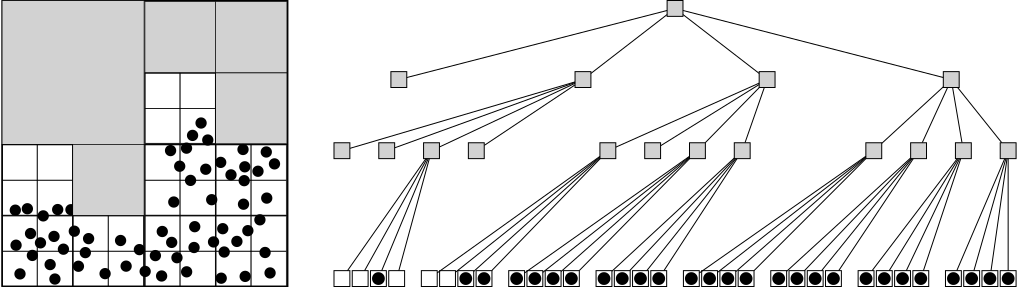
\includegraphics[width=\textwidth]{octree}
  \label{fig:octree}
  \caption[Funktionsweise eines Octrees]{Quadtree (2d-Äquivalent des Octrees) zur Veranschaulichung der Funktionsweise eines Octrees:
    Räumliche Unterteilung und deren die Baum-Darstellung.
    Rekursive Zerlegung der interessanten Zellen bis zur gewünschten Auflösung in Ebene 4, dann zellweises Binning der Atome.
  }
\end{figure}

\begin{algorithm}
  \begin{algorithmic}
%    \Input $root$ - Stammzelle des Octrees
%    \Input $i[3]$ - globale Adresse der Zielzelle
%    \Input $allocate$ - Ob die Zelle neu erstellt werden soll
    \Result null falls leer, sonst Zielzelle
    \State
    \Function{getcell-octree}{$cell, id, allocate$}
    \State $d \gets $\Call{depth}{root}
    \Comment{Relative Tiefe, an der sich die Zielzellen befinden}
    \If{$d = 0$}
    \State\Return cell
    \EndIf
    \If{not $cell.children$}
    \If{allocate}
    \State $cell.children \gets $new cell[8]
    \Else
    \State \Return null
    \EndIf
    \EndIf
    \State $childid \gets $\Call{bitand}{id[0], $2^{d-1}$}
    + $2\cdot$\Call{bitand}{id[1], $2^{d-1}$}
    + $4\cdot$\Call{bitand}{id[2], $2^{d-1}$}
%    \State \Comment{Indiziert die Subzelle aus der globalen Position}
    \State \Return\Call{getcell-octree}{$cell.children[childid], i, allocate$}
    \EndFunction
  \end{algorithmic}
  \caption[Zell-Addressierung in Octrees]{Rekursive Zell-Addressierung und -Allokierung im Octree: Bei jedem Schritt wird das Problem in 8 Unterzellen geteilt, woraus eine Laufzeit von \BigO{d}$=$\BigO{\log{c}} resultiert}
  \label{algo:octreeadressing}
\end{algorithm}

\todo[inline]{Wars das? Formeln?}

\subsection{k-d-Bäume}

Für Nachbarschafts- und Bereichssuchen wird wegen ihrer hervorragenden Suchkomplexität auf k-d-Bäume zurückgegriffen, die einen kartesischen Raum in orthogonale Zellen mit jeweils einem Atom unterteilen.
Es ergibt sich ein balancierter Binärbaum mit Atomen als Knoten, dessen Haupteigenschaft in impliziter Betrachtung von Abstandsrelationen liegt.
So lassen sich große Bereiche aus einer Abstandssuche oder Bereichssuche ausschließen, sobald ein Atom mit geringerem Abstand gefunden wurde.
Somit lässt sich per binärer Suche das nächste Atom eines beliebigen Punktes in \BigO{\log{n}} finden.
Sucht man $N$ Nächstnachbaratome, lassen sie sich durch Kombination mit einem Heap in \BigO{\log{n}\log{N_r}} finden, was zwar im Vergleich zu Octrees zu höheren asymptotischen Laufzeiten führt, jedoch zu kürzeren realen Laufzeiten führt.
\footnote{Vergleich dazu auch Heapsort vs. Quicksort: Cachingeffekte}
Aktualisierungen von Knoten behandelt man durch Standardalgorithmen wie Baumrotation in \BigO{\log{n}}.

Eine weitere Eigenschaft von k-d-Bäumen ist außerdem, dass sie nicht auf endliche Räume beschränkt sind und zuverlässig beliebig große Systeme beschreiben können.
Durch adaptives Neubalancieren erreicht man dennoch bei typischerweise einseitigem Schichtwachstum die oben erwähnten Suchlaufzeiten auf Kosten der Manipulationseffizienz.

\begin{figure}[bthp]
  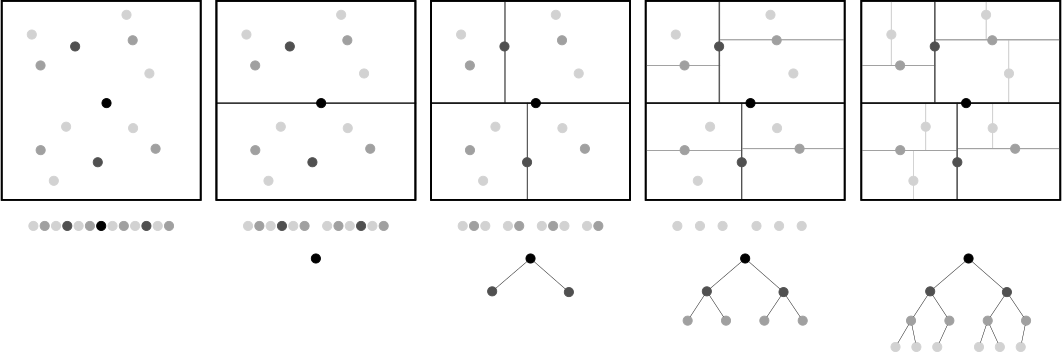
\includegraphics[width=\textwidth]{kdtree-tree}
  \caption[Konstruktion eines k-d-Baumes]{
    Rekursive Konstruktion eines k-d-Baumes: Die Punktmenge wird sortiert, der Median zum Baum hinzugefügt und seine Kinder aus den beiden Teilmengen per k-d-Baum-Konstruktion gewonnen.
    Der gewonnene Suchbaum ist effizient in Speicherplatz und Laufzeit der Suchoperationen.
  }
  \label{fig:kdtree}
\end{figure}

%% \begin{algorithm}
%%   \begin{algorithmic}
%%     \Input $points$ - Liste von Punkten
%%     \Input $k$ - Dimensionalität des Simulationsraumes
%%     \Result Root-Element eines vollständigen KD-Baumes aus diesen Punkten
%%     \State
%%     \Function{construct-kdtree}{$points, dim\gets0$}
%%     \State $n\gets$\Call{length}{points}
%%     \If{$n=0$}
%%     \State \Return null
%%     \Else
%%     \State \Call{sort}{$points, dim$} \Comment{Sortiert $points$ nach pos[$dim$]}
%%     \State $root\gets{}points\left[\lfloor\frac{n}{2}\rfloor\right]$
%%     \State $dim\gets(dim+1)\mod{k}$
%%     \State $root.left \gets$ \Call{construct-kdtree}{$points\left[0:\lfloor\frac{n}{2}\rfloor-1\right], dim$}
%%     \State $root.right \gets$ \Call{construct-kdtree}{$points\left[\lfloor\frac{n}{2}\rfloor+1:n-1\right], dim$}
%%     \State \Return $root$
%%     \EndIf
%%     \EndFunction
%%   \end{algorithmic}
%%   \caption[Konstruktion eines k-d-Baumes]{Rekursive Konstruktion eines k-d-Baumes (naive Implementierung)}
%%   \label{algo:kdtree-construction}
%% \end{algorithm}

Probleme von k-d-Bäumen zeigen sich bei der Suche nach einer Oberfläche einerseits und bei periodischen Räumen andererseits.
Die Oberfläche entlang einer Hauptachse lässt sich per Range Search mit anschließender Minimalsuche entlang der Suchachse effizient ermitteln, möchte man allerdings das Auftreffen eines Precursors mit beliebiger Inklination ermitteln, kann man auf keine optimale Methode zurückgreifen, sondern muss die Range Search auf einen größeren orthogonalen Suchbereich erweitern und darin eine Auswahl treffen.
Zudem führen lokale Aktualisierungen im schlimmsten Fall zur Neubalancierung des gesamten Baumes, wodurch die Betrachtung paralleler verzögerter Aktualisierungen erschwert wird.
Periodische Simulationsräume führen außerdem in der Nähe der Systemgrenze zu identischen Operationen auf periodischen Bildern des Baumes, die bei eventuellen Aktualisierungen ebenso weitreichende Restrukturierungen zur Folge haben.

Aus diesen Gründen lassen sich k-d-Bäume nicht zufriedenstellend im Parsivald-Modell nutzen.

\subsection{Delaunay-Triangulation}\label{datadelaunay}

\begin{figure}[bhpt]
  \centering
  \def\svgwidth{\textwidth}
  \input{img/delaunay.pdf_tex}
  \caption[Delaunay-Triangulation]{Beispiel der Konstruktion einer Delaunay-Triangulation (c) aus einer Punktwolke (a).
    Für jedes Simplex (hier 2d-Simplex, also Dreieck) muss das Delaunay-Kriterium eingehalten werden:
    Es dürfen sich keine weiteren Punkte im Umkreis des Simplices befinden (b).
  }
  \label{fig:delaunay}
\end{figure}

Eine alternative Partitionsmethode findet sich in Triangulationen, die die konvexe Hülle der Punktwolke raumfüllend in nichtüberlappende k-dimensionale Simplexe entsprechend einer weiterhin Delaunay-Kriterium genannten Beziehung zerlegen:
Im Umkreis eines Simplexes befinden sich keine weiteren Punkte aus der Punktwolke.
Damit ergibt sich eine Vielzahl an Eigenschaften, die für verschiedene Problemstellungen zu effizienten Lösungen führen.
So beinhaltet eine Delaunay-Triangulation als Subgraphen den Nächstnachbargraphen, die Alpha-Form und die konvexe Hülle, ist dual zum Voronoi-Diagramm und es lässt sich leicht auf Konnektivität prüfen.


\begin{itemize}
\item Jeder Punkt ist Eckpunkt eines oder mehrerer Simplexe
\item Simplexe überschneiden sich nicht
\item Im Umkreis eines Simplexes befinden sich keine weiteren Punkte
\item Die Vereinigung aller Simplexe ergibt die konvexe Hülle
\item Alpha-Form $\subset$ Delaunay-Triangulation
\item %Ein Punkt teilt sich mit seinem nächsten Nachbarn mindestens einen Simplex \\
  %$\Leftrightarrow$
  Nächstnachbargraph $\subset$ Delaunay-Triangulation
  %% \item Die Delaunay-Triangulation und das Voronoi-Diagramm über die selben Punkte sind dual\\
  %% $\Rightarrow$ Allgemeine Nachbarschaftssuche ist \BigO{k\log k}
\end{itemize}

Delaunay-Triangulationen werden somit für Oberflächenbetrachtungen interessant, da sie über die Alpha-Form, welche durch Auswahl der Punkte aller Simplexe mit Umkreisradien oberhalb einer stoffabhängigen Grenze ermittelt wird und die wahrgenommene Oberfläche eines Systems darstellt.
Somit lassen sich Oberflächenrauheiten, Nanoporen und bei extremen Grenzwerten auch Kristalldefekte bestimmen.
Mit wenig Mehraufwand gegenüber reinen Delaunay-Triangulationen ließen sich somit einerseits Auswertungen bei laufenden Simulationen durchführen und Prozesse gegebenenfalls direkt optimieren, andererseits ist die gesamte Oberfläche zur Simulation von Oberflächenereignissen bekannt und direkt parametrisiert.

\subsubsection{Algorithmen zur Konstruktion einer Delaunay-Triangulation}

Zur Delaunay-Triangulierung aus einer Punktmenge stehen verschiedene Algorithmen zur Verfügung, die auf unterschiedlichen Methoden aufbauen.

\begin{itemize}
\item Flip-basierte Algorithmen (Local Improvement)\\
  Man startet mit einer beliebigen Triangulation, prüft den Umkreis aller Simplexe auf enthaltene Punkte und korrigiert gegebenenfalls per Flip-Algorithmus, der in Abbildung \ref{fig:delaunay-flip} dargestellt ist.
  Diese Algorithmen konvergieren typischerweise in \BigO{n^2} und sind damit vergleichsweise langsam.

\item Scan-Algorithmus (Incremental Construction)\\
  Man konstruiert schrittweise Simplexe, die das Delaunay-Kriterium erfüllen und keine nachträgliche Änderung benötigen.
  Durch viele Vergleiche und Sortierungen varieren typische asymptotische Laufzeiten zwischen \BigO{n\log{n}} und \BigO{n^2}.

\item Einfügungs-Algorithmen (Incremental Insertion)\\
  Man erstellt einen beliebig großen Simplex, der die gesamte Punktmenge beinhaltet, und fügt schrittweise einzelne Punkte in die Triangulation ein.
  Der den eingefügten Punkt umfassende Simplex wird an ihm in mehrere Unter-Simplexe geteilt, auf den und dessen unmittelbare Nachbarn ein Flip-basierter Algorithmus ausgeführt wird.
  Laufzeiten sind typischerweise gering mit \BigO{n\log{n} + n^{\lceil d/2 \rceil}}.

\item Divide-and-Conquer-Algorithmen\\
  Man teilt die Punktmenge in Untermengen, die rekursiv trianguliert und anschließend an ihren Grenzen miteinander zur Zieltriangulation vereinigt werden.
  Hauptproblem ist die Vereinigung der Teiltriangulierungen, die in zwei Dimensionen aufgrund von Ordnungsrelationen entlang der Grenze beinahe trivial, in höheren Dimensionen jedoch mit Problemen verbunden ist.
  Eine mögliche Lösung ist der DeWall-Algorithmus\cite{cignoni_1998}, dessen Verknüpfungsoperation entlang der Grenzen teilperiodischer Räume interessant wird.
  In zwei Dimensionen erreicht man \BigO{n\log{n}}, höhere Dimensionen können per DeWall-Algorithmus mit einer Laufzeit von \BigO{n^{\lceil d/2 \rceil + 1}} behandelt werden, die sich jedoch nur in pathologischen Fällen zeigt.
  Nimmt man annähernde Gleichverteilungen an, konvergiert dieser Algorithmus in drei Dimensionen subquadratisch, man sollte jedoch betrachten, dass er sich gegenüber anderer Konstruktionsalgorithmen durch einfache Parallelisierung sowie der Möglichkeit der Aktualisierung großer Raumbereiche auszeichnet.

\item Höherdimensionale Einbettung\\
  Hier wird die Punktmenge in eine höhere Dimension transformiert, in der deren konvexe Hülle berechnet wird, die dann in den ursprünglichen Raum herunterprojiziert wird und darin eine gültige Delaunay-Triangulation ergibt.
  Dieser Algorithmus ist von rein akademischem Interesse, da Einfügungs-Algorithmen für allgemeine Fälle geringere Laufzeiten ermöglichen.
  Interessant wird diese Methode ebenfalls bei Hinzufügung und Aktualisierung von Punkten.

\end{itemize}

\subsubsection{Flip-Algorithmus}

\begin{figure}[bhpt]
  \captionsetup[subfigure]{singlelinecheck=false}{
    \def\subfigwidth{0.23\textwidth}
    \def\svgwidth{\textwidth}
    \begin{subfigure}[t]{\subfigwidth}
      \includegraphics[width=\textwidth]{delaunay-flip-a}
      \subcaption{Ausgangstriangulation}
      \label{fig:delaunay-flip-a}
    \end{subfigure}
    \hfill
    \begin{subfigure}[t]{\subfigwidth}
      \includegraphics[width=\textwidth]{delaunay-flip-b}
      \subcaption{Vereinigung invalider Simplexe}
      \label{fig:delaunay-flip-b}
    \end{subfigure}
    \hfill
    \begin{subfigure}[t]{\subfigwidth}
      \includegraphics[width=\textwidth]{delaunay-flip-c}
      \subcaption{Aufteilung in neue valide Simplexe}
      \label{fig:delaunay-flip-c}
    \end{subfigure}
    \hfill
    \begin{subfigure}[t]{\subfigwidth}
      \includegraphics[width=\textwidth]{delaunay-flip-d}
      \subcaption{Ergebnis}
      \label{fig:delaunay-flip-d}
    \end{subfigure}
  }
  \caption{
    Flip-Algorithmus: Invalide Simplexe werden aufgelöst und entlang einer neuen Grenze in neue Simplexe überführt.
    Diese Operation läuft in \BigO{k_d\log{k_d}} Prüfungen bei Aktualisierung der Punkte eines Simplexes, mit $k_d$ als oberer Schranke der Zahl der Simplexe eines Punktes.
  }
  \label{fig:delaunay-flip}
\end{figure}

Basis vieler Algorithmen auf Delaunay-Triangulationen basieren auf dem \textbf{Flip-Verfahren} (Abbildung \ref{fig:delaunay-flip}), mit dem unzulässige in zulässige Simplexe überführt werden.
Dabei werden Grenzen zu dem benachbarten Simplex, dessen Punkt innerhalb des Umkreises liegt, aufgelöst und aus den dann verfügbaren Punkten zwei neue Simplexe gebildet.
Im Anschluss ist es häufig notwendig, die neu entstandenen Simplexe sowie die ursprünglichen Nachbarn des zweiten Simplexes auf die gleiche Art zu prüfen.

%% Nachbarschaftssuche nicht notwendig

%% \subsubsection{Nachbarschaftssuche}
%% Für die Nachbarschaftssuche eines Referenzpunktes werden die raumfüllenden Eigenschaften der Triangulation relevant.
%% Der notwendigerweise konvexe, sonst aber beliebige Suchbereich um den Referenzpunkt wird von Simplexen überdeckt, die in direkter oder indirekter Nachbarschaft des Punktes liegen.
%% Somit teilen sich alle Punkte innerhalb des Suchbereiches eine Kante eines Simplexes mit einem anderen Punkt im Suchbereich, sofern der Suchbereich hinreichend groß ist.
%% Ausgehend vom Referenzpunkt sucht man entlang aller Kanten nach Punkten, die innerhalb des Suchbereiches liegen, bis alle potentiellen Punkte überprüft wurden.
%% Diese Vorgehensweise ist in Algorithmus \ref{algo:delaunay-neigbors} ausführlich beschrieben.

%% \begin{algorithm}
%%   \centering
%%   \begin{algorithmic}
%%     \State Result = \{\}
%%     \State Queue = \{ P$_0$ : P$_0 \in$ Volume \}
%%     \While{Queue $\neq \emptyset$}
%%     \State Sei P $\in$ Queue
%%     \State Queue = Queue $\setminus$ \{ P \}
%%     \If{P $\in$ Volume}
%%     \State Result = Result $\cap$ \{ P \}
%%     \State Queue $\cap$ (Neighbors(P) $\setminus$ Result)
%%     \EndIf
%%     \EndWhile
%%   \end{algorithmic}
%%   \caption[Nachbarschaftssuche auf einer Delaunay-Triangulation]{Nachbarschaftssuche auf einer Delaunay-Triangulation.
%%     Ist der Suchraum konvex und hinreichend groß, lässt sich damit effizient nach Nachbarn eines bestimmten Punktes suchen.
%%   }
%%   \label{algo:delaunay-neighbors}
%% \end{algorithm}

\subsubsection{Alpha-Form}

Die Alpha-Form (Abbildung \ref{fig:delaunay-alpha}) beschreibt anschaulich, aus welchen Punkten, Linien und Flächen die Oberfläche einer Punktmenge besteht.
Im Gegensatz zur konvexen Hülle kann sie auch Einschlüsse, Poren und Oberflächenrauheiten je nach Wahl des $\alpha$-Wertes darstellen.
Allgemeine Hüllen von Triangulationen werden dabei als Vereinigung der Menge genau der Flächen gewonnen, die nur einem Simplex zugeordnet sind, so dass man die konvexe Hülle beispielsweise als Hülle einer Delaunay-Triangulation erhält.
%% Abhängig vom Anwendungsfall lassen sie sich als Menge von Punkten, Verbindungslinien oder Flächen ausdrücken.

Für die Konstruktion von Alpha-Formen aus Delaunay-Triangulationen gibt es dabei zwei äquivalente Ansätze:
Einerseits kann man alle Simplexe mit einem Umkreisradius $r_d > \alpha^{-1}$ aus der Delaunay-Triangulation entfernen und die Hülle der so entstandenen Triangulation bilden.
Andererseits kann man alle Simplexe mit einem Umkreisradius $r_d > \alpha^{-1}$ aus der Delaunay-Triangulation auswählen und deren Hülle bilden.
Die Nutzung des $\alpha$ als inversen Parameter ergibt sich hierbei aus weitergehenden Überlegungen, die konvexe Hülle als $\alpha=0$ und Tests mit invertierten Kreisflächen als $\alpha<0$ darzustellen.

Beide Methoden erzeugen dabei leicht unterschiedliche Ergebnisse:
Ansatz 1 garantiert, dass die so entstandenen Oberflächen aus Simplexen aufgebaut sind, also keine einzelnen Punkte oder Dreiecke beinhalten und somit eines oder mehrere Volumen beschreiben.
Ansatz 2 erzeugt in erster Linie die gleiche Oberfläche, erfasst allerdings zusätzlich innerhalb der Auswahl auch einzelne Atome, Verbindungslinien oder Flächen, die keinem Volumen zugeordnet sind und somit im atomistischen Kontext einzelne Atome oder kleine Moleküle darstellen.
Um beim zweiten Ansatz auch Elemente der konvexen Hülle erfassen zu können, wird die Triangulation häufig innerhalb und inklusive der Eckpunkte eines unendlichen virtuellen Simplexes vorgenommen, wie es auch bei einigen Konstruktionsmethoden üblich ist.
Per Konnektivitätsprüfung der Oberflächendreiecke lässt sich zwischen zusammenhängenden Oberflächen, Einschlüssen und eigenständigen Punkten unterscheiden.

In der Anwendung werden Alpha-Oberflächen für die Bestimmung von Rauheiten von Oberflächen oder Volumen poröser Materialien interessant, da sie sich als Punktmengen- beziehungsweise Polygonoperationen gestalten.
Für Simulationen von Oberflächenabscheidungen ließen sich auf diese Weise auch Bedeckungen mit Precursorliganden ermitteln.

\begin{figure}[bhpt]
  \centering
  \captionsetup[subfigure]{singlelinecheck=false}{
    \def\subwidth{0.4\textwidth}
    \def\svgwidth{\textwidth}
    \begin{subfigure}[t]{\subwidth}
      
\includegraphics[width=\textwidth]{delaunay-alpha-a}
      \subcaption{Delaunay Triangulation einer beliebigen Punktmenge}
      \label{fig:delaunay-alpha-a}
    \end{subfigure}
    \hfill
    \begin{subfigure}[t]{\subwidth}
      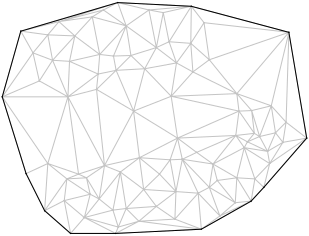
\includegraphics[width=\textwidth]{delaunay-alpha-b}
      \subcaption{Konvexe Hülle: Hülle der Triangulation}
      \label{fig:delaunay-alpha-b}
    \end{subfigure}
  }
  \vspace{2em}
  \captionsetup[subfigure]{singlelinecheck=false}{
    \def\subwidth{0.4\textwidth}
    \def\svgwidth{\textwidth}
    \begin{subfigure}[t]{\subwidth}
      \includegraphics[width=\textwidth]{delaunay-alpha-c}
      \subcaption{Alpha-Form: Hülle nach Entfernung von Simplexen mit $r_d > \alpha$}
      \label{fig:delaunay-alpha-c}
    \end{subfigure}
    \hfill
    \begin{subfigure}[t]{\subwidth}
      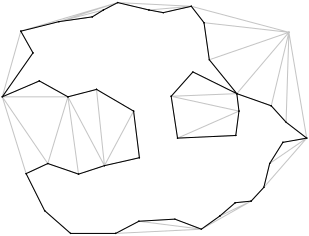
\includegraphics[width=\textwidth]{delaunay-alpha-d}
      \subcaption{Alpha-Form: Hülle nach Entfernung von Simplexen mit $r_d < \alpha$ (nur innen)}
      \label{fig:delaunay-alpha-c}
    \end{subfigure}
  }
  \caption[Methoden zur Bestimmung der Oberfläche per Delaunay-Triangulation]{Verschiedene Methoden zur Bestimmung der Oberfläche per Delaunay-Triangulation. Man beachte, dass die in (d) genutzte Methode den Ausreißer-Punkt oben rechts mit trianguliert, jedoch nicht zur Oberfläche zählt, da für keinen seiner Simplexe $r_d < \alpha$ gilt}
  \label{fig:delaunay-alpha}
\end{figure}

\clearpage
\input{prerequisites}

  \cleardoublepage
  \chapter{Methoden und Modelle}
\label{models}
%% \chapter{ReaxFF-Potentiale für SiO$_2$-Abscheidungen}

\todoline{Kurze Einleitung}

\section{Überblick über bisherige Methoden}

In der Vergangenheit wurden reine molekulardynamische und kinetische Monte Carlo-Methoden wiederholt zur Simulation von verschiedenen Aspekten von Gasphasenabscheidungen zu Rate gezogen.
Im Folgenden soll ein Überblick über die bisherigen Untersuchungen gegeben werden.

\subsection{Bisherige KMC-Simulationen}

\subsubsection{Dwivedi: gitterbasierte 2D-ALD}

\textsc{V. Dwivedi} und \textsc{A. Adomaitis} haben ein zweidimensionales KMC-Modell für \ce{Al2O3}-ALD entwickelt\cite{dwivedi_multiscale_2009,dwivedi_multiscale_2009-1,dwivedi_multiscale_2010}, um den Gasverbrauch und den GPC-Wert in Abhängigkeit der Partialdrücke der Precursorgase zu ermitteln und in eine Gasflusssimulation zur Kontrolle des Durchmessers von Mikroporen einzubinden.
Dazu werden die Plätze eines hexagonalen Gitters auf die Spezies Sauerstoff, Hydroxyl und Aluminium aufgeteilt, Zustandsübergänge in Abhängigkeit der 6 Nachbarzellen definiert und Übergangsraten ausgehend von den Energiebarrieren der entsprechenden chemischen Reaktionen ermittelt.
Aussagen über die Schichthöhe ergeben sich über die Festlegung des vertikalen Gitterabstandes anhand der Einheitszelle eines \ce{Al2O3}-Kristalles mit anschließender vertikaler Oberflächensuche.

Damit lassen sich zwar GPC-Werte und Precursorverbrauch annähernd bestimmen, doch ist keine strukturelle Aussage möglich, obwohl elegant gewählte Ereignisse die \ce{Al2O3}-Stöchiometrie erzwingen.
%% Tests des Modelles schlugen zudem häufig fehl, da das System eine Tendenz zur Bildung von \ce{Al-O}-Ketten und zur Verstärkung von Kratern hat, wobei die Ursache nicht klar dem eigenen Code oder dem Dwivedi-Modell zuzuordnen ist.

\subsubsection{Mazaleyrat: gitterbasierte 3D-ALD}

Ähnlich zum Dwivedi-Modell nutzt auch das Modell von \textsc{Mazaleyrat et al.}\cite{mazaleyrat_methodology_2005} ein Simulationsgitter, das aber über drei Dimensionen definiert ist, auf dem \ce{MgAl2O4}-Spinell-basiert und als Annäherung der eigentlichen Atompositionen verstanden wird.
Durch geschickte Indizierung des Gitters wird eine effiziente Methode geschaffen, \ce{Al2O3} in KMC-Simulationen aufzuwachsen, deren strikt kristalline Repräsentation die eigentlich amorphe Struktur eigentlich nicht darstellen kann, obwohl das Ziel des Modelles in der Abscheidung von Dielektrika auf Silizium-Substraten liegt.
Von den Autoren wurde keine Betrachtung der Rauheit, des Besetzungsgrades der Gitterplätze oder des Wachstumsverhaltens jenseits des dritten Schrittes veröffentlicht.

\subsubsection{Stamatakis: Oberflächen-Reaktionen mit Zacros}

Zwar handelt es sich beim Zacros-Modell von der Forschergruppe um \textsc{M. Stamatakis}\cite{stamatakis_graph-theoretical_2011,nielsen_parallel_2013,stamatakis_zacros_2014} um eine zweidimensionale Oberflächenbeschreibung für katalytische Reaktionen, doch liegt nahe, seinen effizienten graph-basierten Suchansatz für Ereignisse auch für Gasphasenabscheidungen nutzen zu wollen.
Die Besonderheit von Zacros liegt in einer vereinheitlichten Formulierung der lokalen Zustände und Zustandsübergänge als Teilgraphen des Simulationsgitters, welche effizient durch Algorithmen zum Teilgraphen-Vergleichs überprüft werden können.
Ergänzt durch quantenmechanische Simulationen für die Bestimmung der Reaktionsraten, ergibt sich ein wertvolles Werkzeug zur stochastischen Simulation der Reaktionskinetik von Oberflächenprozessen.
Aufgrund seiner Formulierung ist aber auch Zacros auf ein periodisches Simulationsgitter begrenzt, welches durch seine Beschreibung als Graph jedoch aus beliebig geformten Einheitszellen bestehen kann.

\subsection{Bisherige MD-Simulationen}

Molekulardynamische Simulationen werden seit vielen Jahrzehnten zur Bestimmung struktureller und thermodynamischer Eigenschaften verschiedener Materialien eingesetzt, aber nur selten zur Beschreibung von Gasphasenabscheidungen.
Sie lassen sich aber zur Beschreibung von Teilaspekten nutzen, wofür meist durch die Simulation periodischer Strukturen Rückschlüsse auf bestimmte Eigenschaften gezogen werden.

\subsubsection{Gold}
\textsc{Chamati et al.}\cite{chamati_second-moment_2004} haben das thermische Verhalten von Gold-Bulks untersucht, wo hingegen \textsc{Chui et al.}\cite{chui_molecular_2007}, \textsc{Liu et al.}\cite{liu_melting_2001} und \textsc{Shim et al.}\cite{shim_molecular_2003} strukturelle und thermodynamische Eigenschaften von Gold-Nanoclustern betrachtet haben.
Veröffentlichungen zu MD-Simulationen von Aspekten der Gold-PVD finden sich ebenfalls vereinzelt, doch simulieren die meisten den Einschlag von Edelgas-Ionen auf dem Target mit Energien von \SIrange{1}{400}{\kilo\electronvolt}\cite{insepov_molecular_1995,shapiro_simulation_1999} oder tragen komplette Cluster statt einzelner Atome auf\cite{inoue_molecular_2008}.

\subsubsection{Kupfer und Nickel}
Kupfer-Nickel-Multilagensysteme wurden unter anderem von \textsc{Foiles et al.}\cite{foiles_calculation_1985} simuliert, wobei der Einfluss der Sputterenergie der Atome auf die Rauheit der abgeschiedenen Oberflächen und Schichten hauptsächlich von \textsc{Zhou et al.}\cite{zhou_atomistic_1998} untersucht wurde.
Der durch unterschiedliche Bindungslängen entstehende Versatz zwischen den Kupfer- und Nickel-Kristallen wurde von \textsc{Rao et al.}\cite{rao_atomistic_2000} simuliert.

\subsubsection{Silizium}
Für Silizium finden sich thermodynamische Expansions-Simulationen von \textsc{Buda et al.}\cite{buda_thermal_1990} sowie Untersuchungen von \textsc{Insepov et al.}\cite{insepov_molecular_1995} zur Auswirkung von gerichteten Cluster-Einschlägen in Abhängigkeit der Einschlagsenergie.
\todo[inline]{mehr! PVD und Oxidation / Hydroxylierung von Oberflächen}

\subsubsection{Aluminiumoxid}
Für amorphe und kristalline \ce{Al2O3}-Bulks finden sich Simulationsergebnisse von \textsc{Alvarez et al.}\cite{alvarez_computer_1995,alvarez_molecular_1992} und von \textsc{Gutierrez et al.}\cite{gutierrez_molecular_2002} sowie für \ce{Al2O3}-Oberflächen von \textsc{Adiga et al.}\cite{adiga_atomistic_2006}.
Sowohl Schmelzen als auch amorphes \ce{Al2O3} wurden unter anderem von \textsc{Gutierrez et al.}\cite{gutierrez_structural_2000} und \textsc{Vashishta et al.}\cite{vashishta_interaction_2008} simuliert.
\textsc{Russo et al.}\cite{russo_molecular_2011} haben erfolgreich Oberflächen-Reaktionen zwischen einem Aluminium-Cluster und Wassermolekülen unter Nutzung der ReaxFF-Formulierung simuliert, während \textsc{Puri et al.}\cite{puri_thermo-mechanical_2010} das Schmelz- und Diffusionsverhalten von \ce{Al2O3}-ummantelten \ce{Al}-Nanopartikeln untersuchten.
Diese Vielfalt an Simulationen zeigt sich jedoch nicht in der Zahl der veröffentlichten Potentialparametrisierungen, von denen nur eine kleine Zahl für \ce{Al2O3}-Simulationen zur Verfügung stehen.

\subsubsection{Fazit}
Die Untersuchungen beschränken sich meist auf \num{<10000} Atom, wodurch sich insbesondere bei der Bestimmung struktureller Eigenschaften Finite Size-Effekte bemerkbar machen können.
Darüber hinaus werden einige der genutzten Potentialparametrisierungen nicht veröffentlicht, wodurch die entsprechenden Ergebnisse nicht reproduzierbar oder auf andere Probleme übertragbar sind.
Dem steht die Vielzahl von verschiedenen Parametrisierungen gegenüber, von denen jede einzelne nur auf ein spezielles Problem anwendbar ist.
Eine Suche nach EAM-Kraftfeldern für Kupferatome in der Potentialdatenbank der NIST\cite{becker_interatomic_2014} ergibt beispielsweise eine zweistellige Zahl an Kupfer-Parametrisierungen, die einzeln hinsichtlich eigener Problemstellungen überprüft werden müssen (Abschnitt \ref{copperpvd}).

\subsection{Zielsetzung für Parsivald}

Das nachfolgend vorgestellte Parsivald-Modell soll die Stärken beider Simulationsmethoden vereinen, um so Gasphasenabscheidungen in großen Simulationsräumen mit atomistischer Genauigkeit simulieren zu können.
Dabei sollen Substrate einer Größe von \SI{10x10}{\nano\meter} bis \SI{1x1}{\micro\meter} und Schichtwachstum über \SI{100}{\nano\meter} (\num{1000} ALD-Zyklen) in \SI{8}{\hour} bis \SI{3}{\week} berechnet werden können, wobei \num{2e9} Atome erreicht werden können.

\clearpage
\section{Parsivald-Modell}
\label{sec:parsivald}

\subsection{Beschreibung}

\todo{subsubsections}

Parsivald ist der Name eines Modelles mit gleichnamiger Implementierung, das unter Kombination von Kinetic Monte Carlo-Methoden mit molekulardynamischen Berechnungen Oberflächenwachstum auf großen Substraten effizient simulieren kann.

\begin{figure}[tbh]
  \centering
  \def\svgwidth{\textwidth}
  \input{img/parsivald-schema-flat.pdf_tex}
  \caption[Parsivald-Schema]{
    Auswahl und Durchführung eines Oberflächenereignisses, verteilt auf KMC und MD.
  }
  \label{fig:parsivald-schema}
\end{figure}

Dazu wird der gesamte Wachstumsprozess in das Auftreffen eines Precursormoleküles oder Atomes und seine Reaktion beziehungsweise physikalische Anlagerung an der Oberfläche getrennt.
Für alle weiteren Prozesse wurden folgende Annahmen getroffen:

\begin{enumerate}
\item Alle Reaktionen finden auf der Oberfläche statt
\item Reaktionen sind zeitlich und räumlich getrennt
\item Oberflächendiffusion ist vernachlässigbar
\item Bulkdiffusion ist vernachlässigbar
\end{enumerate}

Reaktionen in der Gasphase sind also ebenso wenig darstellbar wie diffusionsgestützte Prozesse.
Ohne diese notwendigen Annahmen käme das Parsival-Modell einer reinen Molekulardynamik-Simulation gleich.
Stattdessen werden Reaktionen auf folgende Weise modelliert:

Auf der Oberfläche des gesamten Simulationsraumes wird zuerst nach einem Ort für eine Precursorreaktion gesucht.
Dessen Auswahl kann rein zufällig sein, oder aber von der lokalen Nachbarschaft abhängen, beispielsweise über molekulare Gruppen oder Atomdichten.
Nach dessen Auswahl extrahiert man alle Atome in der unmittelbaren Nachbarschaft und erstellt aus ihnen eine Reaktionszelle für MD-Simulationen.
Diese Zelle enthält einen Rand fester Atome, dessen Größe wie auch die Größe der Zelle selbst von der Reichweite der genutzten MD-Potentiale abhängt.
In diese Zelle fügt man je nach Simulationsart, gewünschter Genauigkeit und Fähigkeit der Potentiale das Precursormolekül oder einzelne Atome daraus ein.
Nach einer erfolgreichen Reaktions- oder Relaxationssimulation fügt man die Atome der Reaktionszelle wieder in die Gesamtstruktur ein und wählt das nächste Oberflächenereignis aus.

Ergänzend lässt sich durch verschiedene Optimierungen die Laufzeit minimieren.
Beispielsweise kann man durch Parallelisierung des KMC-Teiles linearen Speedup \todo{Linearer Speedup?} erreichen, der nur durch die Größe des Raumes begrenzt ist.
Eine Parallelisierung der MD-Simulationen ist hingegen nicht sinnvoll, da bloß kleine Mengen von maximal einigen Tausend Atomen gleichzeitig simuliert werden.
Andererseits kann man durch oben diskutierte Datenstrukturen die Suche neuer KMC-Ereignisse sowie die Extraktion einer atomaren Nachbarschaft verkürzen.

\todo{fehlt noch was?}

\subsection{Einschränkungen}

Neben den durch die oben genannten Annahmen \todo{Referenz} eingeführten gibt es noch eine weitere Einschränkung.
So lassen sich nur Prozesse und Strukturen betrachten, die auch durch Molekulardynamik darstellbar sind, wobei sich sowohl das Bulk-Material als auch seine Oberfläche simulieren lassen müssen.
Im optimalen Fall stellen die genutzten MD-Potentiale auch noch Precursor-Oberflächen-Reaktionen verlässlich dar, so dass man auf weitere Annäherungen verzichten kann.
Darunter fallen die Reduktion des Precursors auf sein Zentralatom, explizite sterische Hinderung sowie eine ausführliche Vorauswahl der Reaktionsorte.

Falls sich der komplette Precursor oder seine Reaktion mit der Oberfläche nicht durch passende MD-Potentiale darstellen lässt, kann man auf die Abscheidung seines Zentralatomes zurück greifen.
Obwohl es sich um eine stark vereinfachte Methode einer chemischen Abscheidung handelt, lässt sich so wenigstens das Wachstum der Struktur beobachten.
Da sich so keine Hinweise auf zurück gebliebene Precursorliganden auf der Oberfläche finden, muss man zusätzlich die sterische Hinderung explizit modellieren, um freies Wachstum zu verhindern.

\missingfigure{steric-hindrance}

Sterische Hinderung verhindert normalerweise durch die lokale Oberflächendichte von Precursorliganden eine weitere Anlagerung von Precursormolekülen bei chemischen Abscheidungen, bis diese Liganden wieder von der Oberfläche entfernt wurden.
Als Ersatz wird eine kugelförmige Zone definiert, innerhalb derer weitere Precursorreaktionen auf der Oberfläche ausgeschlossen sind, bis der nächste Prozessschritt gestartet wurde.
Als entsprechender Parameter steht nun jedem möglichen Abscheidungsereignis der Radius dieser Kugel zur Verfügung.
Diese Methode ignoriert Feinheiten wie die genaue Anzahl an verbliebenen Precursorliganden, stellt jedoch eine gute\todo{wirklich gut?} Näherung dar.

\subsection{Implementierung}

Das Parsivald-Modell wurde ursprünglich im Rahmen meiner Bachelorarbeit \todo{Referenz} in Software umgesetzt.
Seither wurden verschiedene Funktionen ergänzt, wie beispielsweise Erleichterungen im Prozessdesign sowie der separate PVD-Modus.
Auch einfachere Möglichkeiten, eine bestimmte Zahl an Worker-Prozessen zu starten, vereinfacht die Nutzung der Software auf größeren Clustersystemen.

Grundlage der Implementierung bieten hauptsächlich die beiden Bibliotheken libenskmc sowie LAMMPS für KMC und MD, wobei libenskmc aus eigener Entwicklung stammt.
Man hätte an dieser Stelle auch die SPPARKS-Bibliothek für KMC-Simulationen einbinden können, die von den selben Autoren der LAMMPS-Bibliothek stammt.
Es hat sich jedoch heraus gestellt, dass SPPARKS nur unter großem Aufwand das Parsivald-Modell handhaben könnte, was vor allem in Hinblick auf häufige kritische Abbrüche der LAMMPS-Bibliothek nicht vertretbar war.

Auf eigenen Code wurde bei folgenden Systemen gesetzt:
Das Host-Worker-System mit angebundenen Netzwerk-Code musste geschrieben werden, da LAMMPS die Nutzung einer MPI-Bibliothek unterbindet.
Die Octrees zum räumlichen Binning wurden eng mit libenskmc verzahnt, weshalb auf eine externe Geometrie-Bibliothek verzichtet wurde.
DUMP-Substrate werden aufgrund der klaren Format-Definition durch eigenen Code eingelesen.
Ebenso erfolgt die Ausgabe der .xyz-Dateien über eigenen Code.
Im Gegensatz dazu werden .lmp-Substrate jedoch über lmpio eingelesen, einer IO-Bibliothek für .lmp-Dateien, die im Hintergrund LAMMPS nutzt, um Kompatibilität mit der Vielzahl an uneindeutigen Atomeigenschaften zu garantieren.
Um Konformität zwischen Kommandozeilenargumenten und Konfigurationsdateien zu garantieren, wurde auf die ArgumentParser-Bibliothek zurück gegriffen, die aus eigener Feder entstammt und in weiteren externen Projekten Verwendung findet.
Die Abhängigkeitsauflösung bei KMC-Ereignissen entstammt ebenfalls der eigenen Feder, ebenso wie der sonstige Binding Code zwischen LAMMPS und libenskmc, inklusive beider Parallelisierung-Codes (Threads und losgelöste Unterprozesse).


\clearpage
\section{MD-Simulationen: Methoden und Auswertungen}
\label{mdmethods}

Dieser Abschnitt soll eine Übersicht über die molekulardynamischen Vorgehensweisen geben, welche im folgenden Kapitel~\ref{results} zur Anwendung kommen.
Diese Methoden werden für die Präparation von Strukturen, deren thermische und strukturelle Untersuchung sowie innerhalb der Parsivald-Simulationen selbst eingesetzt.

\subsection{Zeitskalen in MD-Simulationen}

MD-Simulationen werden maßgeblich durch den Zeitschritt $\Delta t$, die Thermostatdämpfung $\tau$, die Barostatdämpfung $\tau_p$ und die Relaxationszeit $t_\text{relax}$ bestimmt, welche systemabhängige Maximalwerte nicht überschreiten dürfen.
$\Delta t$ ist so zu wählen, dass schnelle Bewegungen nur geringe numerische Fehler verursachen, wofür je nach Art des numerischen Integrators mindestens \SI{20}{\percent} der Periodendauer der schnellsten Schwingung als Richtwert angenommen wurde.

$\tau$ und $\tau_p$ sollten groß genug gewählt werden, um zwischen den Zeitschritten nur geringe Änderungen vorzunehmen, da sonst die Dynamik des Systems gestört wird.
Typische Werte sind $\tau = 100 \Delta t$ und $\tau_p = 1000 \Delta t$.
Die Relaxationszeit $t_\text{relax}$ muss zuletzt oberhalb der vom Thermostat und von Barostat erzeugten Oszillationen der Temperatur und der Dichte liegen.

\subsection{Relaxierungen}

Ausgehend von einer präparierten Struktur wird das System auf die Relaxationstemperatur erwärmt, dort im kanonischen Ensemble für die Relaxationsdauer simuliert und bei Bedarf wieder auf eine Zieltemperatur abgekühlt.
Erwärmung und Abkühlung sind zwar optional, allerdings bei einigen Strukturen zur Reduktion numerischer Fehler notwendig, wie etwa zur Wahrung der Anschlussbedingungen der MD-Simulationen innerhalb von Parsivald.
Vergleiche zwischen Parsivald und reinen MD-Simulationen sollen die Ähnlichkeit der abgeschiedenen Strukturen prüfen, um Fehler aufgrund der gewählten Temperaturen zu vermeiden.

\subsection{Strukturanalysen}

Zur Auswertung einer Struktur bietet sich zuerst eine visuelle Beurteilung an, die mit entsprechenden Visualisierungsprogrammen vorgenommen werden kann.
Im Anschluss können die Dichte, Radiale Verteilungsfunktion, Bindungslänge und Koordinationszahl bestimmt werden, um die Struktur weiter zu charakterisieren und Aussagen über Kristallbildung treffen zu können.
Bei Kristallen kann eine Alpha-Form (Abschnitt~\ref{dataalphaform}) mit einem $\alpha$-Wert knapp oberhalb der Bindungslänge genutzt werden, um Fehlstellen im Gitter oder Gitterversetzungen zu identifizieren.

\subsection{Bestimmung der Dichte und Temperatur}

Zur Bestimmung der Dichte des Blocks eines amorphen Materials stehen verschiedene Möglichkeiten zur Verfügung, die letztendlich alle auf Zählung der Atome innerhalb eines begrenzten Volumens zurückgeführt werden können.
Da das Volumen des Simulationsraumes im isotherm-isobaren Ensemble durch das Barostat oszilliert, muss sie zeitlich über einen größeren Zeitraum als die Dämpfungskonstante $\tau_p$ gemittelt werden, da sie sonst nicht über die gesamte Periode der Oszillation betrachtet wird.

Ebenso muss zur Bestimmung der Temperatur auf das Konvergenzverhalten des Thermostates geachtet werden.
Die Temperatur wird aus dem Mittelwert der kinetischen Energie aller Teilchen bestimmt, welche jedoch schwanken kann, weshalb wiederum die Bildung eines Zeitmittelwertes notwendig wird.

\subsection{Radiale Verteilungsfunktionen, Bindungslänge und Koordinationszahl}

Die Radiale Verteilungsfunktion (RDF) $g_{\alpha\beta}(r)$ zweier Atomsorten $\alpha$ und $\beta$ ergibt sich als Histogramm der Zahl der Atome $n_{\alpha\beta}(r)$ in Abhängigkeit des Abstandes $r$, gewichtet über die Volumen der Bins, welche durch die radiale Beschreibung die Form von Kugelschalen annehmen.
\begin{equation}
  g_{\alpha\beta}(r) = \frac{1}{\rho_\alpha} \frac{d n_{\alpha\beta}(r)}{4 \pi r^2 dr} ~~,\quad \rho_\alpha = \frac{N_\alpha}{V}
\end{equation}
Ihr erstes Maximum bildet die Bindungslänge, während das Integral bis zur Koordinationslänge (erstes Minimum nach der Bindungslänge) die erste Koordinationszahl ergibt.
An der RDF-Darstellung lässt sich außerdem die strukturelle Ordnung erkennen:
RDF von perfekten Kristallen bestehen ausschließlich aus Spitzen an den Gitterpunkten, die auch für große Abstände noch klar erkennbar sind.
Bei amorphen Materialien hingegen konvergiert die Funktion schnell gegen den Grenzwert von 1, der anzeigt, dass keine langreichweitige Ordnung mehr vorhanden ist.

Beispiele radialer Verteilungsfunktionen finden sich in Abbildungen~\ref{fig:siliconresults-b},~\ref{fig:kulkarnirdf} und~\ref{fig:amorphousrdf}.

\subsection{Oberfläche, Schichtdicke, Rauheit und Porösität}
\label{mdmethods-surface}

Zur Bestimmung der Schichtdicke, Oberflächenrauheit oder Porösität muss zuerst die Oberfläche einer Schicht aus der Alpha-Form mittels Delaunay-Triangulation in Form einer Punktwolke bestimmt werden (Abschnitt~\ref{datadelaunay}).
Im Anschluss lässt sich aus der entstandenen Punktwolke der tiefste und höchste Punkt der Oberfläche sowie die Spannweite in z-Richtung bestimmen und durch Bildung des Mittelwertes die mittlere Schichtdicke ermitteln.
Durch Zählung der chemischen Elemente in der Punktwolke lässt sich zudem die Bedeckung der Oberfläche mit chemischen Gruppen bestimmen.
Durch Begutachtung der Oberflächen können außerdem Rückschlüsse auf die Porösität gezogen werden, indem neben der eigentlichen Oberfläche auch sämtliche Poren und Hohlräume innerhalb der Struktur aus der Alpha-Form gelesen werden.

\subsection{Reaktionen und Stabilität von Molekülen}

Einzelne oder mehrere Precursormoleküle werden mit externer Software (Materials Studio\cite{biovia_materials_2014} und Packmol\cite{martinez_packmol:_2009}) präpariert, mit Geschwindigkeiten im Rahmen der Zieltemperatur versehen und im mikrokanonischen Ensemble im Vakuum simuliert, um Aussagen über ihre Stabilität zu erhalten.
Diese wird bei einzelnen Datensätzen manuell durch Begutachtung der dynamischen Eigenschaften und der entstandenen Moleküle ermittelt, bei vielen Datensätzen wird eine automatische Auswertung auf Konnektivität der Atome durchgeführt, wodurch Aussagen über die entstandenen Moleküle getroffen werden können.
Die gleichen Untersuchungen geben Aufschluss über den Erfolg einer Reaktion.



  \cleardoublepage
  \cleardoublepage
\chapter{Ergebnisse}

Im Verlauf der Erforschung möglicher Prozesse wurden Abscheidungen verschiedener Materialien und Methoden simuliert, die unterschiedliche Aspekte der Präparation, Durchführung und Einschränkungen von Parsivald-simulierten Prozessen demonstrieren.

Abschnitt \ref{goldpvd} zeigt allgemeine Vorbetrachtungen eines Potentiales und seiner MD-Parameter sowie die Nutzung strukturierter Substrate anhand von Gold-PVD.
Im darauf folgenden Abschnitt \ref{copperpvd} werden verschiedene Potentiale auf die Anwendbarkeit auf Kupfer-PVD überprüft.
Per PVD abgeschiedene Multilagensysteme stehen in Abschnitt \ref{multilayer} \todo{phrasing}zur Untersuchung.
Silizium-PVD stellt abschließend Probleme mit amorphen Materialien in Abschnitt \ref{siliconpvd} dar.
%% Abschnitt \ref{silicacvd} demonstriert binäre Abscheidungssysteme anhand von Siliziumoxid-CVD.
%% Schließlich wird in Abschnitt \ref{aluminaald} ein ALD-Prozess anhand des TMA-\ce{H2O}-Prozesses untersucht.

\section{Gold-PVD}

Als Testsystem für PVD-Prozesse bietet sich Gold als ein System an, dessen Abscheidungsprozess zwar durch Oberflächendiffusion dominiert wird, jedoch kristalline Strukturen bildet und für das ausgiebig erforschte MD-Parametrisierungen existieren.

\subsection{Voruntersuchungen}

Als kristallines, unäres Abscheidungssystem wurden zur Vorbetrachtung die Bindungslängen, Dichten sowie Koordinationen der kristallinen Phase untersucht\todo{Oberfläche?}.
Eine Stabilitätsanalyse des Precursormoleküles entfällt, da bei PVD-Prozessen nur einzelne Atome auf die Oberfläche aufgebracht werden.
Die Ergebnisse dieser Untersuchungen, die erwartungsgemäß gute Übereinstimmung zwischen Simulation und Experiment zeigen, sind in Tabelle \ref{tab:goldpreresults} zusammengefasst.

\begin{table}[hbtp]
  %% \rowcolors{0}{white}{lightgray} 
  \caption[Eigenschaften von Gold]{Eigenschaften von Gold als Voruntersuchung des PVD-Prozesses. Die Abweichung der Koordinationszahl wird in der Nichtperiodizität der untersuchten Struktur vermutet}
  \label{tab:goldpreresults}
  \begin{tabularx}{\textwidth}{|XXXX|}
    \hline
    \textbf{unters. Größe} & \textbf{Simulation} & \textbf{Experiment} & \textbf{Abweichung}\\
    \hline
    Bindungslänge & 2.879 \AA & 2.884 \AA & 0.2\% \\
    Koordination & 11.81 & 12.00 & 1.6\% \\
    Dichte (300K) & 18.99 g/cm$^3$ & 19.30 g/cm$^3$ & 1.6\%\\
    Dichte (500K) & 18.89 g/cm$^3$ & 19.13 g/cm$^3$ & 1.2\%\\
    \hline
  \end{tabularx}
\end{table}


\subsection{Prozess-Simulation}

Mangels chemischer Reaktionen genügt es, die Auftrefforte der Goldatome zufällig gleichverteilt auf der xy-Ebene auszuwählen.

\subsubsection{Strukturierte Substrate}

Als nächste Stufe wurden strukturierte Substrate untersucht, von denen eine Auswahl in Abbildung \ref{fig:goldsubstrate} dargestellt sind.
Diese wurden per Materials Studio präpariert, per Atomsk in ein kompatibles Format überführt und anschließend von Parsivald eingelesen und mit einzelnen Goldatomen beschichtet.

\begin{figure}[bt]
  \captionsetup[subfigure]{singlelinecheck=false}
  \def\subfigwidth{0.31\textwidth}
  \begin{subfigure}[t]{\subfigwidth}
    \includegraphics[width=\textwidth]{Au_substrate_flat}
    \subcaption{Flaches Gold-Substrat}
    \label{fig:goldsubstrate-a}
  \end{subfigure}
  \hfill
  \begin{subfigure}[t]{\subfigwidth}
    \includegraphics[width=\textwidth]{Au_substrate_step30}
    \subcaption{Gold-Stufe, 30°}
    \label{fig:goldsubstrate-a}
  \end{subfigure}
  \hfill
  \begin{subfigure}[t]{\subfigwidth}
    \includegraphics[width=\textwidth]{Au_substrate_tip60}
    \subcaption{Gold-Spitze, 60°}
    \label{fig:goldsubstrate-a}
  \end{subfigure}
  \caption[Strukturierte Goldsubstrate]{Goldsubstrate mit unterschiedlicher Struktur und Breite und Tiefe von 100 \AA.
    Abscheidungen wurden auf flachen Substraten sowie Stufen und Spitzen mit jeweils 15°, 20°, 30°, 45°, 60° und 90° Neigung durchgeführt.}
  \label{fig:goldsubstrate}
\end{figure}

\begin{figure}[bt]
  \captionsetup[subfigure]{singlelinecheck=false}
  \def\subfigwidth{0.31\textwidth}
  \begin{subfigure}[t]{\subfigwidth}
    \includegraphics[width=\textwidth]{Au_deposition_flat}
    \subcaption{Abscheidung auf flachem Gold-Substrat}
    \label{fig:goldsubstrate-a}
  \end{subfigure}
  \hfill
  \begin{subfigure}[t]{\subfigwidth}
    \includegraphics[width=\textwidth]{Au_deposition_step30}
    \subcaption{Abscheidung auf Gold-Stufe, 30°}
    \label{fig:goldsubstrate-a}
  \end{subfigure}
  \hfill
  \begin{subfigure}[t]{\subfigwidth}
    \includegraphics[width=\textwidth]{Au_deposition_tip60}
    \subcaption{Abscheidung auf Gold-Spitze, 60°}
    \label{fig:goldsubstrate-a}
  \end{subfigure}
  \caption[Abscheidung auf strukturierten Substraten]{
    Ergebnis der Abscheidung.
    Die Substratstruktur bleibt erkennbar, wird aber nach oben verstärkt, ansonsten aber kristallin und flach fortgesetzt.
  }
  \label{fig:golddepositions}
\end{figure}

Die Ergebnisse der Gold-Abscheidungen mit Parsivald (Abbildung \ref{fig:golddepositions}) zeigen perfekt fortgesetzte Kristallstrukturen, wobei die Schicht auf dem flachen Substrat nach 10 Kristall-Lagen eine Rauheit von einem Atomdurchmesser zeigt, die weiter beibehalten wird.
Die strukturierten Substrate hingegen zeigen den Trend, die Neigungswinkel an Stufen und Spitzen zu verstärken.
Nach längeren Laufzeiten entstehen somit Überhänge, die durch Abschluss zu Hohlräumen führen, die sich in der Realität durch thermische Relaxation schließen.
Dahinter steht einerseits die Notwendigkeit, Gold-Atome bei Ankunft auf der Oberfläche diffundieren zu lassen, was beim aktuellen Modell nur in Grenzen angewandt wird.

Andererseits steckt dahinter ein methodischer Fehler bei Nutzung von Binning-Methoden:
Die Oberfläche wird aufgrund von Laufzeitbegrenzungen nur entlang der z-Achse bestimmt, woraufhin das neue Atom über einem Atom auf der Oberfläche platziert wird.
Das führt bei Stufen in der Struktur zu Atomen, die immer am oberen Ende einer Kante oder Neigung aufgetragen werden und dort mit statistischer Wahrscheinlichkeit verbleiben.

Eine mögliche Lösung stellt die ausführliche Parametrisierung der Oberfläche dar, beispielsweise per Alpha-Form (Abschnitt \ref{data}, über die man die Ereigniswahrscheinlichkeit entsprechend der Einbettungsenergie, angenähert über die Oberflächenkrümmung, variierte.

\clearpage
\section{Kupfer-PVD}
\label{copperpvd}

Ein zweites PVD-System stellt Kupfer dar, für das eine Vielzahl an unterschiedlichen Parametrisierungen vorliegt (Tabelle \ref{tab:copperpots}).
Es stellt sich die Aufgabe, darunter eine passende Parametrisierung zu suchen und zu entscheiden, inwiefern eine Vorauswahl anhand weniger Parameter \todo{chword} möglich ist.

\begin{table}[hbtp]
  \caption[EAM-Parametrisierungen für Kupfersysteme]{EAM-Parametrisierungen für Kupfersysteme.}
  \label{tab:copperpots}
  \rowcolors{0}{white}{lightgray}
  \begin{tabularx}{\textwidth}{|lXc|}
    \hline
    \textbf{Bezeichnung} & \textbf{Anwendung \& Kommentare} & \textbf{Ref.} \\
    \hline
    CuAg.eam.alloy & Strukturelle und thermische Eigenschaften von \ce{Cu-Ag} & \cite{williams_embedded-atom_2006} \\
    cu\_ag\_ymwu.eam.alloy & Mono-, Di-, Trimere und Inseln von \ce{Cu} auf \ce{Ag} & \cite{wu_cu/ag_2009} \\
    Cu\_smf7.eam & Oberflächen von \ce{Ni-Cu}-Legierungen bei \SI{800}{\kelvin} & \cite{foiles_calculation_1985} \\
    Cu\_u3.eam & Oberflächen und Bulks verschiedener Legierungen & \cite{foiles_embedded-atom-method_1986} \\
    Cu\_u6.eam & Aktivierungsenergie für Eigendiffusionen & \cite{adams_self-diffusion_1989} \\
    Cu-Zr\_2.eam.fs & Flüssige und amorphe \ce{Cu-Zr}-Legierungen & \cite{mendelev_development_2009} \\
    Cu-Zr.eam.fs & Flüssige und amorphe \ce{Cu-Zr}-Legierungen & \cite{mendelev_using_2007} \\
    Mendelev\_Cu2\_2012.eam.fs & Unterkühlte \ce{Al-Cu}-Schmelzen. Basiert auf \cite{mendelev_analysis_2008} & \cite{_interatomic_2014} \\
    \hline
  \end{tabularx}
  
\end{table}

Viele der Parametersätze wurden für Legierungen angepasst, die Cu-Zr-Potentiale sind sogar mit der Warnung versehen, man könne ein reines Metall damit nicht mehr verlässlich simulieren.
Ein Hinweis auf die Kompatibilität mit LAMMPS oder den untersuchten Systemen ließ sich häufig nicht finden, weshalb Testrechnungen an Kupfer-Bulks und -Oberflächen durchgeführt wurden.

\subsection{Voruntersuchungen}

Mit Ausnahme der drei Parametersätze Cu\_u3.eam, Cu\_u6.eam und Cu\_smf7.eam konnten die Potentiale nicht von LAMMPS zur Simulation genutzt werden.
Es zeigten sich dabei Probleme beim Laden der Dateien, kryptische Fehlerausgaben nach einigen Schritten oder ein Aufhängen der Simulation ohne Vorankündigung.
Die Ergebnisse der verbliebenen Potentiale sind jedoch in guter Übereinstimmung mit Literaturwerten (Tabelle \ref{tab:copperpreresults}).
\todo[inline]{Dichte}
Im Gegensatz zu den ebenfalls durch EAM-Potentiale simulierten Goldsystemen wurde der Schmelzpunkt nicht zuverlässig simuliert (Abbildung \ref{fig:copperthermo}), was durch die sonst geringen Simulationstemperaturen vernachlässigbar ist.

\begin{table}[tbh]
  \rowcolors{0}{white}{lightgray} 
  \caption[Eigenschaften von Kupfer]{Vergleich der Eigenschaften von Kupfer mit experimentellen und Literaturdaten als Voruntersuchung des PVD-Prozesses\todo[inline]{ref}}
  \label{tab:copperpreresults}
  \begin{tabularx}{\textwidth}{|lXXXX|}
    \hline
    \textbf{unters. Größe} & \textbf{Experiment} & \textbf{Cu\_smf7.eam} & \textbf{Cu\_u3.eam} & \textbf{Cu\_u6.eam} \\
    \hline
    Koordination   &  \SI{12.00}{} & \SI{12.00}{} & \SI{12.00}{} & \SI{12.00}{} \\
    Bindungslänge  &  \SI{2.556}{\angstrom} & \SI{2.558}{\angstrom} (\SI{0.08}{\percent}) & \SI{2.558}{\angstrom} (\SI{0.08}{\percent}) & \SI{2.558}{\angstrom} (\SI{0.08}{\percent}) \\
    Dichte         & \SI{8.92}{\gram\per\cubic\centi\meter} & \SI{8.908}{\gram\per\cubic\centi\meter} (\SI{-0.13}{\percent}) & \SI{8.915}{\gram\per\cubic\centi\meter} (\SI{-0.06}{\percent}) & \SI{8.910}{\gram\per\cubic\centi\meter}  (\SI{-0.11}{\percent}) \\
    \hline
  \end{tabularx}
\end{table}

\todo[inline]{Oberflächenvalidierung?}

\begin{figure}[bht]
  \captionsetup[subfigure]{singlelinecheck=false}
  \def\subfigwidth{7cm}
  \begin{subfigure}[t]{\subfigwidth}
    \includegraphics[width=\textwidth]{Cu_u6_meltingpoint}
    \subcaption{Phasenübergang mit Cu\_u6.eam bei unterschiedlichen $t_\text{relax}$}
  \end{subfigure}
  \hfill
  \begin{subfigure}[t]{\subfigwidth}
    \includegraphics[width=\textwidth]{Cu_smf7_meltingpoint}
    \subcaption{Phasenübergang mit Cu\_smf7.eam bei unterschiedlichen $t_\text{relax}$}
  \end{subfigure}
  \caption[Abweichung der Schmelztemperaturen bei Kupfer-MD]{
    Abweichung der Schmelztemperatur mit verschiedenen Parametrisierungen.
    Experimentelle Werte von Brillo et al.\cite{brillo_density_2006}.
  }
  \label{fig:copperthermo}
\end{figure}

\subsection{Prozess-Simulation}

Aufgrund der Ähnlichkeit des Gold-PVD-Prozesses wurden dessen Parameter für die Kupfer-PVD übernommen und auf dessen Eigenschaften leicht angewandt.
So liegen kleinere Bindungslängen und geringere Massen vor, die beispielsweise zu erhöhten \todo{wirklich?}Auftreffgeschwindigkeiten führen.

Zu Beginn der Simulation ergeben sich hohe Abbruchquoten von \SI{25}{\percent}, die im Laufe der Simulation nachlassen.
Genauere Untersuchungen zeigen, dass bei Ankunft eines neuen Kupferatomes auf der glatten Gitteroberfläche ein vorhandenes Atom herausgeschlagen wird.
Sobald die Oberfläche mit genügend Off-Lattice-Atomen versehen ist, verschwindet dieser Effekt.
Die kritische Bedeckung liegt zwischen \SI{0.034}{\per\nano\meter\squared} und \SI{0.074}{\per\nano\meter\squared}, was sich mit der maximalen MD-Ereignisdichte von \SI{0.073}{\per\nano\meter\squared} deckt.
Es ist also zu vermuten, dass perfekte Gitterkonfigurationen nicht robust gegenüber gerichteten Energieeinträgen ist, kleine Perturbationen der Atompositionen aber zur gleichmäßigeren Verteilung der eingebrachten Energien führen.
\todo[inline]{Entropie?}

\begin{figure}[bth]
  \captionsetup[subfigure]{singlelinecheck=false}
  \def\subfigwidth{0.49\textwidth}
  \begin{subfigure}[t]{\subfigwidth}
    \includegraphics[width=\textwidth]{Cu_abortstatplot}
    \subcaption{Verlauf der Abbruchraten}
    \label{fig:copperparsivald-a}
  \end{subfigure}
  \hfill
  \begin{subfigure}[t]{\subfigwidth}
    \includegraphics[width=\textwidth]{missing}
    \subcaption{Zeitliche Entwicklung der Schichtdicke}
    \label{fig:copperparsivald-b}
  \end{subfigure}
  \begin{subfigure}[t]{\subfigwidth}
    \includegraphics[width=\textwidth]{missing}
    \subcaption{Zeitliche Entwicklung der Rauheit}
    \label{fig:copperparsivald-c}
  \end{subfigure}
  \hfill
  \begin{subfigure}[t]{\subfigwidth}
    \includegraphics[width=\textwidth]{Cu_eventhistogram}
    \subcaption{Häufigkeit gleichzeitiger Ereignisse}
    \label{fig:copperparsivald-d}
  \end{subfigure}
  \caption{Vergleich der Kupfer-Potentiale im Parsivald-Programm}
  \label{fig:copperparsivald}
\end{figure}

Im weiteren Verlauf der Simulation konvergiert die Abbruchquote gegen einen niedrigen Wert unterhalb von \SI{2}{\percent} (Abbildung \ref{fig:copperparsivald-a}).
Strukturelle Untersuchungen zeigen keine Einschlüsse, was auch bei diesem Prozess durch in der fcc-kristallinen Struktur der abgeschiedenen Schicht begründet ist.
Rauheit und Schichtdicke (Abbildungen \ref{fig:copperparsivald-b} und \ref{fig:copperparsivald-c}) \todo{SCHÖNER!}{sind schön}.

\subsubsection{Maximale Ereignisdichte}
Ergänzend ist in Abbildung \ref{fig:copperparsivald-d} ein Histogramm der Zahl paralleler Ereignisse dargestellt.
Die maximale Oberflächendichte der Ereignisse liegt bei der gewählten MD-Box-Größe von \SI{37x37}{\angstrom} bei \SI{0.073}{\per\nano\meter\squared}.
Dem stehen beobachtete Werte von 12 aktiven Ereignissen gegenüber, die einer Dichte von \SI{0.03}{\per\nano\meter\squared} und somit \SI{30}{\percent} maximaler Bedeckung entsprechen.
Aufgrund der zufälligen Positionierung der MD-Box innerhalb der KMC-Simulation und der Blocking von Ereignissen bei Überlappung der MD-Kästen scheint dieser Wert plausibel.
Ähnliche Werte werden bei Simulationsläufen mit unterschiedlichen Substratgrößen und Materialien beobachtet werden.

\clearpage
\section{Multilagen-PVD}
\label{multilayer}

\todoline{LAMMPS und Parsivald von einander abheben: Parsivald nutzt auch LAMMPS, LAMMPS steht nachfolgend für reine MD-Simulationen}

Mit PVD-Methoden können auch mehrlagige Schichten abgeschieden werden, wie sie für röntgenoptische oder magnetische Systeme (Riesenmagnetowiderstand GMR, Tunnelmagnetowiderstand) interessant sind.
Im folgenden Abschnitt soll am Beispiel von dünnen \ce{Cu-Ni}-Multilagen ein System näher untersucht werden, welches zwar einen GMR-Effekt zeigt, aber in der Praxis von \ce{Cu-Co}-Systemen aufgrund des stärkeren GMR-Effektes abgelöst wurde\cite{bird_giant_1995}.
Das Kupfer-Nickel-System wurde aufgrund ähnlicher Gitterkonstanten gewählt (\ce{Ni}:~\SI{3.52}{\angstrom}, \ce{Cu}:~\SI{3.61}{\angstrom}), die epitaktisches Wachstum ermöglichen und somit Fehlstellen unterbinden.
Durch die Ähnlichkeit zur Kupfer-PVD lässt sich der Prozess zudem auf den dort entwickelten Prozessparametern und den untersuchten Potentialparametersätzen aufbauen.

Im Experiment werden mehrlagige Kupfer-Nickel-Schichten per Elektro\-deposition\cite{yang_pulsed_1995} oder durch Sputtern\cite{cammarata_nanoindentation_1990} hergestellt, wobei üblicherweise Lagendicken im Bereich mehrerer Nanometer erzielt werden.
Dieses Vorgehen lässt sich direkt in Parsivald-Simulationen übertragen, in denen zugunsten der Rechenzeit in den folgenden Untersuchungen vergleichsweise dünne Lagen mit einer Dicke von \SI{1}{\nano\meter} abgeschieden wurden.
Anschließend werden diese auf Ähnlichkeit mit LAMMPS-präparierten Multilagen hinsichtlich ihrer Lagendicke und -rauheit untersucht.
Eine Auswertung der relativen Verteilung der Spezies entlang der Abscheidungsrichtung wird ergänzend für verschiedene Relaxationszeiten als Maß der Lagenqualität durchgeführt.
Abscheidungen von Lagen mit einer Dicke von \SI{6}{\nano\meter} wurden ebenfalls mit Parsivald simuliert, doch mangels verfügbarer Rechenzeit für vergleichbare reine LAMMPS-Simulationen nicht eingehender untersucht.

Wie bei den Gold-PVD-Simulation zuvor müssen für erfolgreiche Simulationen einige Simulationsparameter wie Relaxationszeit, Thermostatdämpfung und Substrattemperatur optimiert werden.
Als Zielgrößen für die Optimierung wurden zur Vermeidung von Fehlstellen die Rauheit der Oberfläche und die Qualität der einzelnen Lagen im Vergleich mit ähnlichen Untersuchungen\cite{zhou_atomistic_1998} gewählt.
In diesen Untersuchungen wurde bereits gezeigt, dass die kinetische Energie der einfallenden Atome einen erheblichen Einfluss auf die Qualität der einzelnen Lagen hat, weshalb gleichartige Untersuchungen nur hinsichtlich der Substrattemperatur durchgeführt wurden.

\subsection{Ergebnisse}

Parsivald-Simulationen erzeugen nach korrekter Parametereinstellung klar abgegrenzte epitaktische Atomlagen geringer Rauheit, die sich gut mit den Ergebnissen gleichartiger LAMMPS-Simulationen decken (Abbildung~\ref{fig:multilayerresults}).
RMS-Rauheiten um \SI{1.2}{\angstrom} stellen sich mit beiden Simulationsmethoden bis zur zehnten Lage ein und stimmen somit untereinander und mit den bisherigen Ergebnissen überein (Abbildung~\ref{fig:multilayerplots-a}).
Anhand der Schichten ist eine schwach korrelierte Rauheit der einzelnen Lagen erkennbar.

Zuvor war eine Anpassung der Temperaturen und Relaxationszeiten notwendig, die jedoch für LAMMPS und Parsivald gleichermaßen gelten.
Als Richtwert wurde die Qualität der einzelnen Lagen in Form des Anteils der Spezies in Abhängigkeit der Höhe über dem Substrat genutzt (Abbildung~\ref{fig:multilayerplots-b}).
Lagen schlechterer Qualität zeigen eine höhere Durchmischung der Schichten\todo{Joerg: was aber auch korrekt sein kann, je nach Mischbarkeit}, was wiederum zu einer Senkung der relativen Häufigkeit einer Spezies innerhalb ihrer Schicht führt, wie für die beiden Verteilungen bei einer Relaxationszeit von \SI{0.2}{\femto\second} pro Ereignis beobachtet werden kann.
Erst bei Verdopplung der Relaxationszeit bilden sich \todo{Joerg: hier sollte man vielleicht irgendwo mal erwähnen, dass man das für dieses System erwartet? Eigentlich müsste man da was zu Mischbarkeit und Phasendiagramm der Legierungsbildung sagen ...}klar abgegrenzte Lagen aus, wie sie in Abbildung~\ref{fig:multilayerresults} dargestellt sind.

In Anhang~\ref{appendix:multilayer} ist eine Auswahl von mehrlagigen Kupfer-Nickel-Schichten dargestellt, die durch Unterrelaxation verursachte strukturelle Fehler aufweisen.
Bei größeren Systemen ist zudem mit dem Auftreten von Verspannungen aufgrund der leicht unterschiedlichen Bindungslängen sowie mit der Entstehung von Gitterversetzungen und Fehlstellen zu rechnen, die allerdings durch Finite-Size-Effekte unterdrückt sein können.

\begin{figure}
  \captionsetup[subfigure]{singlelinecheck=false}
  \def\subfigwidth{7cm}
  \begin{subfigure}[t]{\subfigwidth}
    \includegraphics[width=\textwidth]{CuNi_layerroughness_comparison}
    \subcaption{
      Vergleich der Lagen-Rauheit (Abb.~\ref{fig:multilayerresults})
    }
    \label{fig:multilayerplots-a}
  \end{subfigure}
  \hfill
  \begin{subfigure}[t]{\subfigwidth}
    \includegraphics[width=\textwidth]{CuNi_atomdistribution_relax}
    \subcaption{Einfluss von $t_\text{relax}$ auf die Lagen-Qualität}
    \label{fig:multilayerplots-b}
  \end{subfigure}
  \caption[Rauheit und Qualität von Kupfer-Nickel-Multilagen]{
    Rauheit und Qualität von Kupfer-Nickel-Multilagen
  }
  \label{fig:multilayerplots}
\todoline{Joerg: etwas mehr Luft zwischen Kurven und Legende wäre hübsch}
\end{figure}

\begin{figure}
  \captionsetup[subfigure]{singlelinecheck=false}
  \def\subfigwidth{7cm}
  \begin{subfigure}[t]{\subfigwidth}
    \includegraphics[width=\textwidth]{CuNi_profile_LAMMPS_nice}
    \subcaption{Profil von \ce{Cu-Ni}-Multilagen, reine MD-Simulation mit LAMMPS}
  \end{subfigure}
  \hfill
  \begin{subfigure}[t]{\subfigwidth}
    \includegraphics[width=\textwidth]{CuNi_profile_Parsivald}
    \subcaption{Profil von \ce{Cu-Ni}-Multilagen mit Parsivald}
  \end{subfigure}
  \caption{Vergleich von Multilagen-Profilen mit LAMMPS und Parsivald}
  \label{fig:multilayerresults}
\todoline{Joerg: Es wäre sinnvoll gewesen, identische Systeme zu rechnen ...}
\end{figure}

\todoline{Joerg: Fazit der schönen Ergebnisse (Übereinstimmung LAMMPS und Parsivald)}
\todoline{Laufzeiten usw. schnell vergleichen}

\clearpage
\section{Silizium-PVD}
\label{siliconpvd}

Mit Silizium soll ein weiteres PVD-Material untersucht werden, das im Gegensatz zu den bisher untersuchten Metallen, welche ungerichtete Bindungen aufbauen und damit die kristalline Strukturen bevorzugen, auf gerichteten Bindungen beruht.
Deshalb werden reaktive Kraftfelder genutzt, welche auf einer expliziten Beschreibung gerichteter Bindungen über Bindungsordnungen benachbarter Atome basieren.

\subsection{Verfügbare ReaxFF-Parametrisierungen}

Da die ReaxFF-Formulierung erst innerhalb des letzten Jahrzehntes an Popularität gewonnen hat, sind die verfügbaren Potentiale auf sehr spezielle Probleme angepasst und unterstützen meist entweder Bulkmaterialien oder Reaktionen zwischen Molekülen.
Tabelle~\ref{tab:siliconpotentials} listet die im Rahmen der Arbeit untersuchten ReaxFF-Parametrisierungen auf, die in der Literatur gefunden werden konnten.

\begin{table}[hb]
  \caption{Untersuchte ReaxFF-Parametrisierungen für Silizium- und Siliziumoxidsysteme}
  \label{tab:siliconpotentials}
  \oddrowcolors
  \begin{tabularx}{1\textwidth}{|lXc|}
    \hline
    \textbf{Bezeichnung}  & \textbf{Anwendung \& Kommentare}                                                                          & \textbf{Ref.}                     \\
    \hline
    \pot{Al\_Al0\_AlN}    & \ce{Al}, \ce{Al2O3}, \ce{AlN}. Basiert auf einer Si-Parametrisierung                                      & \cite{plimpton_lammps_2014}       \\
    \pot{chenoweth}       & Zersetzung von Polydimethylsiloxane bei hohen Drücken und Temperaturen. Ergänzung von \ce{C-Si}-Bindungen & \cite{chenoweth_simulations_2005} \\
    \pot{kulkarni}        & Reaktion von Sauerstoff mit \ce{OH}-terminierten Siliziumoxid-Oberflächen                                 & \cite{kulkarni_oxygen_2013}       \\
    \pot{lg}              & ``low gradients''. Siehe liu\_nitramines. Fehlerhafte Version aus LAMMPS                                  & \cite{liu_reaxff-lg:_2011}        \\
    \pot{liu\_ettringite} & Verspannung von Ettringit (\ce{Ca6[Al(OH)6]2(SO4)3 26H2O}). Basiert auf Si-Parametrisierung               & \cite{liu_development_2012}       \\
    \pot{liu\_nitramines} & Dichtebestimmung von Nitramin-Molekülen bei hohen Drücken. Dichte erhöht durch Van-der-Waals-Korrekturen  & \cite{liu_reaxff-lg:_2011}        \\
    \pot{narayanan}       & Präparation mit \ce{Li-Al}-Silikaten. Für Phasenübergänge von Eukryptit-Kristallen (\ce{LiAl[SiO4]})      & \cite{narayanan_reactive_2012}    \\
    \pot{newsome}         & Oxidation von \ce{SiC}-Oberflächen mit \ce{O2} und \ce{H2O} bei \SIrange{500}{5000}{\kelvin}              & \cite{newsome_oxidation_2012}     \\
    \pot{nielson}         & Reaktionskinetik an Metallkatalysatoren bei hohen Temperaturen                                            & \cite{nielson_development_2005}   \\
    \pot{zhang}           & Zersetzung energetischer Moleküle (Nitramin-Explosionen)                                                  & \cite{zhang_carbon_2009}          \\
    \hline
  \end{tabularx}
\end{table}

\subsection{Voruntersuchungen}

In Ergänzung zu den bisherigen Voruntersuchungen, welche sich entsprechend der erwarteten Strukturen der abgeschiedenen Schichten auf die Beschreibung kristalliner Strukturen beschränkten, werden für die Silizium-Parametrisierungen auch die Eigenschaften amorpher Strukturen untersucht.
Die verwendeten Methoden wurden bereits in Abschnitt~\ref{mdmethods} vorgestellt.
Diese zusätzlichen Untersuchungen haben umfassendere Aussagen über die Anwendbarkeit der Parametrisierungen für vollständige Abscheidungssimulationen zum Ziel.
Die Ergebnisse dieser Betrachtungen sind in Tabelle~\ref{tab:siliconpreresults} zusammen gefasst und werden im Weiteren kurz diskutiert.

\begin{table}[th]
  \begin{threeparttable}
    \caption[Zusammenfassung der Voruntersuchungen für Silizium-Systeme]{
      Zusammenfassung der Voruntersuchungen für Silizium-Systeme.
      Siehe Anhang~\ref{appendix:silicon}
    }
    \label{tab:siliconpreresults}

    \oddrowcolors
    \begin{tabularx}{\textwidth}{|lCCCCCCC|}
      \hline
      \textbf{Bezeichnung}    & LMP\tnote{a} & c-\ce{Si} & c-\ce{SiO2} & a-\ce{Si} & \ce{SiH4} & \ce{+O2} & PVD\tnote{b} \\
      \hline                % & LAMMPS       & c-Si      & c-SiO2      & a-Si      & Silane    & +O2      & PVD          \\
      \pot{Al\_Al0\_AlN}      & \cmark       & ~         & (\cmark)    & \cmark    & \cmark    & ~        & \cmark       \\
      \pot{chenoweth}         & ~            & ~         & ~           & ~         & ~         & ~        & ~            \\
      \pot{kulkarni}          & \cmark       & \cmark    & \cmark      & \cmark    & \cmark    & (\cmark) & \cmark       \\
      \pot{lg}                & ~            & ~         & ~           & ~         & ~         & ~        & ~            \\
      \pot{liu\_ettringite}   & \cmark       & ~         & \cmark      & \cmark    & ~         & ~        & \cmark       \\
      \pot{liu\_nitramines}   & ~            & ~         & ~           & ~         & ~         & ~        & ~            \\
      \pot{narayanan}         & \cmark       & ~         & \cmark      & \cmark    & ~         & ~        & \cmark       \\
      \pot{newsome}           & \cmark       & ~         & (\cmark)    & ~         & ~         & (\cmark) & \cmark       \\
      \pot{nielson}           & \cmark       & \cmark    & \cmark      & \cmark    & \cmark    & ~        & \cmark       \\
      \pot{zhang}             & \cmark       & ~         & ~           & ~         & \cmark    & \cmark   & ~            \\
      \hline
    \end{tabularx}

 %% & CVD\tnote{b}
 %% & CVD
 %% & \cmark?
 %% & ~
 %% & \cmark?
 %% & ~
 %% & \cmark?
 %% & ~
 %% & \cmark?
 %% & \cmark?
 %% & \cmark?
 %% & ~

    \begin{tablenotes}[para]
      \item[a] LMP: Kompatibilität mit LAMMPS
      \item[b] PVD: a-\ce{Si}-PVD mit Parsivald
      %% \item[b] CVD: a-\ce{SiO2}-CVD mit Parsivald
    \end{tablenotes}
  \end{threeparttable}
\end{table}

\subsubsection{Kompatibilität mit der Molekulardynamiksoftware LAMMPS (LMP)}

Einige Potentialdateien sind aus unerfindlichen Gründen nicht mit der aktuellen Version der LAMMPS-Bibliothek kompatibel, was sich in harten Abbrüchen des Programmes äußert und sie von weiteren Untersuchungen ausschließt.
Andere Dateien lassen sich zwar laden und benutzen, äußern jedoch Warnungen über fehlerhafte van-der-Waals-Parameter, die aber nicht zu sonstigen Fehlern führen und meist nur Stickstoff- oder Platzhalteratome\footnote{ReaxFF-Parametrisierungen enthalten ein wechselwirkungsfreies Platzhalter-Element \ce{X} zum Zweck des Ausschlusses einzelner Atome aus der Simulation. Einige seiner Parameter werden von LAMMPS als fehlerhaft markiert.} betreffen.
Die Parametersätze \pot{chenoweth}, \pot{lg} und \pot{liu\_nitramines} können nicht mit LAMMPS genutzt werden.

\subsubsection{Kristalleigenschaften (c-\ce{Si}, c-\ce{SiO2})}

Diese Untersuchungen sind identisch zu den Untersuchungen der Kristallstrukturen aus den vorherigen Abschnitten.
Eine Parameterdatei gilt in dieser Hinsicht als erfolgreich, wenn eine Relaxierung der Kristallstruktur unterhalb der Schmelztemperatur von \SI{1687}{\kelvin}\cite{haynes_crc_2011} die Gittereigenschaften bewahrt, wofür die \todo{Diagramm mit den Dichten}Dichten und radialen Verteilungsfunktionen sowie die daraus gewonnenen \todo{Diagramm mit Koordinationszahlen und Bindungslängen}Koordinationszahlen und Bindungslängen verglichen werden.
Dabei überwiegen die Formen der radialen Verteilungsfunktionen, die nach dem langsamen Herunterkühlen der erhitzten Struktur wieder kristalline Eigenschaften zeigen sollten.
Dies geschieht allerdings nur bei \pot{kulkarni} und \pot{nielson}, wohingegen die anderen Parametrisierungen auch bei niedrigen \todo{wie niedrig waren die Experimente?}Temperaturen zu einer Verformung des Gitters hin zu amorphen Systemen neigen.
\todo{nicht auf Anhang verweisen?}\todo{vor allem: Informationen in den Anhang schreiben!}Detaillierte Informationen zu den Tests sind in Anhang~\ref{appendix_silicon} zu finden.

\subsubsection{Amorphes Silizium (a-\ce{Si})}

Durch langsame Relaxation zufällig positionierter Siliziumatome wurde amorphes Silizium generiert, das wie die Kristalle zuvor auf Dichte und Bindungslängen untersucht wurde.
Deren Werte variieren für amorphes Silizium stärker als für kristallines, liegen jedoch mit maximal \SI{4}{\percent} nah am experimentell bestimmten Wert für dünne Schichten von \SI{2.3}{\gpcc}\cite{remes_optical_1998}.
Die meisten Parametrisierungen erzeugen plausible Werte, wobei \pot{Al\_Al0\_AlN} und \pot{newsome} sehr starke Abweichungen zeigen.
Detaillierte Daten zu diesem Test sind in Anhang~\ref{appendix_silicon} zu finden.

\subsubsection{Abscheidungssimulationen (PVD)}

Die Simulationen von Silizium-PVD selbst verlaufen wie in Kapitel~\ref{parsivald} vorgestellt und unterscheiden sich kaum von den Parsivald-Simulationen der vorherigen Abschnitte.
Durch den Aufbau von gerichteten Bindungen zwischen den Silizium-Atomen wird die Bildung amorpher Schichten erwartet, die sich auch durch verringerte Mobilität der Atome auf der Oberfläche ergibt.
Eine Simulation gilt als erfolgreich, wenn die Parsivald-Simulation terminiert und einen dichten Silizium-Film gebildet hat, was nur bei \pot{newsome} nicht der Fall war\todo{was war bei newsome?}.

\subsection{Silizium-PVD}

\continuehere
Silizium-PVD dient in der Produktion elektronischer Bauelemente der Erzeugung einer dünnen, amorphen Siliziumschicht für unterschiedliche Anwendungsszenarien\todo{welche Anwendungen für a-Si? Solarzellen?}, für die konforme Schichten gleichbleibender Qualität gewünscht sind.
Durch den amorphen Charakter des Materials sind nanoskopische Leerstellen und höhere Rauheiten als bei monokristallinen Schichten zu erwarten, die im Folgenden kurz untersucht werden sollen.
\todo{Felix schreibt so was auch, wenn er keinen besseren Ausdruck findet.}Rechenaufwendigere Rechenvorschriften des ReaxFF-Potentiales legen eine längere Simulationsdauer als bei EAM-Potentialen nahe, weshalb nur eine kleine Menge an Simulationen durchgeführt wurde.
Typische Laufzeiten von mehreren Wochen wurden für vollständige ReaxFF-Abscheidungssimulationen beobachtet, jedoch sind im Gegensatz zu rein molekulardynamischen Untersuchungen größere Simulationsräume mit isolierten Ereignissen möglich, die eine Reduktion einiger Finite Size-Effekte zur Folge hat.

Als Substrat für die Parsivald-Simulationen wurden unrelaxierte Silizium-Monokristalle mit Oberflächen entlang der drei Kristallebenen (001), (011) und (111) präpariert und durch periodische Erweiterung auf \SI{106.416x103.68}{\angstrom} vergrößert.
Sonstige Parameter umfassen eine Temperatur von \SI{1300}{\kelvin} (der Schmelzpunkt liegt bei \SI{1687}{\kelvin}), Relaxationszeiten von \SI{350}{\femto\second} und MD-Box-Größen von \SI{37x37}{\angstrom}.
Die Auftreffenergie der Silizium-Atome liegt mit \SI{11.2}{\electronvolt} erneut vergleichsweise hoch, wird aber auch hier durch das Thermostat auf einen unbestimmten Wert verringert.
Damit werden im Schnitt \num{1.68} parallele Ereignisse mit durchschnittlich \num{1510.65} Atomen und einer mittleren Laufzeit von \SI{60.71}{\second} berechnet.
Die Laufzeit lässt sich beispielsweise über die Zeitschrittweite noch minimieren, zeigt allerdings den Unterschied in der Laufzeit bei der Nutzung von EAM- und ReaxFF-Potentialen, der einem Faktor von etwa \num{12} für vergleichbare Simulationen entspricht.
Die hohe Temperatur wurden zur Beschleunigung der Relaxationen gewählt und übersteigt die Temperaturen realer Abscheidungen.
Durch Optimierung der Simulation durch Relaxationszeit, Zeitschrittweite, Thermostatdämpfung und Teilchenenergie ließe sich die Temperatur auf einen realistischeren Wert bei gleicher Verlässlichkeit der Simulation senken.

Das Ergebnis der Abscheidungssimulation ist eine vergleichsweise glatte, amorphe Siliziumschicht, die mit konstanter Rate wächst, jedoch eine Zunahme der Rauheit aufgrund von sich langsam verstärkenden Oberflächenunebenheiten aufweist.

Zur Charakterisierung der Kristalleigenschaften der abgeschiedenen Schicht wurden ihre radiale Verteilungsfunktionen berechnet, aus denen ersichtlich ist, dass bereits nach \SI{4}{\angstrom}, also kurz vor der zweiten Korrelationslänge bei \SI{4.4}{\angstrom}, keine langreichweitige Ordnung mehr vorhanden ist.
Die engen Spitzen an den charakteristischen Abständen des reinen Silizium-Kristalles werden durch das Substrat erzeugt\todo{Schicht ohne Substrat RDF-untersuchen}, welches bei \SI{100}{\angstrom} Schichtdicke immerhin noch \SI{20}{\percent} der Struktur ausmacht, jedoch durch anfängliche Relaxierungen zum Teil seine Kristalleigenschaften verloren hat.
Anders als bei Gold oder Kupfer, bei denen metallische Bindungen dominieren, überwiegen in reinem Silizium kovalente Bindungen, so dass die mittleren Koordinationszahl von \num{3.99} anzeigt, dass alle 4 möglichen Bindungen der Siliziumatome tatsächlich ausgeprägt sind.
Somit zeigt sich die ReaxFF-Formulierung erfolgreich in der Darstellung der strukturellen Eigenschaften von Silizium.

\todoline{Anhang-Referenzen vermindern}
Die Unebenheiten der Schicht, welche die Form von Nanoporen annehmen, wachsen im Gegensatz zu den Kupfer-Kratern aus Abschnitt~\ref{copperpvd} mit der Oberfläche entlang der Wachstumsrichtung, schließen sich aber ebenfalls selbsttätig, wenngleich über einen größeren Zeitraum.
Abbildung~\ref{fig:siliconresults-a} stellt dazu über der Simulationszeit neben der Schichtdicke die Rauheit dar, welche im Verlauf der Simulation linear steigt und zuletzt einen RMS-Wert von \SI{1.15}{\nano\meter} annimmt, der experimentellen Erwartungen von \SIrange{1}{10}{\nano\meter} entspricht\cite{gago_nanopatterning_2002}.
An Abbildung~\ref{fig:siliconroughness} lässt sich erkennen, dass die Rauheit \todo{weiter schreiben}asd
\todo{Leider?}Leider ermöglicht die begrenzte Laufzeit der Simulation keine Aussage über den weiteren Verlauf der Rauheit, von der sublinearer Verlauf durch Schließung der Unebenheiten erwartet wird, wie er sich bei Sputterprozessen zeigt\cite{gago_nanopatterning_2002}\todo{Hinweis auf nicht-sublinearen Verlauf!}.

\begin{figure}
  \captionsetup[subfigure]{singlelinecheck=false}
  \def\subfigwidth{0.48\textwidth}
  \begin{subfigure}[t]{\subfigwidth}
    \includegraphics[width=\textwidth]{Si111_combined}
    \subcaption{Dicke und Rauheit der Schicht}
    \label{fig:siliconresults-a}
  \end{subfigure}
  \hfill
  \begin{subfigure}[t]{\subfigwidth}
    \includegraphics[width=\textwidth]{si111_rdf}
    \subcaption{Radiale Verteilungsfunktion bei $t=80$}
    \label{fig:siliconresults-b}
  \end{subfigure}
  \caption[Struktur einer Silizium-PVD-Schicht aus Parsivald]{
    Struktur einer Silizium-PVD-Schicht aus Parsivald (\SI{10x10}{\nano\meter})
  }
  \label{fig:siliconresults}
\end{figure}

Abbildung~\ref{fig:siliconprofile} stellt die räumliche Verteilung der Unebenheiten dar, die sich lokal in Kratern und Poren von bis zu \SI{32}{\angstrom} Tiefe konzentrieren, aufgrund ihrer geringen Breite aber nur zu einer RMS-Rauheit von \SI{11.5}{\angstrom} führen.
Breitere Krater haben sich durch die geringe Größe des Simulationsraumes nicht entwickelt, jedoch wäre eine Untersuchung einer ca. \SI{500x500}{\angstrom} breiten Struktur auf deren Bildung interessant.
Anhand des Profiles lässt sich auch erkennen, dass mitunter längere Relaxationszeiten oder höhere Teilchenenergien notwendig wären, um Porenbildung weiter zu verringern und langreichweitigere Unebenheiten zu befördern, wie sie etwa bei der Bildung nanoskopischer Silizium-Partikel auftreten würden.

Zum Vergleich beinhaltet Abbildung~\ref{fig:siliconunderrelaxedprofile} das Oberflächenprofil einer unterrelaxierten Oberfläche, wie sie während der Anpassung der Parsivald-Parameter entstanden sind.
Es zeigen sich stärkere Unterschiede und steilere Hänge, die sich aus der hohen Porösität des Materiales ergeben.
Die Porentiefen betragen \SI{6}{\nano\meter} und wachsen linear mit der Schichtdicke, wobei sich aus Zählung der Atome und des Volumens eine Dichte von \SI{2.634}{\gpcc} ergibt, welche durch die Unterschätzung der mittleren Höhe der Oberfläche durch die Nanoporen etwas überschätzt wird und somit oberhalb der kristallinen Dichte von \SI{2.32}{\gpcc} liegt.
Somit ist zu erwarten, dass die Rauheit der Schicht mit stärkerer Relaxierung während der Abscheidung weiter abnimmt.

\begin{figure}[H]
  \centering
  \captionsetup[subfigure]{singlelinecheck=false}
  \begin{subfigure}[t]{7.1cm}
    \includegraphics[width=\textwidth]{si111_surface_profile}
  \end{subfigure}
  \begin{subfigure}[t]{1.7cm}
    \def\svgwidth{\textwidth}
    \begin{overpic}[width=0.7cm]{greyhalfscale}
      \put(0,0){\input{img/si111_surface_profile_halfscale.pdf_tex}}
    \end{overpic}
  \end{subfigure}
  \caption[Oberflächenprofil einer Silizium-PVD-Schicht]{
    Oberflächenprofil einer auf Si-(111) per PVD abgeschiedenen Schicht
  }
  \label{fig:siliconprofile}
\todoline{Längenskala}
\end{figure}

\begin{figure}[H]
  \centering
  \captionsetup[subfigure]{singlelinecheck=false}
  \begin{subfigure}[t]{7.1cm}
    \includegraphics[width=\textwidth]{si111_underrelaxed_profile}
  \end{subfigure}
  \begin{subfigure}[t]{1.7cm}
    \def\svgwidth{\textwidth}
    \begin{overpic}[width=0.66cm]{greyscale}
      \put(0,0){\input{img/si111_underrelaxed_profile_scale.pdf_tex}}
    \end{overpic}
  \end{subfigure}
  \caption[Oberflächenprofil einer unterrelaxierten Siliziumschicht]{
    Oberflächenprofil einer unterrelaxierten, porösen Silizium-PVD-Schicht
  }
  \label{fig:siliconunderrelaxedprofile}
\end{figure}

\subsection{Voruntersuchungen für Siliziumdioxid-CVD}

ReaxFF-Potentiale versprechen die Simulation von Molekülen und deren Reaktion miteinander, die mit den folgenden Tests für Silan und molekularen Sauerstoff überprüft werden sollen.

\subsubsection{Stabilität der Precursormoleküle (\ce{SiH4}, \ce{O2})}

Simulationen einzelner und mehrerer Precursormoleküle (\ce{SiH4} und \ce{O2}) hinsichtlich ihrer Stabilität wurden im mikrokanonischen beziehungsweise kanonischen Ensemble bei verschiedenen Temperaturen durchgeführt.
\todo{Abbildung hier her kopieren}Abbildung~\ref{fig:silanestability} zeigt eine Auswahl der Ergebnisse der Silan-Simulationen, an denen sich erkennen lässt, wie instabile Simulationen zur Ablösung der Wasserstoffatome vom Silanmolekül führen.

\subsubsection{Reaktion der Precursormoleküle (\ce{SiH4 + O2})}

Reaktionen von einzelnen Precursormolekülen wurden stichprobenartig in verschiedenen Orientierungen, Energien und Temperaturen vorgenommen, um einen Überblick über die Verlässlichkeit zu bekommen.
Zusätzlich wurden durchmischte Precursorgase mit dem Ziel eventueller Reaktionen simuliert, was jedoch mit keiner der Parametrisierungen zum gewünschten Erfolg bei hoher Zuverlässigkeit führte.
Einige Parametrisierungen zeigen jedoch vielversprechende Teilreaktionen, die korrekte Doppelbindungen und Bildung von Wasserstoffmolekülen beinhalten (\todo{Abbildung hier her kopieren}Abbildung~\ref{fig:precursorreactions}).
Vor allem bei größeren Reaktionsräumen bilden sich Cluster aus Precursormolekülen, die von attraktiven Termen in den Kraftfeldern dominiert werden, aber nicht durch chemische Wechselwirkungen zu erklären sind (\todo{Abbildung hier her kopieren}Abbildung~\ref{fig:precursorclusters}).



  \cleardoublepage
  \chapter{Zusammenfassung und Ausblick}
\label{summary}

\todo{``Berechnungen'' ist auch ein schönes Wort}

\section{Zusammenfassung}
%% {Was hab ich getan? - Parsivald}

Im Rahmen dieser Arbeit wurde ein bestehendes Hybrid-Modell zur atomistischen Simulation von Atomlagenabscheidungen mit Methoden der Molekulardynamik und der Kinetischen Monte Carlo-Simulationen um die Beschreibung allgemeiner Gasphasenabscheidungen sowie um die Möglichkeit der Nutzung reaktiver Kraftfelder erweitert.
Als Resultat entstand eine Software namens Parsivald, mit der die atomistische Simulation von Gasphasenabscheidungen unter Nutzung auf der Größenordnung kompletter Nano-Bauelemente bis zu \SI{1x1}{\micro\meter} ermöglicht wird, was bis zu \num{1e9} Atomen entspricht.
Dies wird durch Nutzung effizienter Datenstrukturen in einem Host-Worker-Schema der Parallelisierung ermöglicht.

%% {Ergebnisse Skalierung}

Anhand der Simulation eines Gold-PVD-Prozesses wurde das Skalierungsverhalten von Parsivald untersucht, wobei gezeigt werden konnte, dass Oberflächen bis zu \SI{0.1x0.1}{\micro\meter} effizient mit einem linearen Speedup bis zu einer substrat- und potentialabhängigen kritischen Ereignisdichte simuliert werden können.
Simulationen der Abscheidung von \SI{92}{\angstrom} dicken Schichten nehmen dabei ohne spezielle Optimierungen vier Tage Rechenzeit in Anspruch.
Für größere Simulationsräume begrenzt der maximale Ereignisdurchsatz des seriellen Hauptprozesses die Zahl der gleichzeitigen Prozesse, so dass die Parallelisierbarkeit zwar bei \SI{99.5}{\percent} liegt, allerdings nur \SI{0.06}{\percent} des Simulationsraumes gleichzeitig von MD-Simulationen bearbeitet werden, verglichen mit \SI{40}{\percent} im idealen Fall.
Da für solche extremen Substratgrößen mehrere tausend Prozessorkerne notwendig wären, handelt es sich ohnehin um Ausnahmefälle.
Der längste realistische Anwendungsfall lag bisher bei einer Simulation von Silizium-PVD mit reaktiven Kraftfeldern, die ohne weitere Optimierungen drei Wochen Rechenzeit für eine Schicht der Größe \SI{200x200x80}{\angstrom} beanspruchte.
%% Bei den verwendeten EAM-Kraftfeldern ergeben sich so im Schnitt \num{189} parallele Prozesse auf \SI{2x2}{\micro\meter}, womit die Parallelisierbarkeit (parallele Effizienz) bei \SI{99.5}{\percent} liegt.
%% Mit reaktiven Kraftfeldern steigt die Parallelisierbarkeit durch die längere Laufzeit der Ereignisse auf über \SI{99.9}{\percent}.
Somit ergibt sich auch mit der Nutzung rechenaufwendiger Kraftfelder ein wertvolles Werkzeug zur effizienten Simulation von großflächigen Gasphasenabscheidungen.

%% {Was hab ich getan? - PVD}

Das Parsivald-Modell wurde weiterhin für Simulationen physikalischer Gasphasenabscheidungen von Gold, Kupfer, Silizium und einem Kupfer-Nickel-Multilagensystem mit experimentellen Daten genutzt, deren Ergebnisse mit denen anderer Simulationsmethoden sowie experimentellen Daten verglichen wurden.

Für Gold-PVD zeigt sich epitaktisches Wachstum auf dem monokristallinen Substrat, das keine direkte Übereinstimmung mit der Bildung von Nanopartikeln zeigt, wie sich aus AFM-Untersuchungen ergibt und vermutlich auf Finite-Size-Effekte zurück zu führen ist.
Dafür ist ein glattes Wachstum der abgeschiedenen Schichten erkennbar, das nanoskopische Unebenheiten automatisch ausgleicht.
Simulationen von Gold-Abscheidungen auf strukturierten Substraten ergaben weiterhin epitaktisches Wachstum, doch bildeten sich zusätzlich Nanoporen an Unebenheiten der Struktur, die sich jedoch im Laufe der Simulation langsam schlossen und so Hohlräume innerhalb der Schicht formten.
Darin zeigt sich die aktuelle Schwäche des Parsivald-Programmes, Oberflächendiffusionen und \todo{Wort}schiefe Auftreffwinkel nicht zu betrachten.

Bei Untersuchungen der Kupfer-PVD mussten zuerst verschiedene äquivalente EAM-Parametrisierungen verglichen werden, wobei sich keine signifikanten Unterschiede ergaben.
Die simulierten Schichten zeigten ebenfalls epitaktisches Wachstum, doch bilden sich in einigen Simulationen kraterförmige Unebenheiten, die sich verjüngen und mit der wachsenden Schicht zu einem kleinen Hohlraum abgeschlossen werden.
Obwohl derartige Hohlräume in der Realität nicht ausgeschlossen sind, wären sie mit Gitterdefekten verbunden, die in den untersuchten Defekten nicht vorhanden waren.

Simulationen von mehrlagigen Systemen aus Kupfer und Nickel zeigten perfekte Übereinstimmung mit molekulardynamischen Simulationen, benötigten aber eine erhöhte Relaxationstemperatur gegenüber den vorherigen Simulationen, um eine Durchmischung der Lagen zu verhindern.
Auch für dünne Lagen mit einer Dicke von nur \SI{1}{\nano\meter} wurden so klar abgegrenzte Lagen simuliert.
Der selbe Effekt konnte experimentell für die kinetische Energie der gesputterten Teilchen bestätigt werden.
Weiterhin war das die Multilagen-Abscheidung mit den selben Hürden wie die Kupfer-PVD verbunden, doch konnten durch hohe Temperatur Kraterbildung vermieden werden.

Die Simulation amorpher Schichten wurde anschließend mit reaktiven Kraftfeldern anhand von Silizium-PVD untersucht.
Aus den verfügbaren ReaxFF-Parametrisierungen wurde ein Kandidat ermittelt, der neben amorphen Strukturen auch verschiedene Moleküle, die für CVD-Abscheidungen interessant sind, beschreiben kann.
Die amorphen Schichten zeigten eine RMS-Rauheit von \SI{11.5}{\angstrom}, welche sich mit experimentellen Werten deckt, allerdings im untersuchten Zeitraum superlinear zunimmt.
Anhand der Oberflächenprofile ist Porenbildung als Ursache der Rauheit erkennbar, die von der Relaxationszeit und -temperatur abhängig ist.

%% {Was hab ich getan? - CVD und ALD}

Für die Simulation von CVD und ALD mit reaktiven Kraftfeldern wurden die beteiligten Precursormoleküle im mikrokanonischen sowie im kanonischen Ensemble \todo{phrasing}in Reaktion gebracht und auf die Reaktionsprodukte und Verlässlichkeit der Reaktionen in MD-Simulationen untersucht.
Dabei hat sich heraus gestellt, dass chemische Reaktionen zwar grundsätzlich möglich sind, aber mit den untersuchten Kraftfeldern und den genutzten Methoden nicht zuverlässig für Parsivald-Simulationen genutzt werden können.
So sind die Precursor-Reaktionen von Silizium-CVD, wie sie in der Gasphase auftreten können, nur mit konkreten Startbedingungen erfolgreich.

Oberflächen-Reaktionen von Wasser mit Aluminiumoxid zeigen jedoch eine Hydroxylierung, die in ihrer Oberflächenbedeckung mit experimentellen Werten überein stimmt.
Der zweite Precursor der \ce{Al2O3}-ALD, Trimethylaluminium, konnte allerdings nicht von den untersuchten ReaxFF-Parametrisierungen beschrieben werden, so dass dieser ALD-Prozess mit den vorgestellten Methoden nicht simuliert werden konnte.

\section{Ausblick}
%% {Was kann ich tun? - konkrete Untersuchungen}

Anknüpfungspunkte an die Abscheidungs-Simulationen bestehen in der weiteren Untersuchung der in dieser Arbeit behandelten Abscheidungen sowie der Betrachtung neuer Prozesse.

Weitere Untersuchungen der reaktiven Kraftfelder zum Zweck der Beschreibung chemischer Gasphasenabscheidungen sind möglich, doch auch die spezielle Präparation eines Parametersatzes für den zu simulierenden Abscheidungsprozess kann aussichtsreich sein.
Alternativ lassen sich die Reaktionen von CVD-Prozessen in die KMC-Phase der Simulation verschieben, wofür jedoch weiterer Präparationsaufwand notwendig ist.
Ähnliche Modelle wurden allerdings bereits von anderen Gruppen erforscht\cite{stamatakis_graph-theoretical_2011,clark_hybrid_1996}.

Die Simulation von PVD-Prozessen kann durch die Untersuchung präziserer MD-Potentiale und den damit verbundenen Simulationsparametern zur genaueren Beschreibung amorpher und polykristalliner Schichten führen.
Dabei ist auch eine Untersuchung der Finite-Size-Effekte für die entsprechenden Systeme notwendig, um \todo{Wort}ungewollte Wachstumsmodi zu vermeiden.

Kandidaten weitere Prozesse sind unter anderem Abscheidungen von \ce{TaN}, welches als Diffusionsbarriere für Kupfer fungiert, und \ce{TiO2}, das als High-$\kappa$-Dielektrikum für Feldeffekt-Transistoren interessant ist.
Die Simulation gemischter Materialien ist jedoch mit der Problematik der Clusterbildung verbunden.
So bilden sich unter Nutzung einiger MD-Potentiale konsequent gleichatomige Cluster, von denen in vergangenen Arbeiten auch reine Sauerstoff-Cluster innerhalb einer Schicht beobachtet werden konnten\cite{lorenz_entwicklung_2012}.
Deshalb ist eine sorgfältige Untersuchung der Parametrisierungen unerlässlich.

Simulationen des anfänglichen Schichtwachstums auf andersartigen Substraten ist ebenfalls denkbar, kann allerdings mit der Diffusion von Atomen auf und in die Oberfläche verbunden sein.

%% {Was kann ich tun? - Parsivald-Verbesserungen}

Für das Parsivald-Modell und seine Implementierung stehen weitere Anknüpfungspunkte zur Verfügung.

Einerseits lässt sich der Ereignisdurchsatz des Hauptprozesses verringern, indem einige Vor- und Nachbereitungen in die Worker-Prozesse verlagert werden, wodurch die obere Grenze der Zahl paralleler Worker praktisch eliminiert werden sollte.

Eine vollständige Oberflächenparametrisierung ist mittels globaler Delaunay-Triangulationen möglich, wodurch in CVD- und ALD-Prozessen Atome aus beliebigen Richtungen mit der Oberfläche interagieren können und somit Artefakte der Oberflächensuche vermieden werden.
Durch die Triangulation ist auch die Zugehörigkeit eines Atomes zur Oberfläche sowie seine Koordinationszahl eindeutig festgelegt, so dass die potentielle Abbruchrate von Ereignissen aufgrund von fehlerhaften Auswahlkriterien einfacher zu reduzieren ist.
Zwar sind Delaunay-Triangulationen für die Zahl der untersuchten Atome vergleichsweise langsam, doch können Blöcke von Atomen vergleichsweise effizient eingefügt werden, nachdem die Worker-Prozesse die eigentliche Teil-Triangulation mit wenigen tausend Atomen durchgeführt haben.
In Kombination mit der Alpha-Form ließe sich die komplette Oberfläche der Struktur beschreiben und somit in der KMC-Simulation behandelt.
Als Nebeneffekt entfällt eine rechenintensive Konnektivitätsprüfung nach jedem Ereignis.

Der Hauptprozess von Parsivald ließe sich noch weiter parallelisieren, sofern die Rechen-Ressourcen verfügbar sein sollten.
Dabei müssten die Netzwerk-Verbindungen nicht mit den einzelnen Workern, sondern mit dem jeweiligen Prozess zur Verwaltung des Workerpools aufgebaut werden, um eine effizientere Kommunikation zu gewährleisten.

Eine der umfangreichsten Ergänzungen bestünde in der Einführung weiterer Relaxationsmethoden, wie beispielsweise thermisches Annealing durch die verbreitete Metropolis Monte Carlo-Methode, die wiederum neben der Molekulardynamik etwa auf Elektronenstrukturrechnungen zurück greifen kann.
Ein selbst-lernender Prozess, bei dem Listen potentieller Reaktionen verwaltet und bei Bedarf ergänzt werden, steht als weitere Option zur Verfügung, mit der andere Gruppen bereits Erfahrungen gesammelt haben.

\todo[inline]{Was noch?}


  \cleardoublepage
  \begin{appendix}

  \chapter{Physikalische Konstanten und Stoffeigenschaften}
\label{appendix_constants}

\footnotetext[1]{Die Kristall-Bindungslängen wurden über die Kristallstrukturen aus den Gitterkonstanten berechnet}
\footnotetext[2]{Die Dichte bei höheren Temperaturen weit unterhalb des Schmelzpunktes wurde über die Dichte bei Raumtemperatur und den linearen Ausdehnungskoeffizienten berechnet}

\begin{table}[!h]
  \centering
  \caption{Physikalische Konstanten}
  \oddrowcolors
  \begin{tabularx}{\textwidth}{|XXR|}
    \hline
    \textbf{Größe}                  & \textbf{Wert}                               & \textbf{Referenz}            \\
    \hline
    Avogadro-Konstante $N_\text{A}$ & \SI{6.02214179e23}{\per\mole}               & \cite{haynes_crc_2011} S.1-1 \\
    Boltzmann-Konstante $k_B$       & \SI{1.3806504e-23}{\joule\per\kelvin}       & \cite{haynes_crc_2011} S.1-2 \\
    Molare Gaskonstante $R$         & \SI{8.314472}{\joule\per\mole\per\kelvin} & \cite{haynes_crc_2011} S.1-2 \\
    Atomare Masseneinheit $u$       & \SI{1.660538782e-27}{\kilo\gram}            & \cite{haynes_crc_2011} S.1-2 \\
    \hline
  \end{tabularx}
\end{table}

\begin{table}[!h]
  \centering
  \caption{Eigenschaften von Gold}
  \evenrowcolors
  \begin{tabularx}{\textwidth}{|XXR|}
    \hline
    \textbf{Größe}                           & \textbf{Wert}                                  & \textbf{Referenz}               \\
    \hline
    Dichte $\rho$, \SI{300}{\kelvin}         & \SI{19.3}{\gpcc}                               & \cite{haynes_crc_2011} S.4-65   \\
    Dichte $\rho$, \SI{500}{\kelvin}         & \SI{19.13}{\gpcc}                              & berechnet\footnotemark[2]       \\
    Dichte $\rho_m$, flüssig                 & \SI{17.31}{\gpcc}                              & \cite{haynes_crc_2011} S.4-128  \\
    Linearer Ausdehnungskoeffizient $\alpha$ & \SI{14.2e-6}{\per\kelvin}                      & \cite{haynes_crc_2011} S.12-206 \\
    Schmelztemperatur $T_m$                  & \SI{1064.18}{\celsius} (\SI{1337.33}{\kelvin}) & \cite{haynes_crc_2011} S.4-65   \\
    Atomgewicht $u$                          & \SI{196.967}{\gram\per\mole}                   & \cite{haynes_crc_2011} S.1-12   \\
    Kristallstruktur                         & fcc                                            & \cite{haynes_crc_2011} S.4-147  \\
    Gitterkonstante $a$                      & \SI{4.0786}{\angstrom}                         & \cite{haynes_crc_2011} S.4-147  \\
    Bindungslänge $r_\text{bond}$            & \SI{2.8840}{\angstrom}                         & berechnet\footnotemark[1]       \\
    \hline
  \end{tabularx}
\end{table}

\clearpage

\footnotetext[1]{Die Kristall-Bindungslängen wurden über die Kristallstrukturen aus den Gitterkonstanten berechnet}

\begin{table}[!h]
  \centering
  \caption{Eigenschaften von Kupfer}
  \oddrowcolors
  \begin{tabularx}{\textwidth}{|XXR|}
    \hline
    \textbf{Größe}                           & \textbf{Wert}                                  & \textbf{Referenz}               \\
    \hline
    Dichte $\rho$, fest                      & \SI{8.96}{\gpcc}                               & \cite{haynes_crc_2011} S.4-61   \\
    Dichte $\rho_m$, flüssig                 & \SI{7.997}{\gpcc}                              & \cite{haynes_crc_2011} S.4-128  \\
    Schmelztemperatur $T_m$                  & \SI{1084.62}{\celsius} (\SI{1357.77}{\kelvin}) & \cite{haynes_crc_2011} S.4-61   \\
    Atomgewicht $u$                          & \SI{63.546}{\gram\per\mole}                    & \cite{haynes_crc_2011} S.1-12   \\
    Kristallstruktur                         & fcc                                            & \cite{haynes_crc_2011} S.4-146  \\
    Gitterkonstante $a$                      & \SI{3.6150}{\angstrom}                         & \cite{haynes_crc_2011} S.4-146  \\
    Bindungslänge $r_\text{bond}$            & \SI{2.5562}{\angstrom}                         & berechnet\footnotemark[1]       \\
    Linearer Ausdehnungskoeffizient $\alpha$ & \SI{16.5e-6}{\per\kelvin}                      & \cite{haynes_crc_2011} S.12-206 \\
    \hline
  \end{tabularx}
\end{table}

\begin{table}[!h]
  \centering
  \caption{Eigenschaften von Nickel}
  \evenrowcolors
  \begin{tabularx}{\textwidth}{|XXR|}
    \hline
    \textbf{Größe}                & \textbf{Wert}          & \textbf{Referenz}              \\
    \hline
    Kristallstruktur              & fcc                    & \cite{haynes_crc_2011} S.4-150 \\
    Gitterkonstante $a$           & \SI{3.5238}{\angstrom} & \cite{haynes_crc_2011} S.4-150 \\
    Bindungslänge $r_\text{bond}$ & \SI{2.4917}{\angstrom} & berechnet\footnotemark[1]      \\
    \hline
  \end{tabularx}
\end{table}

\begin{table}[!h]
  \centering
  \caption{Eigenschaften von Silizium}
  \oddrowcolors
  \begin{tabularx}{\textwidth}{|XXR|}
    \hline
    \textbf{Größe}                & \textbf{Wert}                            & \textbf{Referenz}              \\
    \hline
    Dichte $\rho$, kristallin     & \SI{2.3296}{\gpcc}                       & \cite{haynes_crc_2011} S.4-87  \\
    Dichte $\rho$, amorpher Film  & \SI{2.29}{\gpcc}                         & \cite{remes_optical_1998}      \\
                                  & (\SI{2.2}{\gpcc} - \SI{2.24}{\gpcc})     & \cite{renner_density_1973}     \\
    Schmelztemperatur $T_m$       & \SI{1414}{\celsius} (\SI{1687}{\kelvin}) & \cite{haynes_crc_2011} S.4-87  \\
    Atomgewicht $u$               & \SI{28.086}{\gram\per\mole}              & \cite{haynes_crc_2011} S.4-13  \\
    Kristallstruktur              & diamant                                  & \cite{haynes_crc_2011} S.4-151 \\
    Gitterkonstante $a$           & \SI{5.4305}{\angstrom}                   & \cite{haynes_crc_2011} S.4-151 \\
    Bindungslänge $r_\text{bond}$ & \SI{2.3515}{\angstrom}                   & berechnet\footnotemark[1]      \\
    \hline
  \end{tabularx}

\end{table}

\clearpage

\footnotetext[1]{Die Kristall-Bindungslängen wurden über die Kristallstrukturen aus den Gitterkonstanten berechnet}

\begin{table}[!h]
  \centering
  \caption{Struktur der Silizium-CVD-Precursormoleküle}
  \evenrowcolors
  \begin{tabularx}{\textwidth}{|XXR|}
    \hline
    \textbf{Größe}                                      & \textbf{Wert}          & \textbf{Referenz}             \\
    \hline
    Struktur von Silan $\left(\ce{SiH4}\right)$         & tetraedrisch           & \cite{haynes_crc_2011} S.9-29 \\
    Bindungslänge in \ce{SiH4}                          & \SI{1.4798}{\angstrom} & \cite{haynes_crc_2011} S.9-29 \\
    Bindungslänge von Sauerstoff $\left(\ce{O2}\right)$ & \SI{1.2074}{\angstrom} & \cite{haynes_crc_2011} S.9-26 \\
    \hline
  \end{tabularx}

\end{table}

\begin{table}[!h]
  \centering
  \caption{Eigenschaften von Aluminiumoxid}
  \evenrowcolors
  \begin{tabularx}{\textwidth}{|XXR|}
    \hline
    \textbf{Größe}                                         & \textbf{Wert}                            & \textbf{Referenz}                   \\
    \hline
    Dichte $\rho$, $\alpha$-kristallin, \SI{300}{\kelvin}  & \SI{3.99}{\gpcc}                         & \cite{haynes_crc_2011} S.4-45       \\
                                                           & \SI{3.98}{\gpcc}                         & \cite{fiquet_high-temperature_1999} \\
    Dichte $\rho$, $\alpha$-kristallin, \SI{1500}{\kelvin} & \SI{3.80}{\gpcc}                         & \cite{fiquet_high-temperature_1999} \\
    Dichte $\rho$, $\gamma$-kristallin, \SI{300}{\kelvin}  & \SI{3.67}{\gpcc}                         & \cite{dynys_alpha_1982}             \\
    Dichte $\rho$, amorph, \SI{300}{\kelvin}               & \SI{3.2}{\gpcc} - \SI{3.9}{\gpcc}          & \cite{wang_dependence_1997}         \\
    Schmelztemperatur $T_m$, $\alpha$-kristallin           & \SI{2054}{\celsius} (\SI{2327}{\kelvin}) & \cite{haynes_crc_2011} S.4-87       \\
    Atomgewicht $u$, \ce{Al}                               & \SI{26.982}{\gram\per\mole}              & \cite{haynes_crc_2011} S.1-12       \\
    Atomgewicht $u$, \ce{O}                                & \SI{15.999}{\gram\per\mole}              & \cite{haynes_crc_2011} S.1-13       \\
    Kristallstruktur                                       & corundum                                 & \cite{haynes_crc_2011} S.4-146      \\
    Gitterkonstante $a$                                    & \SI{4.7591}{\angstrom}                   & \cite{haynes_crc_2011} S.4-146      \\
    Gitterkonstante $c$                                    & \SI{12.9894}{\angstrom}                  & \cite{haynes_crc_2011} S.4-146      \\
    Bindungslänge $r_\text{bond}$ & \SI{1.90}{\angstrom}                   & berechnet\footnotemark[1]      \\
    \hline
  \end{tabularx}

\end{table}

\begin{table}[!h]
  \centering
  \caption{Struktur der \ce{Al2O3}-ALD-Precursormoleküle}
  \evenrowcolors
  \begin{tabularx}{\textwidth}{|XXR|}
    \hline
    \textbf{Größe}                                & \textbf{Wert}          & \textbf{Referenz}             \\
    \hline
    Bindungswinkel von Wasser                     & \SI{104.51}{\degree}   & \cite{haynes_crc_2011} S.9-24 \\
    \ce{O-H}-Bindungslänge in Wasser              & \SI{0.9575}{\angstrom} & \cite{haynes_crc_2011} S.9-24 \\
    Struktur von TMA $\left(\ce{Al(CH3)3}\right)$ & trigonal-planar        & \cite{haynes_crc_2011} S.9-46 \\
    \ce{Al-C}-Bindungslänge in TMA                & \SI{1.957}{\angstrom}  & \cite{haynes_crc_2011} S.9-46 \\
    \ce{C-H}-Bindungslänge in TMA                 & \SI{1.113}{\angstrom}  & \cite{haynes_crc_2011} S.9-46 \\
    \hline
  \end{tabularx}
\end{table}

  \chapter{Datenstrukturen}
\label{appendix_datastructures}

\section{Übersicht über KMC-Operationen}
\label{dataops}

%% Übersicht über Operationen, die auf die zugrunde liegenden Datenstrukturen ausgeführt werden.
%% Zeitkritisch sind die unteren die Bereichs- und Oberflächensuche, da sie für jedes potentielle KMC-Ereignis ausgeführt werden müssen, die anderen nur für jedes versuchte.

\textbf{Konstruktion} \\
Der einmalige Aufbau aus einer Punktwolke.
Entspricht oftmals einer einzelnen Einfügung aller Punkte.
Die Laufzeit ist zweitrangig gegenüber den anderen Operationen
\\\\
\textbf{Einfügung} \\
Ergänzung eines Punktes zu einer bestehenden Struktur.
Wird nach erfolgten KMC-Ereignissen durchgeführt.
Laufzeiten: \BigO{1} (Listen) bis \BigO{n} (Nachbarschaftslisten)
\\\\
\textbf{Modifikation} \\
Aktualisierung der Position eines Punktes.
Entspricht gelegentlich einer Entfernung mit anschließender Einfügung.
Laufzeiten: \BigO{1} (Listen) bis \BigO{n} (Nachbarschaftslisten)
\\\\
\textbf{Entfernung} \\
Entfernung eines Punktes aus der Struktur, entspricht also oft einer inversen Einfügung.
Wird zur Entfernung von Oberflächen-Liganden aufgerufen.
Laufzeiten normalerweise wie bei Einfügung
\\\\
\textbf{Nachbarschaftssuche} \\
Extraktion einer Menge von Punkten in der Nähe anderer Punkte, z.B. für die Präparation von Ereignisse.
Geschieht für jeden Reaktionsversuch.
Laufzeiten: \BigO{1} (Nachbarschaftslisten) bis \BigO{n} (Listen)
\\\\
\textbf{Bereichssuche} \\
Extraktion einer Menge von Punkten in der Nähe eines beliebigen Punktes, z.B. zur Prüfung möglicher Reaktionen.
Wird für jede mögliche Reaktion durchgeführt und ist damit häufigste Operation.
Laufzeiten: \BigO{r_s^3} (Binning) bis \BigO{n} (Listen)
\\\\
\textbf{Oberflächensuche} \\
Die Bestimmung der globalen Oberfläche oder eines Punktes auf der Oberfläche entlang einer Geraden, je nach Prozess und verfügbaren Algorithmen.
Ist oft der limitierende Faktor der Simulation.
Delaunay-Triangulationen bilden per Alpha-Form implizit die globale Oberfläche ab, die so direkt in die KMC-Formulierung einfließen kann.


\section{Beschreibung grundlegender Datenstrukturen}
\label{appendix_dataoverview}

\begin{figure}[!ht]
  \captionsetup[subfigure]{singlelinecheck=false}{
    \def\subfigwidth{0.23\textwidth}
    \def\svgwidth{\textwidth}
    \begin{subfigure}[t]{\subfigwidth}
      \includegraphics[width=\textwidth]{datastructures-a}
      \subcaption{Listen}
    \end{subfigure}
    \hfill
    \begin{subfigure}[t]{\subfigwidth}
      \includegraphics[width=\textwidth]{datastructures-b}
      \subcaption{Binning}
    \end{subfigure}
    \hfill
    \begin{subfigure}[t]{\subfigwidth}
      \includegraphics[width=\textwidth]{datastructures-c}
      \subcaption{Octree}
    \end{subfigure}
    \hfill
    \begin{subfigure}[t]{\subfigwidth}
      \includegraphics[width=\textwidth]{datastructures-d}
      \subcaption{k-d-Baum}
    \end{subfigure}
  }
  \caption[Übersicht über Partitionen des Simulationsraumes]{
    Übersicht über Partitionen des Simulationsraumes für einige Datenstrukturen.
    k-d-Baum-Partitionen sind dynamisch und ändern sich mit jeder Manipulation.
  }
  \label{fig:datastructures}
\end{figure}

\subsubsection{Atomlisten}

Die Atome des Simulationsraumes werden in einer unsortierten Liste gespeichert, ohne weitere Beziehungen zwischen den Atomen zu speichern.
Damit sind Manipulationsoperationen in konstanter Zeit \BigO{1} möglich, doch müssen Suchoperationen die gesamte Liste der Größe $n$ durchlaufen, wodurch sie für große Systeme durch Laufzeiten von \BigO{n} ungeeignet sind.

\subsubsection{Nachbarschaftslisten}

Nachbarschaftslisten speichern für jedes Atom eine Referenz auf die Atome in ihrer Nachbarschaft, wodurch Nachbarschaftssuchen effizienter werden, aber jede Manipulation eine Aktualisierung der Nachbarschafts-Referenzen jedes Atomes verursachen.
Die anderen Suchoperationen haben von den Referenzen keine Vorteile und behalten deshalb die Laufzeit von \BigO{n} gegenüber den Atomlisten.
Für MD-Simulationen lohnen sich Nachbarschaftslisten jedoch, da sich die Nachbarschaft nur langsam ändert, aber die meisten Kraftfelder auf eine feste Reichweite begrenzt sind, wodurch mit NB-Listen nur die Kräfte über relevante Atome untersucht werden.

\subsubsection{Binning-Methoden}
Beim Binning werden Punkte in meist quaderförmige Raumbereiche (Bins) eingeteilt, wodurch bei Suchoperationen vom Zustand der Bins Rückschlüsse auf das Suchergebnis gezogen werden können.
Die Koordinaten des Bins ergibt sich aus der globalen Position der Atome durch lineare Beziehungen.
Innerhalb der Bins liegen wiederum Atomlisten vor, doch werden die Maße der Bins oberhalb der Manipulations-Reichweiten gewählt, so dass die Nachteile der Atomlisten unterdrückt werden.
Bins selbst können in einer übergeordneten Datenstruktur verwaltet werden, beispielsweise die in Abschnitt~\ref{dataoctree} verwendeten Octrees.

\subsubsection{Suchbäume}
In Suchbäumen wird jedes Atom entsprechend seiner Position als Knoten eines balancierten Binär-Baumes verwaltet, so dass Suchoperationen in \BigO{\log{n}} terminieren.
Durch seine Formulierung müssen die Beziehungen zwischen den Knoten rekursiv aktualisiert werden, wofür gelegentlich der gesamte Baum aufwendig umstrukturiert werden muss.
Eine mögliche Form wird mit dem k-d-Baum in Abschnitt~\ref{datakdtree} vorgestellt.

\subsubsection{Triangulationen}
Triangulationen zerlegen den Simulationsraum raumfüllend in $k$-Simplexe\footnote{Ein $k$-Simplex ist ein Objekt in $k$ Dimensionen mit $k+1$ Eckpunkten, die untereinander mit geraden Kanten verbunden sind.
  Somit ist ein 1-Simplex eine Linie, ein 2-Simplex ein Dreieck, ein 3-Simplex ein Tetraeder, usw.}, an deren Eckpunkten sich die Atome befinden.
Je nach Konstruktionskriterium werden dadurch implizit einige Eigenschaften der Punktwolke dargestellt.
Abschnitt~\ref{datadelaunay} stellt Delaunay-Triangulationen vor, welche durch Beschreibung der Oberfläche der Punktwolke und der Nächstnachbarbeziehungen der Atome schnelle Oberflächen- und Nachbarschaftssuchen auf Kosten der Konstruktion ermöglichen, im Gegensatz zu Suchbäumen aber partitionierbar sind.

\section{Delaunay-Triangulationen}
\label{appendix_delaunay}

\subsubsection{Ausgewählte Eigenschaften einer Delaunay-Triangulation}

\begin{itemize}
\item Jeder Punkt ist Eckpunkt eines oder mehrerer Simplexe
\item Simplexe überschneiden sich nicht
\item Im Umkreis eines Simplexes befinden sich keine weiteren Punkte
\item Die Vereinigung aller Simplexe ergibt die konvexe Hülle
\item Alpha-Form $\subset$ Delaunay-Triangulation
\item %Ein Punkt teilt sich mit seinem nächsten Nachbarn mindestens einen Simplex \\
  %$\Leftrightarrow$
  Nächstnachbargraph $\subset$ Delaunay-Triangulation
  %% \item Die Delaunay-Triangulation und das Voronoi-Diagramm über die selben Punkte sind dual\\
  %% $\Rightarrow$ Allgemeine Nachbarschaftssuche ist \BigO{k\log k}
\end{itemize}

\subsection{Algorithmen zur Konstruktion einer Delaunay-Triangulation}

Zur Delaunay-Triangulierung aus einer Punktmenge stehen verschiedene Algorithmen zur Verfügung, die auf unterschiedlichen Methoden aufbauen.
\\\\
\textbf{Flip-basierte Algorithmen (Local Improvement)}\\
Der Algorithmus startet mit einer beliebigen Triangulation, prüft den Umkreis aller Simplexe auf enthaltene Punkte und korrigiert gegebenenfalls per Flip-Algorithmus, der in Abbildung~\ref{fig:delaunay-flip} dargestellt ist.
Diese Algorithmen konvergieren typischerweise in \BigO{n^2} und sind damit vergleichsweise langsam.
\\\\
\textbf{Scan-Algorithmus (Incremental Construction)}\\
Der Algorithmus konstruiert schrittweise Simplexe, die das Delaunay-Kriterium erfüllen und keine nachträgliche Änderung benötigen.
Durch viele Vergleiche und Sortierungen variieren typische asymptotische Laufzeiten zwischen \BigO{n\log{n}} und \BigO{n^2}.
\\\\
\textbf{Einfügungs-Algorithmen (Incremental Insertion)}\\
Der Algorithmus erstellt einen beliebig großen Simplex, der die gesamte Punktmenge beinhaltet, und fügt schrittweise einzelne Punkte in die Triangulation ein.
Der den eingefügten Punkt umfassende Simplex wird an ihm in mehrere Unter-Simplexe geteilt, auf den und dessen unmittelbare Nachbarn ein Flip-basierter Algorithmus ausgeführt wird.
Laufzeiten sind typischerweise gering mit \BigO{n\log{n} + n^{\lceil d/2 \rceil}}.
\\\\
\textbf{Divide-and-Conquer-Algorithmen}\\
Der Algorithmus teilt die Punktmenge in Untermengen, die rekursiv trianguliert und anschließend an ihren Grenzen miteinander kostspielig zur Zieltriangulation vereinigt werden, ist dadurch aber parallelisierbar.
%% Größter Rechenaufwand ist für die Vereinigung der Teiltriangulierungen notwendig, die in höheren Dimensionen nicht-trivial ist.
Mit dem DeWall-Algorithmus\cite{cignoni_dewall:_1998} ist eine Laufzeit von Laufzeit von \BigO{n^{\lceil d/2 \rceil + 1}}, wobei der Vereinigungs-Algorithmus auch für die Einfügung von Blöcken in bestehende Strukturen sowie für teilperiodische Räume interessant ist.
\\\\
\textbf{Höherdimensionale Einbettung}\\
Hier wird die Punktmenge in eine höhere Dimension transformiert, in der deren konvexe Hülle berechnet wird, die dann in den ursprünglichen Raum herunter projiziert wird und darin eine gültige Delaunay-Triangulation ergibt.
Dieser Algorithmus ist von rein akademischem Interesse, wird aber ebenfalls bei Hinzufügung und Aktualisierung von Punkten interessant.

\subsubsection{Flip-Algorithmus}

\begin{figure}[!ht]
  \captionsetup[subfigure]{singlelinecheck=false}{
    \def\subfigwidth{0.23\textwidth}
    \def\svgwidth{\textwidth}
    \begin{subfigure}[t]{\subfigwidth}
      \includegraphics[width=\textwidth]{delaunay-flip-a}
      \subcaption{Ausgangstriangulation}
      \label{fig:delaunay-flip-a}
    \end{subfigure}
    \hfill
    \begin{subfigure}[t]{\subfigwidth}
      \includegraphics[width=\textwidth]{delaunay-flip-b}
      \subcaption{Vereinigung invalider Simplexe}
      \label{fig:delaunay-flip-b}
    \end{subfigure}
    \hfill
    \begin{subfigure}[t]{\subfigwidth}
      \includegraphics[width=\textwidth]{delaunay-flip-c}
      \subcaption{Aufteilung in neue valide Simplexe}
      \label{fig:delaunay-flip-c}
    \end{subfigure}
    \hfill
    \begin{subfigure}[t]{\subfigwidth}
      \includegraphics[width=\textwidth]{delaunay-flip-d}
      \subcaption{Ergebnis}
      \label{fig:delaunay-flip-d}
    \end{subfigure}
  }
  \caption[Flip-Algorithmus für Delaunay-Triangulationen]{
    Flip-Algorithmus: Invalide Simplexe werden aufgelöst und entlang einer neuen Kontaktfläche in valide Simplexe überführt.
    Anschließend müssen die Nachbarn auf das Delaunay-Kriterium geprüft und gegebenenfalls geflippt werden.
    %% Diese Operation läuft in \BigO{k_d\log{k_d}} Prüfungen bei Aktualisierung der Punkte eines Simplexes, mit $k_d$ als oberer Schranke der Zahl der Simplexe eines Punktes.
  }
  \label{fig:delaunay-flip}
\end{figure}

  \chapter{Ergänzungen zur Laufzeitanalyse von Parsivald}
\label{appendix_runtime}

\section{Einfluss der Ereignis-Laufzeit auf die effiziente Raumgröße\texorpdfstring{$w_\text{eff}$}{weff}}

Die Ereignis-Laufzeit $T_\text{E}$ hat einen ähnlichen Einfluss auf $w_\text{eff}$ wie die MD-Laufzeit $T_\text{MD}$, doch ergibt sich eine inverse Proportionalität $w_\text{eff} \sim T_\text{E}^{-1}$, wie in Abbildung~\ref{fig:weffeventtime} zu erkennen ist.
Dieser Zusammenhang ergibt sich aus dem höheren Ereignisdurchsatz $R_\text{E}$ des Hauptprozesses, mit dem $p_\text{max,2}$ steigt.
Somit verschiebt sich die Grenze $w_\text{eff}$, für die $p_\text{max,1} = p_\text{max,2}$ gilt, weiter nach oben, wodurch größere Räume effizient betrachtet werden können.

\begin{figure}[p]

  \captionsetup[subfigure]{singlelinecheck=false}
  \def\subfigwidth{7cm}
  \begin{subfigure}[t]{\subfigwidth}
    \includegraphics[width=\textwidth]{densitybykmctime}
  \end{subfigure}
  \hfill
  \begin{subfigure}[t]{\subfigwidth}
    \includegraphics[width=\textwidth]{maxsizebykmctime}
  \end{subfigure}

  \caption{Einfluss der Ereignis-Laufzeit $T_\text{E}$ auf die effiziente Simulationsgröße $w_\text{eff}$}
  \label{fig:weffeventtime}

\end{figure}

\section{Zusätzliche Einflüsse auf das Maximum der Prozesse \texorpdfstring{$p_\text{max}$}{pmax}}

Zusätzlich zur Ereignis- und MD-Laufzeit wird $p_\text{max}$ über die Größe der MD-Boxen $w_\text{MD}$ und die maximale Workerdichte $\rho_\text{worker,max}$ während der Simulation beeinflusst (Abbildung~\ref{fig:pmaxother}).
$\rho_\text{worker}$ ist dabei von der Verteilung der Adsorptionsorte auf der Oberfläche abhängig und hat für gleichverteilte Simulationen von Gold-PVD Werte zwischen \SI{10}{\percent} und \SI{20}{\percent} angenommen.
Für stärker lokalisierte Adsorptionen sind aufgrund der überlappenden MD-Boxen und der daraus resultierenden Abhängigkeit der Ereignisse geringere Werte für $\rho_\text{worker}$ zu erwarten.
Es gilt $w_\text{eff} \sim \rho_\text{worker,max}^{-1}$

Die Erhöhung von $w_\text{MD}$ hat umfangreichere Einflüsse und verursacht eine Verringerung von $\rho_\text{max}$ aufgrund der Größe der Box, sowie eine Erhöhung von $T_\text{MD}$ und $T_\text{E}$ aufgrund der größeren Zahl an Atomen in der Box, was insgesamt zu einer Erhöhung von $w_\text{eff}$ führt.
Somit wird $p_\text{max}$ für $w_\text{sim} < w_\text{eff}$ verringert und für $w_\text{sim} > w_\text{eff}$ erhöht.
Da mit der Vergrößerung der MD-Boxen auch die gesamte Laufzeit nahezu proportional skaliert (Abbildung~\ref{fig:tpother}), wird $w_\text{MD}$ meistens minimal gewählt.

\section{Abschätzung der maximalen Workerdichte per Random Sequential Adsorption}
Bei Random Sequential Adsorption (RSA) werden beliebige Objekte nichtüberlappend an zufälligen Positionen auf einer Oberfläche verteilt, bis kein weiteres Objekt platziert werden kann.
Die Verteilung der Worker auf der Oberfläche geschieht auf eine ähnliche Weise, sodass als Grenzwert der Workerdichte \SI{56.2}{\percent}\cite{brosilow_random_1991} angegeben werden kann.
Da überlappende MD-Boxen in Parsivald nicht komplett abgelehnt werden, sondern ihre Berechnung nur bis zum Abschluss des überdeckten Ereignisses zurück gestellt wird und sich so ein kompletter Abhängigkeitsbaum bildet\cite{lorenz_entwicklung_2012}, liegt die Workerdichte typischerweise unterhalb dieses Wertes\todo{maximale Workerdichte plotten?}.

\begin{figure}[p]

  \captionsetup[subfigure]{singlelinecheck=false}
  \def\subfigwidth{7cm}
  \begin{subfigure}[t]{\subfigwidth}
    \includegraphics[width=\textwidth]{workersbydensity}
  \end{subfigure}
  \hfill
  \begin{subfigure}[t]{\subfigwidth}
    \includegraphics[width=\textwidth]{workersbymdsize}
  \end{subfigure}

  \caption{Einfluss von $\rho_\text{worker}$ und $w_\text{MD}$ auf die Laufzeit $p_\text{max}$}
  \label{fig:pmaxother}

\end{figure}

\begin{figure}[p]

  \captionsetup[subfigure]{singlelinecheck=false}
  \def\subfigwidth{7cm}
  \begin{subfigure}[t]{\subfigwidth}
    \includegraphics[width=\textwidth]{runtimebydensity}
  \end{subfigure}
  \hfill
  \begin{subfigure}[t]{\subfigwidth}
    \includegraphics[width=\textwidth]{runtimebymdsize}
  \end{subfigure}

  \caption{Einfluss von $\rho_\text{worker}$ und $w_\text{MD}$ auf die Laufzeit $T_p$}
  \label{fig:tpother}

\end{figure}

  %% appendix_lammpsrant
  \chapter{Multilagen-PVD}
\label{appendix:multilayer}

\section{Porenbildung bei Unterrelaxation}

Nach der Adaptierung von Kupfer-Prozess-Parametern auf das Kupfer-Nickel-Multilagensystem konnten Abscheidungen von mehrlagigen Systemen simuliert werden, jedoch haben sich bei diesen verschiedene Defekte gebildet, die im Folgenden vorgestellt werden sollen.

Typischerweise deuten Wachstumsdefekte auf geringe Relaxationszeiten, geringe Sputterenergien oder geringe Temperaturen hin.
Das folgende System wurde bei \SI{500}{\kelvin} mit \SI{5.4}{\electronvolt} Auftreffenergie pro Teilchen für \SI{1.2}{\nano\second} relaxiert.
Die Auftreffenergie wird jedoch hauptsächlich Teil vom Thermostat abgefangen, so dass sie mit \SI{5.4}{\electronvolt} eigentlich zu niedrig liegt.

Als Resultat bilden sich Poren (Abbildung \ref{fig:multilayer_surfacefail}), die sich vergleichbar zu den Kupferkratern in Abbildung \ref{fig:coppercrater} entwickeln, sich aber erst spät wieder schließen.

\begin{figure}[h]
  \centering
  \includegraphics[height=10cm]{CuNi_surface8_noalpha}
  \caption{Draufsicht einer CuNi-Oberfläche nach nur 4 Lagen (insgesamt \SI{60}{\angstrom})}
  \label{fig:multilayer_surfacefail}
\end{figure}

\clearpage
Abbildung \ref{fig:multilayer_columnfail} zeigt ein gleichartiges Resultat, das mit denselben Parametern erzeugt wurde.
Hier ist erkennbar, wie sich die gebildeten Poren wieder schließen.
Zur einfacheren Veranschaulichung wurde nur ein wenige Nanometer dünnes Profil abgebildet.

\begin{figure}[h]
  \caption{Profile fehlgeschlagener Simulationen von Multilagen-Abscheidungen}
  \captionsetup[subfigure]{singlelinecheck=false}
  \def\subfigwidth{7cm}
  \begin{subfigure}[t]{\subfigwidth}
    \includegraphics[width=\textwidth]{CuNi_columnfail}
    \subcaption{Dünnes Profil eines anderen Systemes nach 24 Lagen (\SI{180}{\angstrom})}
    \label{fig:multilayer_columnfail}
  \end{subfigure}
  \hfill
  \begin{subfigure}[t]{\subfigwidth}
    \includegraphics[width=\textwidth]{CuNi_thicklayers}
    \caption{Profil eines Systemes nach 6 Lagen je \SI{5}{\nano\meter}}
    \label{fig:multilayer_thickfail}
  \end{subfigure}
\end{figure}

\section{Multilagen mit einer Dicke von \SI{5}{\nano\meter}}

Ergänzend wurden auch Untersuchungen an Schichten mit Lagendicken begonnen, die sich mehr an experimentellen Werten von mehreren Nanometern orientieren.
Abbildung \ref{fig:multilayer_thickfail} stellt ein solches System dar, das aber aus Mangel an Rechenzeit für die notwendige Optimierung der Simulationsparameter nicht weiter untersucht wurde.
Aus diesem Grund sind auch Krater- und Porenbildungen zu beobachten, die erwartungsgemäß mit Eingabe der optimalen Werte aus Kapitel \ref{multilayer} eliminiert werden.

  \chapter{Silizium-PVD}
\label{appendix:silicon}

\section{Voruntersuchungen}

\begin{figure}
  \centering
  \includegraphics[width=10cm]{SiSi_npt_bondlengths}
  \caption[Bindungslängen von Kupfer im relaxierten Kristall für verschiedene Parametersätze]{Bindungslängen von Kupfer im relaxierten Kristall für verschiedene Parametersätze}
  \label{fig:sisibondlengths}
\end{figure}

\begin{figure}
  \centering
  \includegraphics[width=10cm]{kulkarni_rdf_crystal}
  \caption[Radiale Verteilungsfunktion von kristallinem Silizium nach Relaxation mit Kulkarni-Parametersatz]{Radiale Verteilungsfunktion von kristallinem Silizium nach Relaxation mit Kulkarni-Parametersatz}
  \label{fig:kulkarnirdf}
\end{figure}

\begin{figure}
  \centering
  \includegraphics[width=\textwidth]{kulkarni_rdf_amorphous}
  \caption[Radiale Verteilungsfunktion von amorphem Silizium nach Relaxation mit Kulkarni-Parametersatz]{Radiale Verteilungsfunktion von amporphem Silizium nach Relaxation mit Kulkarni-Parametersatz}
  \label{fig:amorphousrdf}
\end{figure}

\begin{table}
  \begin{threeparttable}

    \caption[Vergleich der Eigenschaften amorpher Silizium-Materialien]{Vergleich der Eigenschaften amorpher Silizium-Materialien}
    \label{tab:amorphoussilicon}

    \oddrowcolors
    \begin{tabularx}{\textwidth}{|XXXX|}
      \hline
      \textbf{Parametrisierung} & \textbf{Bindungslänge} & \textbf{Koordinationszahl} & \textbf{Dichte}                          \\
      \hline
      (kristallin)              & \SI{2.352}{\angstrom}  & \num{4.00}                 & \SI{2.330}{\gpcc}                        \\
      (amorph)                  & ~                      & ~                          & \SI{2.3}{\gpcc}\cite{remes_optical_1998} \\
      Al\_Al0\_AlN              & \SI{2.379}{\angstrom}  & \num{4.59}                 & \SI{2.373}{\gpcc}                        \\
      kulkarni                  & \SI{2.339}{\angstrom}  & \num{4.05}                 & \SI{2.361}{\gpcc}                        \\
      liu\_ettr.                & \SI{2.401}{\angstrom}  & \num{4.10}                 & \SI{2.314}{\gpcc}                        \\
      narayanan                 & \SI{2.383}{\angstrom}  & \num{4.05}                 & \SI{2.365}{\gpcc}                        \\
      newsome                   & \SI{2.153}{\angstrom}  & \num{1.17}                 & \SI{2.398}{\gpcc}                        \\
      nielson                   & \SI{2.411}{\angstrom}  & \num{4.82}                 & \SI{2.358}{\gpcc}                        \\
      zhang                     & \SI{2.357}{\angstrom}  & \num{4.39}                 & \SI{2.329}{\gpcc}                        \\
      \hline                                                                                  
    \end{tabularx}

  \end{threeparttable}
\end{table}

  \chapter{Aluminiumoxid}
\label{appendix_alumina}

\section{Simulationen von Trimethylaluminium}

\todo[inline]{TMA-Simulationen}

\section{Wasser-\ce{Al2O3}-Reaktionen}

\todo[inline]{Bedeckungszahlen}
\todo[inline]{Ergebnis von 02\_water\_surface}



  %\newpage
  %\addcontentsline{toc}{chapter}{B. Danksagung}
  %% \thispagestyle{empty}
  %% \chapter{Danksagung}
  %% \newpage
  %\chapter{}
  %% \null\vfil
  %% \begin{center}
  %%   %\vspace{-.5em}\vspace{\parsep}
  %%   %\vspace{0.2cm}
  %%   \vspace{3cm}
  %% \end{center}
  %% \par\vfil\null
  %\cleardoubleemptypage

\end{appendix}

%\part*{Anhang}


\fi

\cleardoublepage
\cleardoublepage
%\manualmark
%\markboth{Literaturverzeichnis}{Literaturverzeichnis}
%\bibliographystyle{unsrt} % standart
%\bibliographystyle{bibstyles/gerunsrtmod} % titel kursiv, journal normal; ist fein, modifiziert damit die Namen stimmen
%\bibliographystyle{gerunsrtdoi} % titel kursiv, journal normal; ist fein, modifiziert damit die Namen stimmen + doi anzeigen (in progress ...)
%\bibliographystyle{IEEEtrans} % Hinweis von Christian
\bibliographystyle{bibstyles/bibteichert} % Fabian Teichert
%\usepackage{url}

\todo[inline]{Literaturverzeichnis muss noch überarbeitet werden}

\newcommand{\bstaddress}{}
\newcommand{\bstauthor}{\scshape}
\newcommand{\bstdoi}{}
\newcommand{\bstedition}{}
\newcommand{\bstetal}{\scshape}
\newcommand{\bstjournal}{}
\newcommand{\bstnumpages}{}
\newcommand{\bstpage}{}
\newcommand{\bstpages}{}
\newcommand{\bstpublisher}{}
\newcommand{\bstschool}{}
\newcommand{\bsttitle}{\itshape}
\newcommand{\bstvolume}{}
\newcommand{\bstyear}{}
\newcommand{\bbland}{und}
\newcommand{\bblarticle}{Artikel}
\newcommand{\bbledition}{Ausg.}
\newcommand{\bblfrom}{in}
\newcommand{\bblpage}{S.}
\newcommand{\bblpages}{S.}

\bibliography{literature} %standard


%======================================================================
%  Selbstständigkeitserklärung
%======================================================================

%\addcontentsline{toc}{chapter}{C. Selbständigkeitserklärung}
%\chapter{Selbstständigkeitserklärung}
%\includepdf[pagecommand={}]{selbststaendigkeitserklaerung.pdf}
%\stepcounter{page}
%\includepdf{selbststaendigkeitserklaerung.pdf}
\cleardoublepage
\includepdf[pagecommand={\thispagestyle{plain}}]{selbststaendigkeitserklaerung.pdf}


\end{document}

\todoline{figures und tables: captions überarbeiten}
\todoline{figures und tables positionieren!}
\todoline{figures und tables: centering?}
\todoline{Tabellen-Hintergründe überschreiben die horizontalen und vertikalen Linien. Das ist ganz große Kacke}
